
% Default to the notebook output style

    


% Inherit from the specified cell style.




    
\documentclass[11pt]{article}

    
    
    \usepackage[T1]{fontenc}
    % Nicer default font (+ math font) than Computer Modern for most use cases
    \usepackage{mathpazo}

    % Basic figure setup, for now with no caption control since it's done
    % automatically by Pandoc (which extracts ![](path) syntax from Markdown).
    \usepackage{graphicx}
    % We will generate all images so they have a width \maxwidth. This means
    % that they will get their normal width if they fit onto the page, but
    % are scaled down if they would overflow the margins.
    \makeatletter
    \def\maxwidth{\ifdim\Gin@nat@width>\linewidth\linewidth
    \else\Gin@nat@width\fi}
    \makeatother
    \let\Oldincludegraphics\includegraphics
    % Set max figure width to be 80% of text width, for now hardcoded.
    \renewcommand{\includegraphics}[1]{\Oldincludegraphics[width=.8\maxwidth]{#1}}
    % Ensure that by default, figures have no caption (until we provide a
    % proper Figure object with a Caption API and a way to capture that
    % in the conversion process - todo).
    \usepackage{caption}
    \DeclareCaptionLabelFormat{nolabel}{}
    \captionsetup{labelformat=nolabel}

    \usepackage{adjustbox} % Used to constrain images to a maximum size 
    \usepackage{xcolor} % Allow colors to be defined
    \usepackage{enumerate} % Needed for markdown enumerations to work
    \usepackage{geometry} % Used to adjust the document margins
    \usepackage{amsmath} % Equations
    \usepackage{amssymb} % Equations
    \usepackage{textcomp} % defines textquotesingle
    % Hack from http://tex.stackexchange.com/a/47451/13684:
    \AtBeginDocument{%
        \def\PYZsq{\textquotesingle}% Upright quotes in Pygmentized code
    }
    \usepackage{upquote} % Upright quotes for verbatim code
    \usepackage{eurosym} % defines \euro
    \usepackage[mathletters]{ucs} % Extended unicode (utf-8) support
    \usepackage[utf8x]{inputenc} % Allow utf-8 characters in the tex document
    \usepackage{fancyvrb} % verbatim replacement that allows latex
    \usepackage{grffile} % extends the file name processing of package graphics 
                         % to support a larger range 
    % The hyperref package gives us a pdf with properly built
    % internal navigation ('pdf bookmarks' for the table of contents,
    % internal cross-reference links, web links for URLs, etc.)
    \usepackage{hyperref}
    \usepackage{longtable} % longtable support required by pandoc >1.10
    \usepackage{booktabs}  % table support for pandoc > 1.12.2
    \usepackage[inline]{enumitem} % IRkernel/repr support (it uses the enumerate* environment)
    \usepackage[normalem]{ulem} % ulem is needed to support strikethroughs (\sout)
                                % normalem makes italics be italics, not underlines
    

    
    
    % Colors for the hyperref package
    \definecolor{urlcolor}{rgb}{0,.145,.698}
    \definecolor{linkcolor}{rgb}{.71,0.21,0.01}
    \definecolor{citecolor}{rgb}{.12,.54,.11}

    % ANSI colors
    \definecolor{ansi-black}{HTML}{3E424D}
    \definecolor{ansi-black-intense}{HTML}{282C36}
    \definecolor{ansi-red}{HTML}{E75C58}
    \definecolor{ansi-red-intense}{HTML}{B22B31}
    \definecolor{ansi-green}{HTML}{00A250}
    \definecolor{ansi-green-intense}{HTML}{007427}
    \definecolor{ansi-yellow}{HTML}{DDB62B}
    \definecolor{ansi-yellow-intense}{HTML}{B27D12}
    \definecolor{ansi-blue}{HTML}{208FFB}
    \definecolor{ansi-blue-intense}{HTML}{0065CA}
    \definecolor{ansi-magenta}{HTML}{D160C4}
    \definecolor{ansi-magenta-intense}{HTML}{A03196}
    \definecolor{ansi-cyan}{HTML}{60C6C8}
    \definecolor{ansi-cyan-intense}{HTML}{258F8F}
    \definecolor{ansi-white}{HTML}{C5C1B4}
    \definecolor{ansi-white-intense}{HTML}{A1A6B2}

    % commands and environments needed by pandoc snippets
    % extracted from the output of `pandoc -s`
    \providecommand{\tightlist}{%
      \setlength{\itemsep}{0pt}\setlength{\parskip}{0pt}}
    \DefineVerbatimEnvironment{Highlighting}{Verbatim}{commandchars=\\\{\}}
    % Add ',fontsize=\small' for more characters per line
    \newenvironment{Shaded}{}{}
    \newcommand{\KeywordTok}[1]{\textcolor[rgb]{0.00,0.44,0.13}{\textbf{{#1}}}}
    \newcommand{\DataTypeTok}[1]{\textcolor[rgb]{0.56,0.13,0.00}{{#1}}}
    \newcommand{\DecValTok}[1]{\textcolor[rgb]{0.25,0.63,0.44}{{#1}}}
    \newcommand{\BaseNTok}[1]{\textcolor[rgb]{0.25,0.63,0.44}{{#1}}}
    \newcommand{\FloatTok}[1]{\textcolor[rgb]{0.25,0.63,0.44}{{#1}}}
    \newcommand{\CharTok}[1]{\textcolor[rgb]{0.25,0.44,0.63}{{#1}}}
    \newcommand{\StringTok}[1]{\textcolor[rgb]{0.25,0.44,0.63}{{#1}}}
    \newcommand{\CommentTok}[1]{\textcolor[rgb]{0.38,0.63,0.69}{\textit{{#1}}}}
    \newcommand{\OtherTok}[1]{\textcolor[rgb]{0.00,0.44,0.13}{{#1}}}
    \newcommand{\AlertTok}[1]{\textcolor[rgb]{1.00,0.00,0.00}{\textbf{{#1}}}}
    \newcommand{\FunctionTok}[1]{\textcolor[rgb]{0.02,0.16,0.49}{{#1}}}
    \newcommand{\RegionMarkerTok}[1]{{#1}}
    \newcommand{\ErrorTok}[1]{\textcolor[rgb]{1.00,0.00,0.00}{\textbf{{#1}}}}
    \newcommand{\NormalTok}[1]{{#1}}
    
    % Additional commands for more recent versions of Pandoc
    \newcommand{\ConstantTok}[1]{\textcolor[rgb]{0.53,0.00,0.00}{{#1}}}
    \newcommand{\SpecialCharTok}[1]{\textcolor[rgb]{0.25,0.44,0.63}{{#1}}}
    \newcommand{\VerbatimStringTok}[1]{\textcolor[rgb]{0.25,0.44,0.63}{{#1}}}
    \newcommand{\SpecialStringTok}[1]{\textcolor[rgb]{0.73,0.40,0.53}{{#1}}}
    \newcommand{\ImportTok}[1]{{#1}}
    \newcommand{\DocumentationTok}[1]{\textcolor[rgb]{0.73,0.13,0.13}{\textit{{#1}}}}
    \newcommand{\AnnotationTok}[1]{\textcolor[rgb]{0.38,0.63,0.69}{\textbf{\textit{{#1}}}}}
    \newcommand{\CommentVarTok}[1]{\textcolor[rgb]{0.38,0.63,0.69}{\textbf{\textit{{#1}}}}}
    \newcommand{\VariableTok}[1]{\textcolor[rgb]{0.10,0.09,0.49}{{#1}}}
    \newcommand{\ControlFlowTok}[1]{\textcolor[rgb]{0.00,0.44,0.13}{\textbf{{#1}}}}
    \newcommand{\OperatorTok}[1]{\textcolor[rgb]{0.40,0.40,0.40}{{#1}}}
    \newcommand{\BuiltInTok}[1]{{#1}}
    \newcommand{\ExtensionTok}[1]{{#1}}
    \newcommand{\PreprocessorTok}[1]{\textcolor[rgb]{0.74,0.48,0.00}{{#1}}}
    \newcommand{\AttributeTok}[1]{\textcolor[rgb]{0.49,0.56,0.16}{{#1}}}
    \newcommand{\InformationTok}[1]{\textcolor[rgb]{0.38,0.63,0.69}{\textbf{\textit{{#1}}}}}
    \newcommand{\WarningTok}[1]{\textcolor[rgb]{0.38,0.63,0.69}{\textbf{\textit{{#1}}}}}
    
    
    % Define a nice break command that doesn't care if a line doesn't already
    % exist.
    \def\br{\hspace*{\fill} \\* }
    % Math Jax compatability definitions
    \def\gt{>}
    \def\lt{<}
    % Document parameters
    \title{ml}
    
    
    

    % Pygments definitions
    
\makeatletter
\def\PY@reset{\let\PY@it=\relax \let\PY@bf=\relax%
    \let\PY@ul=\relax \let\PY@tc=\relax%
    \let\PY@bc=\relax \let\PY@ff=\relax}
\def\PY@tok#1{\csname PY@tok@#1\endcsname}
\def\PY@toks#1+{\ifx\relax#1\empty\else%
    \PY@tok{#1}\expandafter\PY@toks\fi}
\def\PY@do#1{\PY@bc{\PY@tc{\PY@ul{%
    \PY@it{\PY@bf{\PY@ff{#1}}}}}}}
\def\PY#1#2{\PY@reset\PY@toks#1+\relax+\PY@do{#2}}

\expandafter\def\csname PY@tok@w\endcsname{\def\PY@tc##1{\textcolor[rgb]{0.73,0.73,0.73}{##1}}}
\expandafter\def\csname PY@tok@c\endcsname{\let\PY@it=\textit\def\PY@tc##1{\textcolor[rgb]{0.25,0.50,0.50}{##1}}}
\expandafter\def\csname PY@tok@cp\endcsname{\def\PY@tc##1{\textcolor[rgb]{0.74,0.48,0.00}{##1}}}
\expandafter\def\csname PY@tok@k\endcsname{\let\PY@bf=\textbf\def\PY@tc##1{\textcolor[rgb]{0.00,0.50,0.00}{##1}}}
\expandafter\def\csname PY@tok@kp\endcsname{\def\PY@tc##1{\textcolor[rgb]{0.00,0.50,0.00}{##1}}}
\expandafter\def\csname PY@tok@kt\endcsname{\def\PY@tc##1{\textcolor[rgb]{0.69,0.00,0.25}{##1}}}
\expandafter\def\csname PY@tok@o\endcsname{\def\PY@tc##1{\textcolor[rgb]{0.40,0.40,0.40}{##1}}}
\expandafter\def\csname PY@tok@ow\endcsname{\let\PY@bf=\textbf\def\PY@tc##1{\textcolor[rgb]{0.67,0.13,1.00}{##1}}}
\expandafter\def\csname PY@tok@nb\endcsname{\def\PY@tc##1{\textcolor[rgb]{0.00,0.50,0.00}{##1}}}
\expandafter\def\csname PY@tok@nf\endcsname{\def\PY@tc##1{\textcolor[rgb]{0.00,0.00,1.00}{##1}}}
\expandafter\def\csname PY@tok@nc\endcsname{\let\PY@bf=\textbf\def\PY@tc##1{\textcolor[rgb]{0.00,0.00,1.00}{##1}}}
\expandafter\def\csname PY@tok@nn\endcsname{\let\PY@bf=\textbf\def\PY@tc##1{\textcolor[rgb]{0.00,0.00,1.00}{##1}}}
\expandafter\def\csname PY@tok@ne\endcsname{\let\PY@bf=\textbf\def\PY@tc##1{\textcolor[rgb]{0.82,0.25,0.23}{##1}}}
\expandafter\def\csname PY@tok@nv\endcsname{\def\PY@tc##1{\textcolor[rgb]{0.10,0.09,0.49}{##1}}}
\expandafter\def\csname PY@tok@no\endcsname{\def\PY@tc##1{\textcolor[rgb]{0.53,0.00,0.00}{##1}}}
\expandafter\def\csname PY@tok@nl\endcsname{\def\PY@tc##1{\textcolor[rgb]{0.63,0.63,0.00}{##1}}}
\expandafter\def\csname PY@tok@ni\endcsname{\let\PY@bf=\textbf\def\PY@tc##1{\textcolor[rgb]{0.60,0.60,0.60}{##1}}}
\expandafter\def\csname PY@tok@na\endcsname{\def\PY@tc##1{\textcolor[rgb]{0.49,0.56,0.16}{##1}}}
\expandafter\def\csname PY@tok@nt\endcsname{\let\PY@bf=\textbf\def\PY@tc##1{\textcolor[rgb]{0.00,0.50,0.00}{##1}}}
\expandafter\def\csname PY@tok@nd\endcsname{\def\PY@tc##1{\textcolor[rgb]{0.67,0.13,1.00}{##1}}}
\expandafter\def\csname PY@tok@s\endcsname{\def\PY@tc##1{\textcolor[rgb]{0.73,0.13,0.13}{##1}}}
\expandafter\def\csname PY@tok@sd\endcsname{\let\PY@it=\textit\def\PY@tc##1{\textcolor[rgb]{0.73,0.13,0.13}{##1}}}
\expandafter\def\csname PY@tok@si\endcsname{\let\PY@bf=\textbf\def\PY@tc##1{\textcolor[rgb]{0.73,0.40,0.53}{##1}}}
\expandafter\def\csname PY@tok@se\endcsname{\let\PY@bf=\textbf\def\PY@tc##1{\textcolor[rgb]{0.73,0.40,0.13}{##1}}}
\expandafter\def\csname PY@tok@sr\endcsname{\def\PY@tc##1{\textcolor[rgb]{0.73,0.40,0.53}{##1}}}
\expandafter\def\csname PY@tok@ss\endcsname{\def\PY@tc##1{\textcolor[rgb]{0.10,0.09,0.49}{##1}}}
\expandafter\def\csname PY@tok@sx\endcsname{\def\PY@tc##1{\textcolor[rgb]{0.00,0.50,0.00}{##1}}}
\expandafter\def\csname PY@tok@m\endcsname{\def\PY@tc##1{\textcolor[rgb]{0.40,0.40,0.40}{##1}}}
\expandafter\def\csname PY@tok@gh\endcsname{\let\PY@bf=\textbf\def\PY@tc##1{\textcolor[rgb]{0.00,0.00,0.50}{##1}}}
\expandafter\def\csname PY@tok@gu\endcsname{\let\PY@bf=\textbf\def\PY@tc##1{\textcolor[rgb]{0.50,0.00,0.50}{##1}}}
\expandafter\def\csname PY@tok@gd\endcsname{\def\PY@tc##1{\textcolor[rgb]{0.63,0.00,0.00}{##1}}}
\expandafter\def\csname PY@tok@gi\endcsname{\def\PY@tc##1{\textcolor[rgb]{0.00,0.63,0.00}{##1}}}
\expandafter\def\csname PY@tok@gr\endcsname{\def\PY@tc##1{\textcolor[rgb]{1.00,0.00,0.00}{##1}}}
\expandafter\def\csname PY@tok@ge\endcsname{\let\PY@it=\textit}
\expandafter\def\csname PY@tok@gs\endcsname{\let\PY@bf=\textbf}
\expandafter\def\csname PY@tok@gp\endcsname{\let\PY@bf=\textbf\def\PY@tc##1{\textcolor[rgb]{0.00,0.00,0.50}{##1}}}
\expandafter\def\csname PY@tok@go\endcsname{\def\PY@tc##1{\textcolor[rgb]{0.53,0.53,0.53}{##1}}}
\expandafter\def\csname PY@tok@gt\endcsname{\def\PY@tc##1{\textcolor[rgb]{0.00,0.27,0.87}{##1}}}
\expandafter\def\csname PY@tok@err\endcsname{\def\PY@bc##1{\setlength{\fboxsep}{0pt}\fcolorbox[rgb]{1.00,0.00,0.00}{1,1,1}{\strut ##1}}}
\expandafter\def\csname PY@tok@kc\endcsname{\let\PY@bf=\textbf\def\PY@tc##1{\textcolor[rgb]{0.00,0.50,0.00}{##1}}}
\expandafter\def\csname PY@tok@kd\endcsname{\let\PY@bf=\textbf\def\PY@tc##1{\textcolor[rgb]{0.00,0.50,0.00}{##1}}}
\expandafter\def\csname PY@tok@kn\endcsname{\let\PY@bf=\textbf\def\PY@tc##1{\textcolor[rgb]{0.00,0.50,0.00}{##1}}}
\expandafter\def\csname PY@tok@kr\endcsname{\let\PY@bf=\textbf\def\PY@tc##1{\textcolor[rgb]{0.00,0.50,0.00}{##1}}}
\expandafter\def\csname PY@tok@bp\endcsname{\def\PY@tc##1{\textcolor[rgb]{0.00,0.50,0.00}{##1}}}
\expandafter\def\csname PY@tok@fm\endcsname{\def\PY@tc##1{\textcolor[rgb]{0.00,0.00,1.00}{##1}}}
\expandafter\def\csname PY@tok@vc\endcsname{\def\PY@tc##1{\textcolor[rgb]{0.10,0.09,0.49}{##1}}}
\expandafter\def\csname PY@tok@vg\endcsname{\def\PY@tc##1{\textcolor[rgb]{0.10,0.09,0.49}{##1}}}
\expandafter\def\csname PY@tok@vi\endcsname{\def\PY@tc##1{\textcolor[rgb]{0.10,0.09,0.49}{##1}}}
\expandafter\def\csname PY@tok@vm\endcsname{\def\PY@tc##1{\textcolor[rgb]{0.10,0.09,0.49}{##1}}}
\expandafter\def\csname PY@tok@sa\endcsname{\def\PY@tc##1{\textcolor[rgb]{0.73,0.13,0.13}{##1}}}
\expandafter\def\csname PY@tok@sb\endcsname{\def\PY@tc##1{\textcolor[rgb]{0.73,0.13,0.13}{##1}}}
\expandafter\def\csname PY@tok@sc\endcsname{\def\PY@tc##1{\textcolor[rgb]{0.73,0.13,0.13}{##1}}}
\expandafter\def\csname PY@tok@dl\endcsname{\def\PY@tc##1{\textcolor[rgb]{0.73,0.13,0.13}{##1}}}
\expandafter\def\csname PY@tok@s2\endcsname{\def\PY@tc##1{\textcolor[rgb]{0.73,0.13,0.13}{##1}}}
\expandafter\def\csname PY@tok@sh\endcsname{\def\PY@tc##1{\textcolor[rgb]{0.73,0.13,0.13}{##1}}}
\expandafter\def\csname PY@tok@s1\endcsname{\def\PY@tc##1{\textcolor[rgb]{0.73,0.13,0.13}{##1}}}
\expandafter\def\csname PY@tok@mb\endcsname{\def\PY@tc##1{\textcolor[rgb]{0.40,0.40,0.40}{##1}}}
\expandafter\def\csname PY@tok@mf\endcsname{\def\PY@tc##1{\textcolor[rgb]{0.40,0.40,0.40}{##1}}}
\expandafter\def\csname PY@tok@mh\endcsname{\def\PY@tc##1{\textcolor[rgb]{0.40,0.40,0.40}{##1}}}
\expandafter\def\csname PY@tok@mi\endcsname{\def\PY@tc##1{\textcolor[rgb]{0.40,0.40,0.40}{##1}}}
\expandafter\def\csname PY@tok@il\endcsname{\def\PY@tc##1{\textcolor[rgb]{0.40,0.40,0.40}{##1}}}
\expandafter\def\csname PY@tok@mo\endcsname{\def\PY@tc##1{\textcolor[rgb]{0.40,0.40,0.40}{##1}}}
\expandafter\def\csname PY@tok@ch\endcsname{\let\PY@it=\textit\def\PY@tc##1{\textcolor[rgb]{0.25,0.50,0.50}{##1}}}
\expandafter\def\csname PY@tok@cm\endcsname{\let\PY@it=\textit\def\PY@tc##1{\textcolor[rgb]{0.25,0.50,0.50}{##1}}}
\expandafter\def\csname PY@tok@cpf\endcsname{\let\PY@it=\textit\def\PY@tc##1{\textcolor[rgb]{0.25,0.50,0.50}{##1}}}
\expandafter\def\csname PY@tok@c1\endcsname{\let\PY@it=\textit\def\PY@tc##1{\textcolor[rgb]{0.25,0.50,0.50}{##1}}}
\expandafter\def\csname PY@tok@cs\endcsname{\let\PY@it=\textit\def\PY@tc##1{\textcolor[rgb]{0.25,0.50,0.50}{##1}}}

\def\PYZbs{\char`\\}
\def\PYZus{\char`\_}
\def\PYZob{\char`\{}
\def\PYZcb{\char`\}}
\def\PYZca{\char`\^}
\def\PYZam{\char`\&}
\def\PYZlt{\char`\<}
\def\PYZgt{\char`\>}
\def\PYZsh{\char`\#}
\def\PYZpc{\char`\%}
\def\PYZdl{\char`\$}
\def\PYZhy{\char`\-}
\def\PYZsq{\char`\'}
\def\PYZdq{\char`\"}
\def\PYZti{\char`\~}
% for compatibility with earlier versions
\def\PYZat{@}
\def\PYZlb{[}
\def\PYZrb{]}
\makeatother


    % Exact colors from NB
    \definecolor{incolor}{rgb}{0.0, 0.0, 0.5}
    \definecolor{outcolor}{rgb}{0.545, 0.0, 0.0}



    
    % Prevent overflowing lines due to hard-to-break entities
    \sloppy 
    % Setup hyperref package
    \hypersetup{
      breaklinks=true,  % so long urls are correctly broken across lines
      colorlinks=true,
      urlcolor=urlcolor,
      linkcolor=linkcolor,
      citecolor=citecolor,
      }
    % Slightly bigger margins than the latex defaults
    
    \geometry{verbose,tmargin=1in,bmargin=1in,lmargin=1in,rmargin=1in}
    
    

    \begin{document}
    
    
    \maketitle
    
    

    
    \#

Machine Learning Base introduce

\begin{center}\rule{0.5\linewidth}{\linethickness}\end{center}

\begin{verbatim}
来自 1998 年 Tom Mitchell 的定义, "对于某类任务T和性能度量P,如果一个计算机程序在T上以P衡量的性能随着经验E而自我完善,那么我们称这个计算机程序在从经验E学习。"
\end{verbatim}

 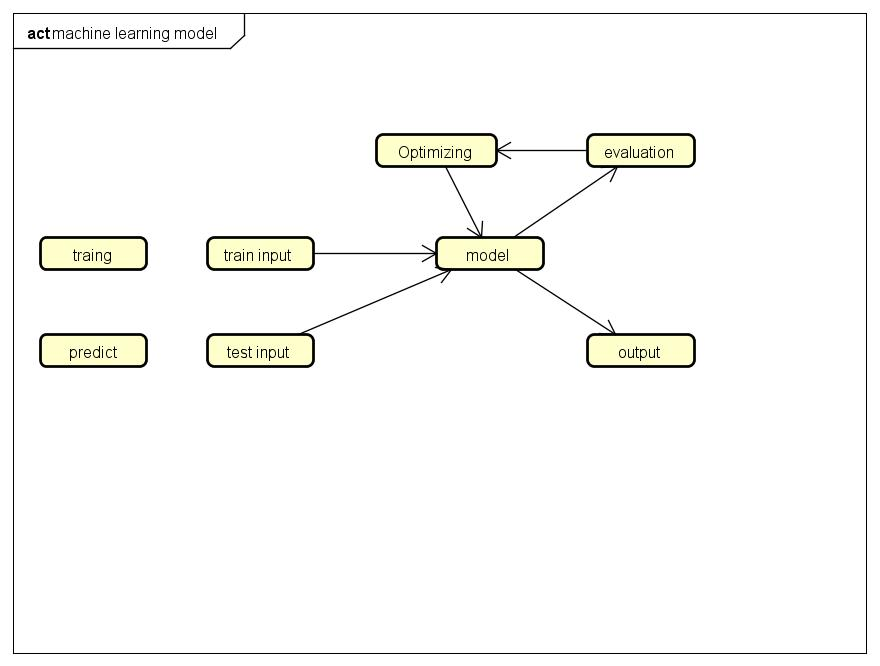
\includegraphics{ml__model.jpg}

\#\#

by Cloud.yu 2018-3-10

    \begin{figure}
\centering
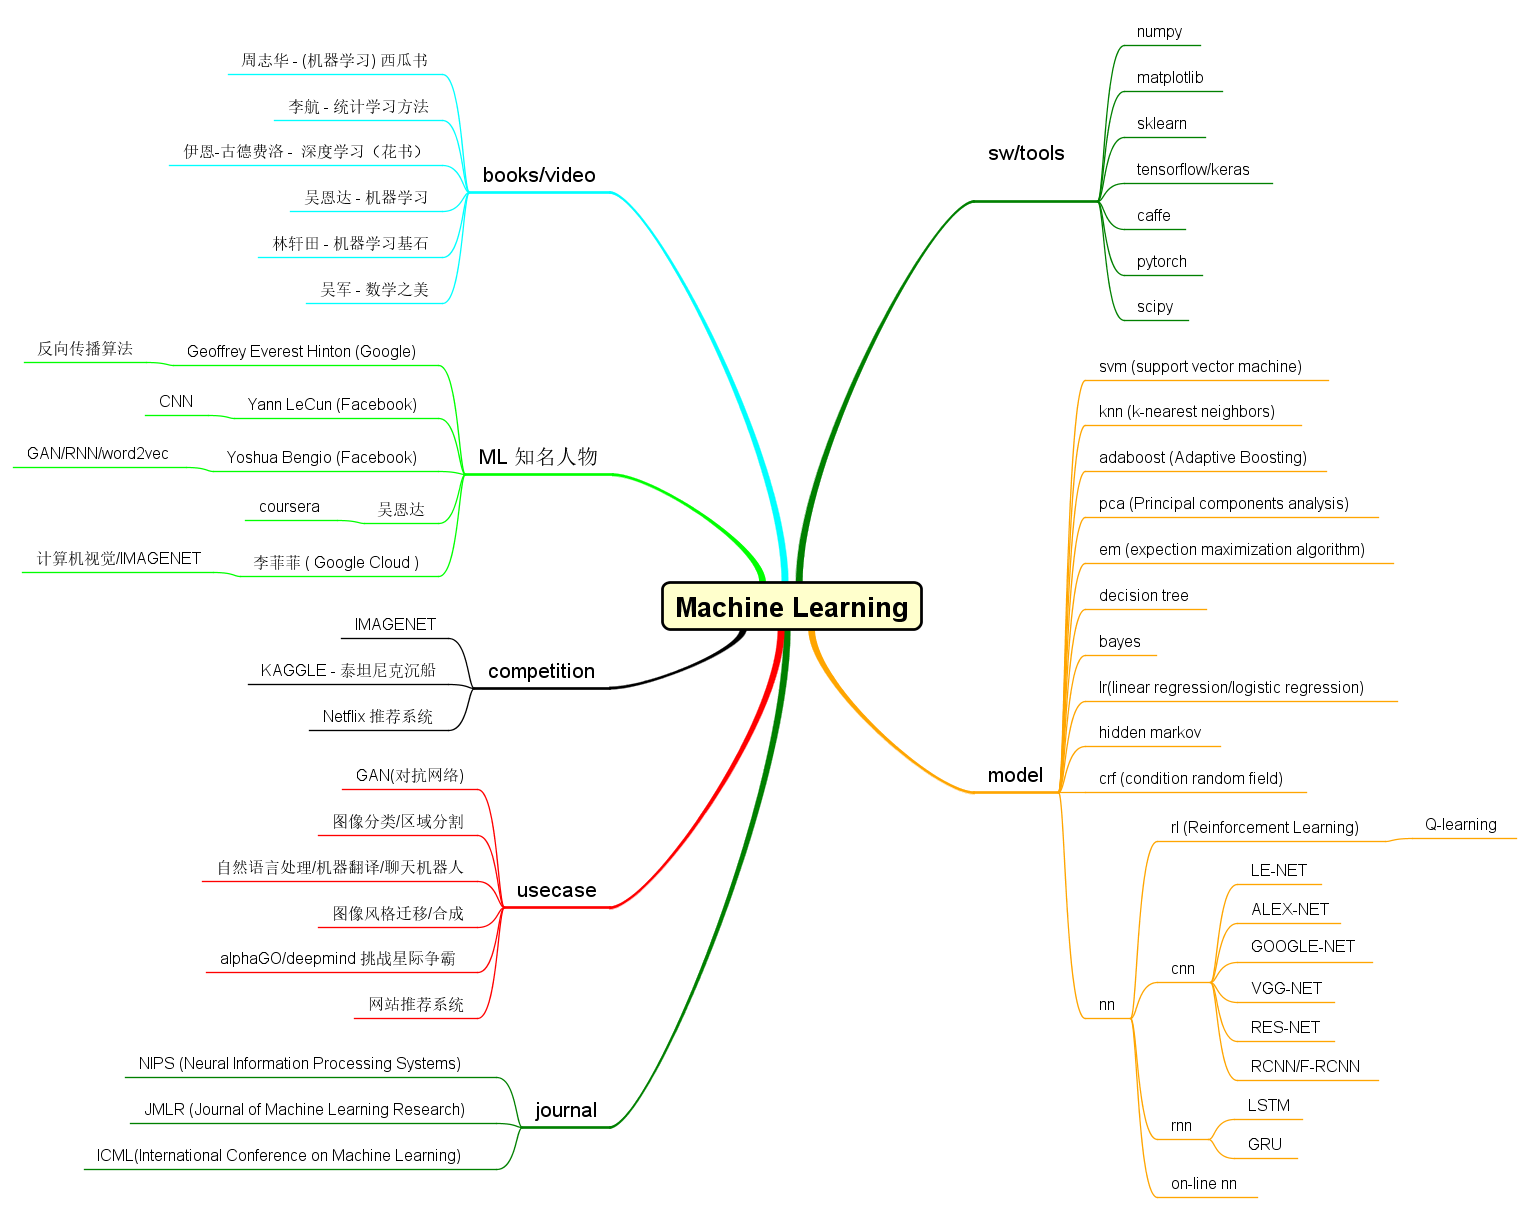
\includegraphics{mlmindmap.png}
\caption{}
\end{figure}

    \begin{figure}
\centering
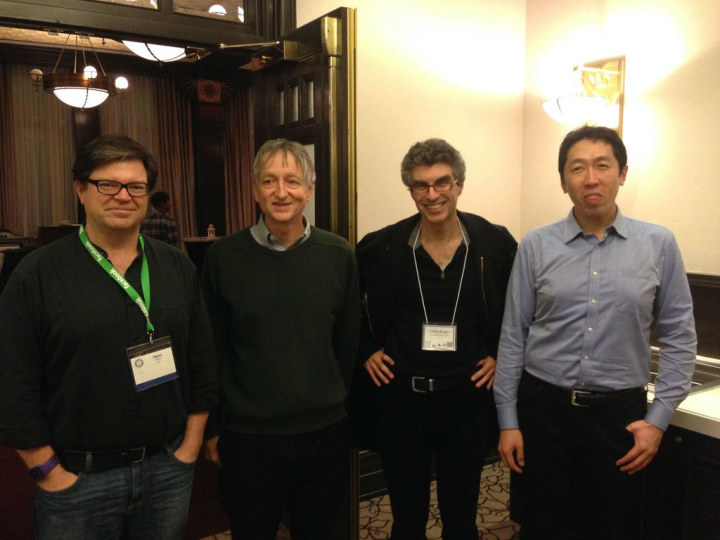
\includegraphics{ml_people.jpg}
\caption{}
\end{figure}

    \begin{figure}
\centering
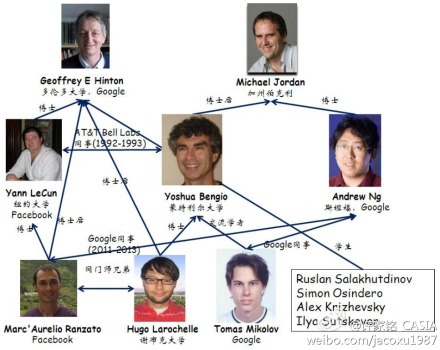
\includegraphics{ml_relation.jpg}
\caption{}
\end{figure}

    \#

Perceptron (感知机)

\begin{center}\rule{0.5\linewidth}{\linethickness}\end{center}

\textbf{任务} : 求一条线\(wx+b=0\) 对不同类别的点进行二分类 ****
\textbf{类型} : 监督学习

\textbf{模型} : 感知机 \(f(x)=sign(wx+b)\), 其中\(w\)叫做权重(weight),
\(b\)叫做偏置(bias)

\textbf{评价方法} : \(\min \{ \sum {{\rm{(y(wx + b) < 0)}}} \}\)

\textbf{优化方法} : PLA/Pocket

    \begin{center}\rule{0.5\linewidth}{\linethickness}\end{center}

\#

PLA (Percetron Learning Algorithm)

\begin{longtable}[]{@{}l@{}}
\toprule
- \textbf{Input}: traing data
(\(T = \{(x_{0}, y_{0}), (x_{1}, y_{1}), ..., (x_{i}, y_{i})\}\))\tabularnewline
- \textbf{Output}: \((w, b)\)\tabularnewline
- init \((w, b)\rightarrow(0,0)\) , \(i\rightarrow 0\)\tabularnewline
- while \(i != len(T)\) do\tabularnewline
- if \(y_{i}(wx_{i}+b) <= 0\) then\tabularnewline
- \((w, b) \rightarrow (w, b) + y_{i}x_{i}\)\tabularnewline
- \(i\rightarrow 0\)\tabularnewline
- else\tabularnewline
- \(i=i+1\)\tabularnewline
- end if\tabularnewline
- end while\tabularnewline
\bottomrule
\end{longtable}

    \begin{figure}
\centering
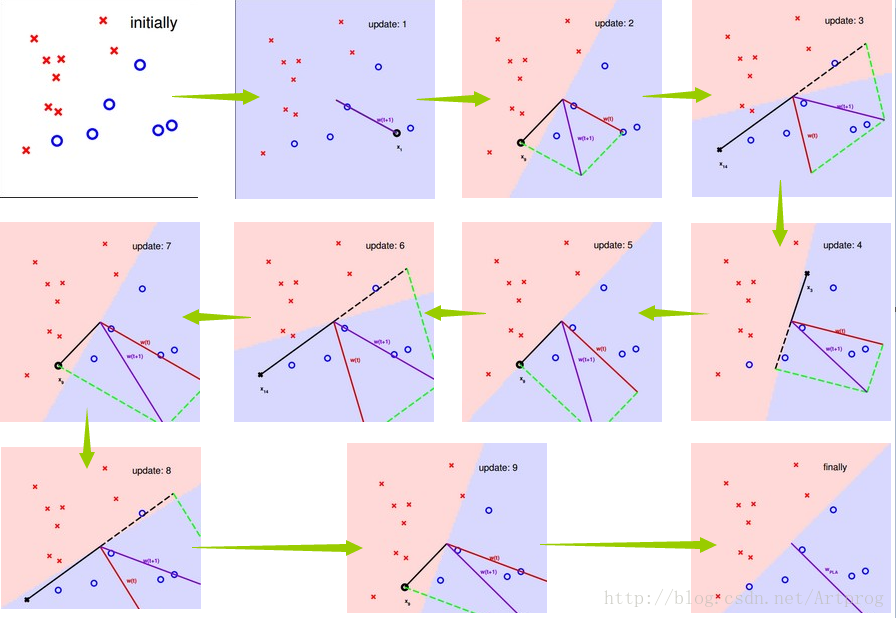
\includegraphics{pla.png}
\caption{}
\end{figure}

    \begin{Verbatim}[commandchars=\\\{\}]
{\color{incolor}In [{\color{incolor}3}]:} \PY{k+kn}{import} \PY{n+nn}{numpy} \PY{k}{as} \PY{n+nn}{np}
        \PY{k+kn}{import} \PY{n+nn}{matplotlib}
        \PY{k+kn}{import} \PY{n+nn}{matplotlib}\PY{n+nn}{.}\PY{n+nn}{pyplot} \PY{k}{as} \PY{n+nn}{plt} 
        
        \PY{n}{LEN} \PY{o}{=} \PY{l+m+mi}{40}
        \PY{n}{x} \PY{o}{=} \PY{n}{np}\PY{o}{.}\PY{n}{random}\PY{o}{.}\PY{n}{randint}\PY{p}{(}\PY{o}{\PYZhy{}}\PY{l+m+mi}{5}\PY{p}{,}\PY{l+m+mi}{5}\PY{p}{,} \PY{p}{(}\PY{n}{LEN}\PY{p}{,}\PY{l+m+mi}{2}\PY{p}{)}\PY{p}{)}
        \PY{n}{line} \PY{o}{=} \PY{n}{np}\PY{o}{.}\PY{n}{random}\PY{o}{.}\PY{n}{randint}\PY{p}{(}\PY{o}{\PYZhy{}}\PY{l+m+mi}{5}\PY{p}{,}\PY{l+m+mi}{5}\PY{p}{,} \PY{p}{(}\PY{l+m+mi}{2}\PY{p}{,} \PY{l+m+mi}{1}\PY{p}{)}\PY{p}{)}
        \PY{c+c1}{\PYZsh{}  2y \PYZhy{} 3x}
        \PY{n}{label} \PY{o}{=} \PY{n}{np}\PY{o}{.}\PY{n}{sign}\PY{p}{(}\PY{n}{np}\PY{o}{.}\PY{n}{dot}\PY{p}{(}\PY{n}{x}\PY{p}{,} \PY{n}{line}\PY{p}{)}\PY{p}{)}
        \PY{n}{label}\PY{p}{[}\PY{n}{label} \PY{o}{==} \PY{l+m+mi}{0}\PY{p}{]} \PY{o}{=} \PY{l+m+mi}{1}
        \PY{n}{fig} \PY{o}{=} \PY{n}{plt}\PY{o}{.}\PY{n}{figure}\PY{p}{(}\PY{l+m+mi}{1}\PY{p}{)}
        \PY{n}{idx\PYZus{}0} \PY{o}{=} \PY{n}{np}\PY{o}{.}\PY{n}{where}\PY{p}{(}\PY{n}{label}\PY{p}{[}\PY{p}{:}\PY{p}{,} \PY{l+m+mi}{0}\PY{p}{]} \PY{o}{==} \PY{o}{\PYZhy{}}\PY{l+m+mi}{1}\PY{p}{)}
        \PY{n}{p0} \PY{o}{=} \PY{n}{plt}\PY{o}{.}\PY{n}{scatter}\PY{p}{(}\PY{n}{x}\PY{p}{[}\PY{n}{idx\PYZus{}0}\PY{p}{,}\PY{l+m+mi}{1}\PY{p}{]}\PY{p}{,} \PY{n}{x}\PY{p}{[}\PY{n}{idx\PYZus{}0}\PY{p}{,}\PY{l+m+mi}{0}\PY{p}{]}\PY{p}{,} \PY{n}{marker} \PY{o}{=} \PY{l+s+s1}{\PYZsq{}}\PY{l+s+s1}{+}\PY{l+s+s1}{\PYZsq{}}\PY{p}{,} \PY{n}{color} \PY{o}{=} \PY{l+s+s1}{\PYZsq{}}\PY{l+s+s1}{c}\PY{l+s+s1}{\PYZsq{}}\PY{p}{,} \PY{n}{label}\PY{o}{=}\PY{l+s+s1}{\PYZsq{}}\PY{l+s+s1}{\PYZhy{}1}\PY{l+s+s1}{\PYZsq{}}\PY{p}{,} \PY{n}{s} \PY{o}{=} \PY{l+m+mi}{50}\PY{p}{)}
        \PY{n}{idx\PYZus{}1} \PY{o}{=} \PY{n}{np}\PY{o}{.}\PY{n}{where}\PY{p}{(}\PY{n}{label}\PY{p}{[}\PY{p}{:}\PY{p}{,} \PY{l+m+mi}{0}\PY{p}{]} \PY{o}{==} \PY{l+m+mi}{1}\PY{p}{)}
        \PY{n}{p1} \PY{o}{=} \PY{n}{plt}\PY{o}{.}\PY{n}{scatter}\PY{p}{(}\PY{n}{x}\PY{p}{[}\PY{n}{idx\PYZus{}1}\PY{p}{,}\PY{l+m+mi}{1}\PY{p}{]}\PY{p}{,} \PY{n}{x}\PY{p}{[}\PY{n}{idx\PYZus{}1}\PY{p}{,}\PY{l+m+mi}{0}\PY{p}{]}\PY{p}{,} \PY{n}{marker} \PY{o}{=} \PY{l+s+s1}{\PYZsq{}}\PY{l+s+s1}{x}\PY{l+s+s1}{\PYZsq{}}\PY{p}{,} \PY{n}{color} \PY{o}{=} \PY{l+s+s1}{\PYZsq{}}\PY{l+s+s1}{m}\PY{l+s+s1}{\PYZsq{}}\PY{p}{,} \PY{n}{label}\PY{o}{=}\PY{l+s+s1}{\PYZsq{}}\PY{l+s+s1}{1}\PY{l+s+s1}{\PYZsq{}}\PY{p}{,} \PY{n}{s} \PY{o}{=} \PY{l+m+mi}{50}\PY{p}{)}
        \PY{n}{plt}\PY{o}{.}\PY{n}{title}\PY{p}{(}\PY{l+s+s1}{\PYZsq{}}\PY{l+s+s1}{PLA}\PY{l+s+s1}{\PYZsq{}}\PY{p}{)}
        \PY{n}{plt}\PY{o}{.}\PY{n}{xlabel}\PY{p}{(}\PY{l+s+s1}{\PYZsq{}}\PY{l+s+s1}{x}\PY{l+s+s1}{\PYZsq{}}\PY{p}{)}
        \PY{n}{plt}\PY{o}{.}\PY{n}{ylabel}\PY{p}{(}\PY{l+s+s1}{\PYZsq{}}\PY{l+s+s1}{y}\PY{l+s+s1}{\PYZsq{}}\PY{p}{)}
        \PY{n}{plt}\PY{o}{.}\PY{n}{xlim}\PY{p}{(}\PY{p}{(}\PY{o}{\PYZhy{}}\PY{l+m+mi}{6}\PY{p}{,}\PY{l+m+mi}{6}\PY{p}{)}\PY{p}{)}
        \PY{n}{plt}\PY{o}{.}\PY{n}{ylim}\PY{p}{(}\PY{p}{(}\PY{o}{\PYZhy{}}\PY{l+m+mi}{6}\PY{p}{,}\PY{l+m+mi}{6}\PY{p}{)}\PY{p}{)}
        \PY{n}{plt}\PY{o}{.}\PY{n}{legend}\PY{p}{(}\PY{p}{)}
        \PY{n}{plt}\PY{o}{.}\PY{n}{grid}\PY{p}{(}\PY{k+kc}{True}\PY{p}{)}
        \PY{n}{plt}\PY{o}{.}\PY{n}{show}\PY{p}{(}\PY{p}{)}
\end{Verbatim}


    \begin{center}
    \adjustimage{max size={0.9\linewidth}{0.9\paperheight}}{ml_files/ml_7_0.png}
    \end{center}
    { \hspace*{\fill} \\}
    
    \begin{Verbatim}[commandchars=\\\{\}]
{\color{incolor}In [{\color{incolor}4}]:} \PY{n}{cnt} \PY{o}{=} \PY{l+m+mi}{0}
        \PY{n}{pla} \PY{o}{=} \PY{n}{np}\PY{o}{.}\PY{n}{zeros}\PY{p}{(}\PY{p}{(}\PY{l+m+mi}{2}\PY{p}{,}\PY{l+m+mi}{1}\PY{p}{)}\PY{p}{)}
        \PY{n}{\PYZus{}update} \PY{o}{=} \PY{l+m+mi}{0}
        
        \PY{k}{while} \PY{n}{cnt}\PY{o}{\PYZlt{}}\PY{n}{LEN}\PY{p}{:}
            \PY{n}{\PYZus{}update} \PY{o}{=} \PY{n}{np}\PY{o}{.}\PY{n}{sign}\PY{p}{(}\PY{n}{np}\PY{o}{.}\PY{n}{dot}\PY{p}{(}\PY{n}{x}\PY{p}{[}\PY{n}{cnt}\PY{p}{,}\PY{p}{:}\PY{p}{]}\PY{p}{,} \PY{n}{pla}\PY{p}{)}\PY{p}{)} \PY{o}{*} \PY{n}{label}\PY{p}{[}\PY{n}{cnt}\PY{p}{,} \PY{l+m+mi}{0}\PY{p}{]}
            \PY{k}{if} \PY{n}{\PYZus{}update} \PY{o}{\PYZlt{}}\PY{o}{=} \PY{l+m+mi}{0}\PY{p}{:}
                \PY{n}{\PYZus{}x} \PY{o}{=} \PY{n}{x}\PY{p}{[}\PY{n}{cnt}\PY{p}{,} \PY{p}{:}\PY{p}{]}
                \PY{n}{\PYZus{}x}\PY{o}{.}\PY{n}{shape} \PY{o}{=} \PY{p}{(}\PY{l+m+mi}{1}\PY{p}{,}\PY{l+m+mi}{2}\PY{p}{)}
                \PY{n}{\PYZus{}x} \PY{o}{=} \PY{n}{np}\PY{o}{.}\PY{n}{transpose}\PY{p}{(}\PY{n}{\PYZus{}x}\PY{p}{)}
                \PY{n}{pla} \PY{o}{=} \PY{n}{pla} \PY{o}{+} \PY{n}{\PYZus{}x}\PY{o}{*}\PY{n}{label}\PY{p}{[}\PY{n}{cnt}\PY{p}{,} \PY{l+m+mi}{0}\PY{p}{]}
                \PY{n}{cnt} \PY{o}{=} \PY{l+m+mi}{0}
            \PY{k}{else}\PY{p}{:}
                \PY{n}{cnt} \PY{o}{=} \PY{n}{cnt}\PY{o}{+}\PY{l+m+mi}{1}
                \PY{k}{continue}
        \PY{n+nb}{print}\PY{p}{(}\PY{n}{pla}\PY{p}{)}
        
        
        
            
\end{Verbatim}


    \begin{Verbatim}[commandchars=\\\{\}]
[[-3.]
 [-7.]]

    \end{Verbatim}

    \begin{Verbatim}[commandchars=\\\{\}]
{\color{incolor}In [{\color{incolor}5}]:} \PY{n}{fig} \PY{o}{=} \PY{n}{plt}\PY{o}{.}\PY{n}{figure}\PY{p}{(}\PY{l+m+mi}{1}\PY{p}{)}
        \PY{n}{idx\PYZus{}0} \PY{o}{=} \PY{n}{np}\PY{o}{.}\PY{n}{where}\PY{p}{(}\PY{n}{label}\PY{p}{[}\PY{p}{:}\PY{p}{,} \PY{l+m+mi}{0}\PY{p}{]} \PY{o}{==} \PY{o}{\PYZhy{}}\PY{l+m+mi}{1}\PY{p}{)}
        \PY{n}{p0} \PY{o}{=} \PY{n}{plt}\PY{o}{.}\PY{n}{scatter}\PY{p}{(}\PY{n}{x}\PY{p}{[}\PY{n}{idx\PYZus{}0}\PY{p}{,}\PY{l+m+mi}{1}\PY{p}{]}\PY{p}{,} \PY{n}{x}\PY{p}{[}\PY{n}{idx\PYZus{}0}\PY{p}{,}\PY{l+m+mi}{0}\PY{p}{]}\PY{p}{,} \PY{n}{marker} \PY{o}{=} \PY{l+s+s1}{\PYZsq{}}\PY{l+s+s1}{+}\PY{l+s+s1}{\PYZsq{}}\PY{p}{,} \PY{n}{color} \PY{o}{=} \PY{l+s+s1}{\PYZsq{}}\PY{l+s+s1}{c}\PY{l+s+s1}{\PYZsq{}}\PY{p}{,} \PY{n}{label}\PY{o}{=}\PY{l+s+s1}{\PYZsq{}}\PY{l+s+s1}{\PYZhy{}1}\PY{l+s+s1}{\PYZsq{}}\PY{p}{,} \PY{n}{s} \PY{o}{=} \PY{l+m+mi}{50}\PY{p}{)}
        \PY{n}{idx\PYZus{}1} \PY{o}{=} \PY{n}{np}\PY{o}{.}\PY{n}{where}\PY{p}{(}\PY{n}{label}\PY{p}{[}\PY{p}{:}\PY{p}{,} \PY{l+m+mi}{0}\PY{p}{]} \PY{o}{==} \PY{l+m+mi}{1}\PY{p}{)}
        \PY{n}{p1} \PY{o}{=} \PY{n}{plt}\PY{o}{.}\PY{n}{scatter}\PY{p}{(}\PY{n}{x}\PY{p}{[}\PY{n}{idx\PYZus{}1}\PY{p}{,}\PY{l+m+mi}{1}\PY{p}{]}\PY{p}{,} \PY{n}{x}\PY{p}{[}\PY{n}{idx\PYZus{}1}\PY{p}{,}\PY{l+m+mi}{0}\PY{p}{]}\PY{p}{,} \PY{n}{marker} \PY{o}{=} \PY{l+s+s1}{\PYZsq{}}\PY{l+s+s1}{x}\PY{l+s+s1}{\PYZsq{}}\PY{p}{,} \PY{n}{color} \PY{o}{=} \PY{l+s+s1}{\PYZsq{}}\PY{l+s+s1}{m}\PY{l+s+s1}{\PYZsq{}}\PY{p}{,} \PY{n}{label}\PY{o}{=}\PY{l+s+s1}{\PYZsq{}}\PY{l+s+s1}{1}\PY{l+s+s1}{\PYZsq{}}\PY{p}{,} \PY{n}{s} \PY{o}{=} \PY{l+m+mi}{50}\PY{p}{)}
        \PY{n}{plt}\PY{o}{.}\PY{n}{title}\PY{p}{(}\PY{l+s+s1}{\PYZsq{}}\PY{l+s+s1}{PLA}\PY{l+s+s1}{\PYZsq{}}\PY{p}{)}
        \PY{n}{plt}\PY{o}{.}\PY{n}{xlabel}\PY{p}{(}\PY{l+s+s1}{\PYZsq{}}\PY{l+s+s1}{x}\PY{l+s+s1}{\PYZsq{}}\PY{p}{)}
        \PY{n}{plt}\PY{o}{.}\PY{n}{ylabel}\PY{p}{(}\PY{l+s+s1}{\PYZsq{}}\PY{l+s+s1}{y}\PY{l+s+s1}{\PYZsq{}}\PY{p}{)}
        \PY{n}{plt}\PY{o}{.}\PY{n}{xlim}\PY{p}{(}\PY{p}{(}\PY{o}{\PYZhy{}}\PY{l+m+mi}{6}\PY{p}{,}\PY{l+m+mi}{6}\PY{p}{)}\PY{p}{)}
        \PY{n}{plt}\PY{o}{.}\PY{n}{ylim}\PY{p}{(}\PY{p}{(}\PY{o}{\PYZhy{}}\PY{l+m+mi}{6}\PY{p}{,}\PY{l+m+mi}{6}\PY{p}{)}\PY{p}{)}
        \PY{n}{plt}\PY{o}{.}\PY{n}{legend}\PY{p}{(}\PY{p}{)}
        \PY{n}{plt}\PY{o}{.}\PY{n}{grid}\PY{p}{(}\PY{k+kc}{True}\PY{p}{)}
        
        \PY{n}{k} \PY{o}{=} \PY{o}{\PYZhy{}}\PY{n}{pla}\PY{p}{[}\PY{l+m+mi}{1}\PY{p}{,}\PY{p}{:}\PY{p}{]} \PY{o}{/} \PY{n}{pla}\PY{p}{[}\PY{l+m+mi}{0}\PY{p}{,}\PY{p}{:}\PY{p}{]}
        \PY{n}{line\PYZus{}x} \PY{o}{=} \PY{n}{np}\PY{o}{.}\PY{n}{linspace}\PY{p}{(}\PY{o}{\PYZhy{}}\PY{l+m+mi}{5}\PY{p}{,}\PY{l+m+mi}{5}\PY{p}{,}\PY{l+m+mi}{50}\PY{p}{)} 
        \PY{n}{line\PYZus{}y} \PY{o}{=} \PY{n}{k}\PY{o}{*}\PY{n}{line\PYZus{}x}
        \PY{n}{plt}\PY{o}{.}\PY{n}{plot}\PY{p}{(}\PY{n}{line\PYZus{}x}\PY{p}{,}\PY{n}{line\PYZus{}y}\PY{p}{)}
        \PY{n}{plt}\PY{o}{.}\PY{n}{show}\PY{p}{(}\PY{p}{)}
\end{Verbatim}


    \begin{center}
    \adjustimage{max size={0.9\linewidth}{0.9\paperheight}}{ml_files/ml_9_0.png}
    \end{center}
    { \hspace*{\fill} \\}
    
    \begin{center}\rule{0.5\linewidth}{\linethickness}\end{center}

\#

POCKET Algorithm

\begin{longtable}[]{@{}l@{}}
\toprule
- \textbf{Input}: traing data
(\(T = \{(x_{0}, y_{0}), (x_{1}, y_{1}), ..., (x_{i}, y_{i})\}\))\tabularnewline
- \textbf{Output}: \((w, b)\)\tabularnewline
- init \((w_{best}, b_{best}) \rightarrow random\)\tabularnewline
-
\(loss_{min} \leftarrow sum(sign(w_{best}x + b_{best}) != y)\)\tabularnewline
- for \(i= 0\rightarrow1000\) do\tabularnewline
- init \((w, b)\rightarrow random\) and
\(j\rightarrow 0\)\tabularnewline
- Save error label data to
\(T_{error} = \{(x_{0}, y_{0}), (x_{1}, y_{1}), ..., (x_{err}, y_{err})\}\)\tabularnewline
- while \(j != len(T_{error})\) do\tabularnewline
- \((\bar{w}, \bar{b}) \rightarrow (w, b) + y_{j}x_{j}\)\tabularnewline
- \(loss \leftarrow sum(sign(\bar{w}x + \bar{b}) != y)\)\tabularnewline
- if \(loss < loss_{min}\) then\tabularnewline
- break\tabularnewline
- end if\tabularnewline
- \(j=j+1\)\tabularnewline
- end while\tabularnewline
- if \(j != len(y_{err})\)\tabularnewline
- \((w_{best}, b_{best}) \leftarrow (\bar{w}, \bar{b})\)\tabularnewline
- \(loss_{min} \leftarrow loss\)\tabularnewline
- end if\tabularnewline
- j = 0\tabularnewline
- end for\tabularnewline
\bottomrule
\end{longtable}

    \begin{Verbatim}[commandchars=\\\{\}]
{\color{incolor}In [{\color{incolor}6}]:} \PY{k}{def} \PY{n+nf}{cal\PYZus{}loss}\PY{p}{(}\PY{n}{\PYZus{}pocket}\PY{p}{,} \PY{n}{\PYZus{}x}\PY{p}{,} \PY{n}{\PYZus{}label}\PY{p}{)}\PY{p}{:}
            \PY{n}{\PYZus{}cal} \PY{o}{=} \PY{n}{np}\PY{o}{.}\PY{n}{sign}\PY{p}{(}\PY{n}{np}\PY{o}{.}\PY{n}{dot}\PY{p}{(}\PY{n}{\PYZus{}x}\PY{p}{,} \PY{n}{\PYZus{}pocket}\PY{p}{)}\PY{p}{)}
            \PY{n}{\PYZus{}cal}\PY{o}{.}\PY{n}{shape} \PY{o}{=} \PY{p}{(}\PY{l+m+mi}{40}\PY{p}{,}\PY{l+m+mi}{1}\PY{p}{)}
            \PY{n}{idx} \PY{o}{=} \PY{n}{np}\PY{o}{.}\PY{n}{where}\PY{p}{(}\PY{n}{\PYZus{}cal}\PY{p}{[}\PY{p}{:}\PY{p}{,} \PY{l+m+mi}{0}\PY{p}{]} \PY{o}{!=} \PY{n}{\PYZus{}label}\PY{p}{[}\PY{p}{:}\PY{p}{,} \PY{l+m+mi}{0}\PY{p}{]}\PY{p}{)}
            \PY{n}{loss} \PY{o}{=} \PY{n}{np}\PY{o}{.}\PY{n}{sum}\PY{p}{(}\PY{n}{\PYZus{}cal}\PY{p}{[}\PY{p}{:}\PY{p}{,} \PY{l+m+mi}{0}\PY{p}{]} \PY{o}{!=} \PY{n}{\PYZus{}label}\PY{p}{[}\PY{p}{:}\PY{p}{,} \PY{l+m+mi}{0}\PY{p}{]}\PY{p}{)}
            \PY{k}{return} \PY{n+nb}{list}\PY{p}{(}\PY{n}{idx}\PY{p}{[}\PY{l+m+mi}{0}\PY{p}{]}\PY{p}{)}\PY{p}{,} \PY{n}{loss}
        
        \PY{c+c1}{\PYZsh{} random init best pocket and min loss value}
        \PY{n}{pocket\PYZus{}best} \PY{o}{=} \PY{n}{np}\PY{o}{.}\PY{n}{random}\PY{o}{.}\PY{n}{randint}\PY{p}{(}\PY{o}{\PYZhy{}}\PY{l+m+mi}{5}\PY{p}{,}\PY{l+m+mi}{5}\PY{p}{,} \PY{p}{(}\PY{l+m+mi}{2}\PY{p}{,}\PY{l+m+mi}{1}\PY{p}{)}\PY{p}{)}
        \PY{n}{\PYZus{}}\PY{p}{,} \PY{n}{min\PYZus{}loss} \PY{o}{=} \PY{n}{cal\PYZus{}loss}\PY{p}{(}\PY{n}{pocket\PYZus{}best}\PY{p}{,} \PY{n}{x}\PY{p}{,} \PY{n}{label}\PY{p}{)}
        
        
        \PY{k}{for} \PY{n}{i} \PY{o+ow}{in} \PY{n+nb}{range}\PY{p}{(}\PY{l+m+mi}{15}\PY{p}{)}\PY{p}{:}
            \PY{c+c1}{\PYZsh{} random pocket and cur loss for each period}
            \PY{n}{pocket} \PY{o}{=} \PY{n}{np}\PY{o}{.}\PY{n}{random}\PY{o}{.}\PY{n}{randint}\PY{p}{(}\PY{o}{\PYZhy{}}\PY{l+m+mi}{5}\PY{p}{,}\PY{l+m+mi}{5}\PY{p}{,} \PY{p}{(}\PY{l+m+mi}{2}\PY{p}{,}\PY{l+m+mi}{1}\PY{p}{)}\PY{p}{)}
            \PY{n}{\PYZus{}pocket} \PY{o}{=} \PY{n}{pocket}
            \PY{n}{idx}\PY{p}{,} \PY{n}{cur\PYZus{}loss} \PY{o}{=} \PY{n}{cal\PYZus{}loss}\PY{p}{(}\PY{n}{pocket}\PY{p}{,} \PY{n}{x}\PY{p}{,} \PY{n}{label}\PY{p}{)}
            \PY{k}{while} \PY{n}{cnt} \PY{o}{\PYZlt{}} \PY{n+nb}{len}\PY{p}{(}\PY{n}{idx}\PY{p}{)}\PY{p}{:}
                \PY{n}{\PYZus{}x} \PY{o}{=} \PY{n}{x}\PY{p}{[}\PY{n}{idx}\PY{p}{[}\PY{n}{cnt}\PY{p}{]}\PY{p}{,} \PY{p}{:}\PY{p}{]}
                \PY{n}{\PYZus{}x}\PY{o}{.}\PY{n}{shape} \PY{o}{=} \PY{p}{(}\PY{l+m+mi}{2}\PY{p}{,}\PY{l+m+mi}{1}\PY{p}{)}
                \PY{n}{\PYZus{}pocket} \PY{o}{=} \PY{n}{pocket} \PY{o}{+} \PY{n}{\PYZus{}x} \PY{o}{*} \PY{n}{label}\PY{p}{[}\PY{n}{idx}\PY{p}{[}\PY{n}{cnt}\PY{p}{]}\PY{p}{,} \PY{l+m+mi}{0}\PY{p}{]}
                \PY{n}{\PYZus{}}\PY{p}{,} \PY{n}{cur\PYZus{}loss} \PY{o}{=} \PY{n}{cal\PYZus{}loss}\PY{p}{(}\PY{n}{\PYZus{}pocket}\PY{p}{,} \PY{n}{x}\PY{p}{,} \PY{n}{label}\PY{p}{)}
                \PY{c+c1}{\PYZsh{} compare cur loss with min loss}
                \PY{k}{if} \PY{n}{cur\PYZus{}loss} \PY{o}{\PYZlt{}} \PY{n}{min\PYZus{}loss}\PY{p}{:}
                    \PY{k}{break}
                \PY{k}{else}\PY{p}{:}
                    \PY{n}{cnt} \PY{o}{=} \PY{n}{cnt} \PY{o}{+} \PY{l+m+mi}{1}
            \PY{k}{if} \PY{n}{cnt} \PY{o}{!=} \PY{n+nb}{len}\PY{p}{(}\PY{n}{idx}\PY{p}{)}\PY{p}{:}
                \PY{n}{pocket\PYZus{}best} \PY{o}{=} \PY{n}{\PYZus{}pocket}
                \PY{n}{\PYZus{}}\PY{p}{,} \PY{n}{min\PYZus{}loss} \PY{o}{=} \PY{n}{cal\PYZus{}loss}\PY{p}{(}\PY{n}{pocket\PYZus{}best}\PY{p}{,} \PY{n}{x}\PY{p}{,} \PY{n}{label}\PY{p}{)}
            \PY{n}{cnt} \PY{o}{=} \PY{l+m+mi}{0}
        
        \PY{n}{pocket} \PY{o}{=} \PY{n}{pocket\PYZus{}best}
        \PY{n+nb}{print}\PY{p}{(}\PY{n}{pocket}\PY{p}{)}
\end{Verbatim}


    \begin{Verbatim}[commandchars=\\\{\}]
[[-2]
 [-4]]

    \end{Verbatim}

    \begin{Verbatim}[commandchars=\\\{\}]
{\color{incolor}In [{\color{incolor}7}]:} \PY{n}{fig} \PY{o}{=} \PY{n}{plt}\PY{o}{.}\PY{n}{figure}\PY{p}{(}\PY{l+m+mi}{1}\PY{p}{)}
        \PY{n}{idx\PYZus{}0} \PY{o}{=} \PY{n}{np}\PY{o}{.}\PY{n}{where}\PY{p}{(}\PY{n}{label}\PY{p}{[}\PY{p}{:}\PY{p}{,} \PY{l+m+mi}{0}\PY{p}{]} \PY{o}{==} \PY{o}{\PYZhy{}}\PY{l+m+mi}{1}\PY{p}{)}
        \PY{n}{p0} \PY{o}{=} \PY{n}{plt}\PY{o}{.}\PY{n}{scatter}\PY{p}{(}\PY{n}{x}\PY{p}{[}\PY{n}{idx\PYZus{}0}\PY{p}{,}\PY{l+m+mi}{1}\PY{p}{]}\PY{p}{,} \PY{n}{x}\PY{p}{[}\PY{n}{idx\PYZus{}0}\PY{p}{,}\PY{l+m+mi}{0}\PY{p}{]}\PY{p}{,} \PY{n}{marker} \PY{o}{=} \PY{l+s+s1}{\PYZsq{}}\PY{l+s+s1}{+}\PY{l+s+s1}{\PYZsq{}}\PY{p}{,} \PY{n}{color} \PY{o}{=} \PY{l+s+s1}{\PYZsq{}}\PY{l+s+s1}{c}\PY{l+s+s1}{\PYZsq{}}\PY{p}{,} \PY{n}{label}\PY{o}{=}\PY{l+s+s1}{\PYZsq{}}\PY{l+s+s1}{\PYZhy{}1}\PY{l+s+s1}{\PYZsq{}}\PY{p}{,} \PY{n}{s} \PY{o}{=} \PY{l+m+mi}{50}\PY{p}{)}
        \PY{n}{idx\PYZus{}1} \PY{o}{=} \PY{n}{np}\PY{o}{.}\PY{n}{where}\PY{p}{(}\PY{n}{label}\PY{p}{[}\PY{p}{:}\PY{p}{,} \PY{l+m+mi}{0}\PY{p}{]} \PY{o}{==} \PY{l+m+mi}{1}\PY{p}{)}
        \PY{n}{p1} \PY{o}{=} \PY{n}{plt}\PY{o}{.}\PY{n}{scatter}\PY{p}{(}\PY{n}{x}\PY{p}{[}\PY{n}{idx\PYZus{}1}\PY{p}{,}\PY{l+m+mi}{1}\PY{p}{]}\PY{p}{,} \PY{n}{x}\PY{p}{[}\PY{n}{idx\PYZus{}1}\PY{p}{,}\PY{l+m+mi}{0}\PY{p}{]}\PY{p}{,} \PY{n}{marker} \PY{o}{=} \PY{l+s+s1}{\PYZsq{}}\PY{l+s+s1}{x}\PY{l+s+s1}{\PYZsq{}}\PY{p}{,} \PY{n}{color} \PY{o}{=} \PY{l+s+s1}{\PYZsq{}}\PY{l+s+s1}{m}\PY{l+s+s1}{\PYZsq{}}\PY{p}{,} \PY{n}{label}\PY{o}{=}\PY{l+s+s1}{\PYZsq{}}\PY{l+s+s1}{1}\PY{l+s+s1}{\PYZsq{}}\PY{p}{,} \PY{n}{s} \PY{o}{=} \PY{l+m+mi}{50}\PY{p}{)}
        \PY{n}{plt}\PY{o}{.}\PY{n}{title}\PY{p}{(}\PY{l+s+s1}{\PYZsq{}}\PY{l+s+s1}{POCKET}\PY{l+s+s1}{\PYZsq{}}\PY{p}{)}
        \PY{n}{plt}\PY{o}{.}\PY{n}{xlabel}\PY{p}{(}\PY{l+s+s1}{\PYZsq{}}\PY{l+s+s1}{x}\PY{l+s+s1}{\PYZsq{}}\PY{p}{)}
        \PY{n}{plt}\PY{o}{.}\PY{n}{ylabel}\PY{p}{(}\PY{l+s+s1}{\PYZsq{}}\PY{l+s+s1}{y}\PY{l+s+s1}{\PYZsq{}}\PY{p}{)}
        \PY{n}{plt}\PY{o}{.}\PY{n}{xlim}\PY{p}{(}\PY{p}{(}\PY{o}{\PYZhy{}}\PY{l+m+mi}{6}\PY{p}{,}\PY{l+m+mi}{6}\PY{p}{)}\PY{p}{)}
        \PY{n}{plt}\PY{o}{.}\PY{n}{ylim}\PY{p}{(}\PY{p}{(}\PY{o}{\PYZhy{}}\PY{l+m+mi}{6}\PY{p}{,}\PY{l+m+mi}{6}\PY{p}{)}\PY{p}{)}
        \PY{n}{plt}\PY{o}{.}\PY{n}{legend}\PY{p}{(}\PY{p}{)}
        \PY{n}{plt}\PY{o}{.}\PY{n}{grid}\PY{p}{(}\PY{k+kc}{True}\PY{p}{)}
        
        \PY{n}{k} \PY{o}{=} \PY{o}{\PYZhy{}}\PY{n}{pocket}\PY{p}{[}\PY{l+m+mi}{1}\PY{p}{,}\PY{p}{:}\PY{p}{]} \PY{o}{/} \PY{n}{pocket}\PY{p}{[}\PY{l+m+mi}{0}\PY{p}{,}\PY{p}{:}\PY{p}{]}
        \PY{n}{line\PYZus{}x} \PY{o}{=} \PY{n}{np}\PY{o}{.}\PY{n}{linspace}\PY{p}{(}\PY{o}{\PYZhy{}}\PY{l+m+mi}{5}\PY{p}{,}\PY{l+m+mi}{5}\PY{p}{,}\PY{l+m+mi}{50}\PY{p}{)} 
        \PY{n}{line\PYZus{}y} \PY{o}{=} \PY{n}{k}\PY{o}{*}\PY{n}{line\PYZus{}x}
        \PY{n}{plt}\PY{o}{.}\PY{n}{plot}\PY{p}{(}\PY{n}{line\PYZus{}x}\PY{p}{,}\PY{n}{line\PYZus{}y}\PY{p}{)}
        \PY{n}{plt}\PY{o}{.}\PY{n}{show}\PY{p}{(}\PY{p}{)}
\end{Verbatim}


    \begin{center}
    \adjustimage{max size={0.9\linewidth}{0.9\paperheight}}{ml_files/ml_12_0.png}
    \end{center}
    { \hspace*{\fill} \\}
    
    \begin{figure}
\centering
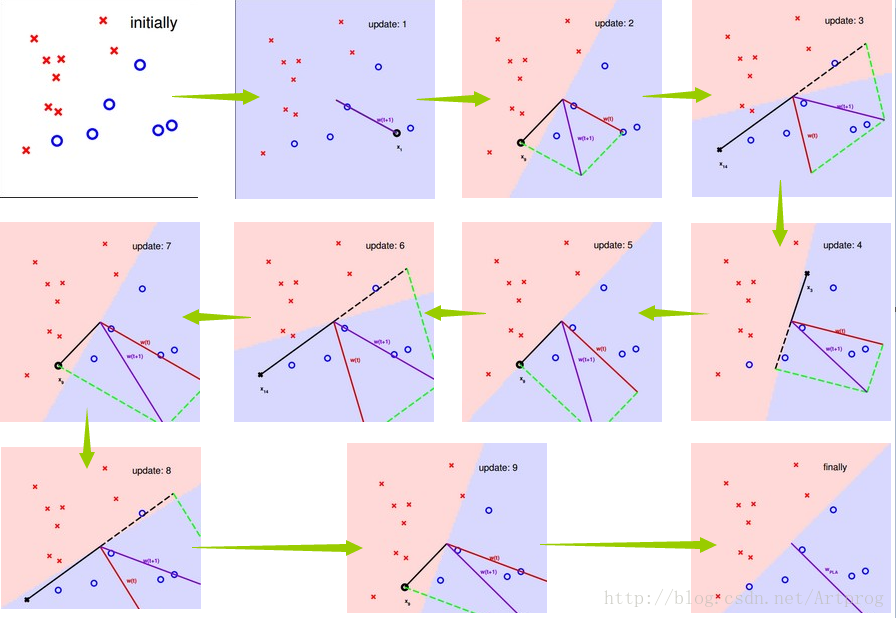
\includegraphics{assignment/perception/pla.gif}
\caption{}
\end{figure}

    \begin{figure}
\centering
\includegraphics{assignment/perception/pla_err.gif}
\caption{}
\end{figure}

    \begin{figure}
\centering
\includegraphics{assignment/perception/pocket.gif}
\caption{}
\end{figure}

    \#

SVM (Support Vector Machine)

\begin{center}\rule{0.5\linewidth}{\linethickness}\end{center}

\textbf{任务} : 对线性/非线性可分不同类别的点进行二分类 ****
\textbf{类型} : 监督学习

\textbf{模型} : \(f(x)=sign(wx+b)\)

\textbf{评价方法} :
\(\mathop {\min }\limits_{w,b} (\frac{1}{2}||w|{|^2}) + C\sum\limits_{i = 1}^m {\max (0,1 - {y_i}({w^T}{x_i}{\rm{ + }}b))}\)\\
\textgreater{}\emph{s.t.}
\({y_i}(w{x_{_i}} + b) - 1 \ge 0,i = 1,2,...,N\)

\textbf{优化方法} : 核技巧/SMO 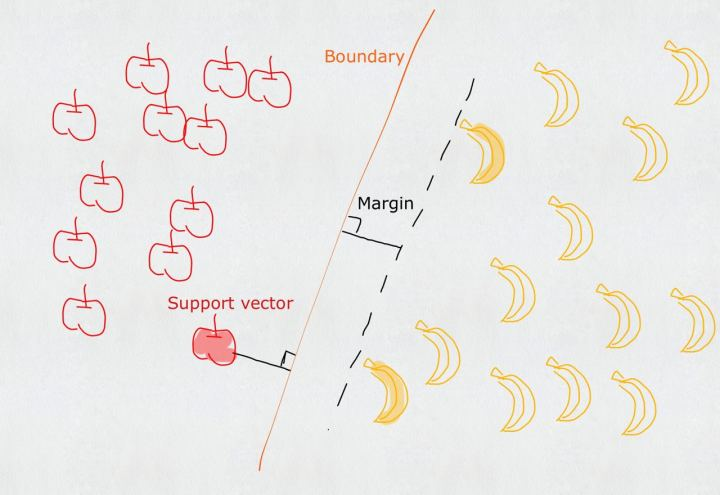
\includegraphics{svm.jpg}

    \#

核技巧

\textbf{核函数是二元函数,输入是变换之前的两个向量,其输出与两个向量变换之后的内积相等.
\(k({x_1},{x_2}) = f(x_1^T{x_2})\) } **** - 定义直线
\(y(x) = {w^T}x + b\) -
任意点\({x_0}\)到直线的距离为\(\frac{1}{{||w||}}({w^T}{x_0} + b)\) -
求在误分类最少的情况下的最大间距: \$\arg \mathop {\max }\limits\_\{w,b\}
\{ \frac{1}{{||w||}}\mathop {\min }\limits\_n
{[}\{y\_i\}(\{w\^{}T\}\{x\_i\} + b){]}\} \$ -
最大间距对偶形式:\(\arg \mathop {\max }\limits_\alpha \sum\limits_{i = 1}^N {{\alpha _i} - \frac{1}{2}\sum\limits_{i = 1}^N {\sum\limits_{j = 1}^N {{y_i}{y_j}} } } {\alpha _i}{\alpha _j}\langle {x_i},{x_{_j}}\rangle\)
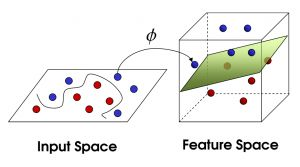
\includegraphics{svm_kernel.jpg} 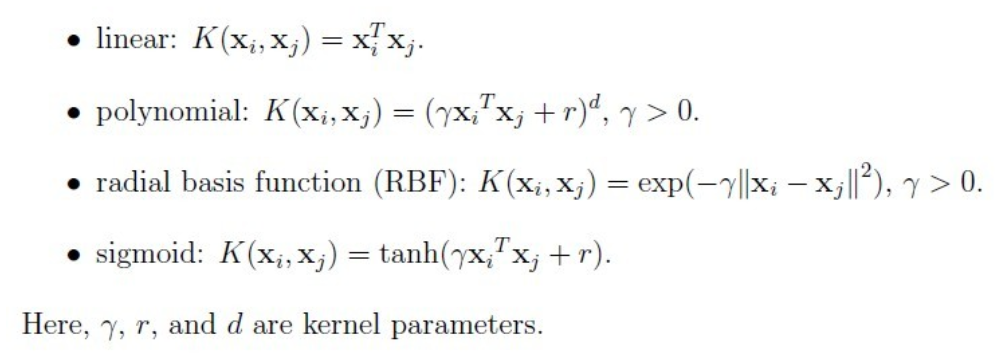
\includegraphics{核函数.png}

    \begin{Verbatim}[commandchars=\\\{\}]
{\color{incolor}In [{\color{incolor}5}]:} \PY{k+kn}{import} \PY{n+nn}{numpy} \PY{k}{as} \PY{n+nn}{np}
        \PY{k+kn}{import} \PY{n+nn}{matplotlib}\PY{n+nn}{.}\PY{n+nn}{pyplot} \PY{k}{as} \PY{n+nn}{plt}
        \PY{k+kn}{import} \PY{n+nn}{matplotlib}\PY{n+nn}{.}\PY{n+nn}{patches} \PY{k}{as} \PY{n+nn}{mpatches}
        \PY{k+kn}{from} \PY{n+nn}{matplotlib} \PY{k}{import} \PY{n}{style}
        \PY{n}{style}\PY{o}{.}\PY{n}{use}\PY{p}{(}\PY{l+s+s2}{\PYZdq{}}\PY{l+s+s2}{ggplot}\PY{l+s+s2}{\PYZdq{}}\PY{p}{)}
        \PY{k+kn}{from} \PY{n+nn}{sklearn} \PY{k}{import} \PY{n}{svm}
        \PY{k+kn}{from} \PY{n+nn}{sklearn}\PY{n+nn}{.}\PY{n+nn}{datasets}\PY{n+nn}{.}\PY{n+nn}{samples\PYZus{}generator} \PY{k}{import} \PY{n}{make\PYZus{}blobs}
        
        \PY{c+c1}{\PYZsh{}\PYZsh{} 测试数据生成}
        \PY{n}{\PYZus{}x} \PY{o}{=} \PY{n}{np}\PY{o}{.}\PY{n}{random}\PY{o}{.}\PY{n}{randint}\PY{p}{(}\PY{o}{\PYZhy{}}\PY{l+m+mi}{10}\PY{p}{,} \PY{l+m+mi}{10}\PY{p}{,} \PY{p}{(}\PY{l+m+mi}{400}\PY{p}{,} \PY{l+m+mi}{2}\PY{p}{)}\PY{p}{)}
        \PY{n}{\PYZus{}} \PY{o}{=} \PY{n}{np}\PY{o}{.}\PY{n}{linalg}\PY{o}{.}\PY{n}{norm}\PY{p}{(}\PY{n}{\PYZus{}x}\PY{p}{,} \PY{n}{axis}\PY{o}{=}\PY{l+m+mi}{1}\PY{p}{)}
        \PY{n}{circle\PYZus{}in} \PY{o}{=} \PY{n}{\PYZus{}x}\PY{p}{[}\PY{n}{\PYZus{}}\PY{o}{\PYZlt{}}\PY{l+m+mi}{5}\PY{p}{]}
        \PY{n}{circle\PYZus{}out} \PY{o}{=} \PY{n}{\PYZus{}x}\PY{p}{[}\PY{n}{\PYZus{}}\PY{o}{\PYZgt{}}\PY{l+m+mi}{8}\PY{p}{]}
        \PY{n}{x} \PY{o}{=} \PY{n}{np}\PY{o}{.}\PY{n}{vstack}\PY{p}{(}\PY{p}{(}\PY{n}{circle\PYZus{}in}\PY{p}{,} \PY{n}{circle\PYZus{}out}\PY{p}{)}\PY{p}{)}
        \PY{n}{y} \PY{o}{=} \PY{n}{np}\PY{o}{.}\PY{n}{zeros}\PY{p}{(}\PY{n}{x}\PY{o}{.}\PY{n}{shape}\PY{p}{[}\PY{l+m+mi}{0}\PY{p}{]}\PY{p}{)}
        \PY{n}{y}\PY{p}{[}\PY{l+m+mi}{0}\PY{p}{:}\PY{n}{circle\PYZus{}in}\PY{o}{.}\PY{n}{shape}\PY{p}{[}\PY{l+m+mi}{0}\PY{p}{]}\PY{p}{]} \PY{o}{=} \PY{l+m+mi}{1}
        
        \PY{c+c1}{\PYZsh{}\PYZsh{} 运行SVC核}
        \PY{n}{svc\PYZus{}rbf} \PY{o}{=} \PY{n}{svm}\PY{o}{.}\PY{n}{SVC}\PY{p}{(}\PY{n}{kernel}\PY{o}{=}\PY{l+s+s1}{\PYZsq{}}\PY{l+s+s1}{rbf}\PY{l+s+s1}{\PYZsq{}}\PY{p}{,} \PY{n}{C}\PY{o}{=}\PY{l+m+mf}{1e3}\PY{p}{,} \PY{n}{gamma}\PY{o}{=}\PY{l+m+mf}{0.1}\PY{p}{)}
        \PY{n}{svc\PYZus{}poly} \PY{o}{=} \PY{n}{svm}\PY{o}{.}\PY{n}{SVC}\PY{p}{(}\PY{n}{kernel}\PY{o}{=}\PY{l+s+s1}{\PYZsq{}}\PY{l+s+s1}{poly}\PY{l+s+s1}{\PYZsq{}}\PY{p}{,} \PY{n}{C}\PY{o}{=}\PY{l+m+mf}{1e3}\PY{p}{,} \PY{n}{degree}\PY{o}{=}\PY{l+m+mi}{2}\PY{p}{)}
        \PY{n+nb}{print}\PY{p}{(}\PY{n}{svc\PYZus{}rbf}\PY{p}{)}
        \PY{n+nb}{print}\PY{p}{(}\PY{n}{svc\PYZus{}poly}\PY{p}{)}
\end{Verbatim}


    \begin{Verbatim}[commandchars=\\\{\}]
SVC(C=1000.0, cache\_size=200, class\_weight=None, coef0=0.0,
  decision\_function\_shape='ovr', degree=3, gamma=0.1, kernel='rbf',
  max\_iter=-1, probability=False, random\_state=None, shrinking=True,
  tol=0.001, verbose=False)
SVC(C=1000.0, cache\_size=200, class\_weight=None, coef0=0.0,
  decision\_function\_shape='ovr', degree=2, gamma='auto', kernel='poly',
  max\_iter=-1, probability=False, random\_state=None, shrinking=True,
  tol=0.001, verbose=False)

    \end{Verbatim}

    \begin{figure}
\centering
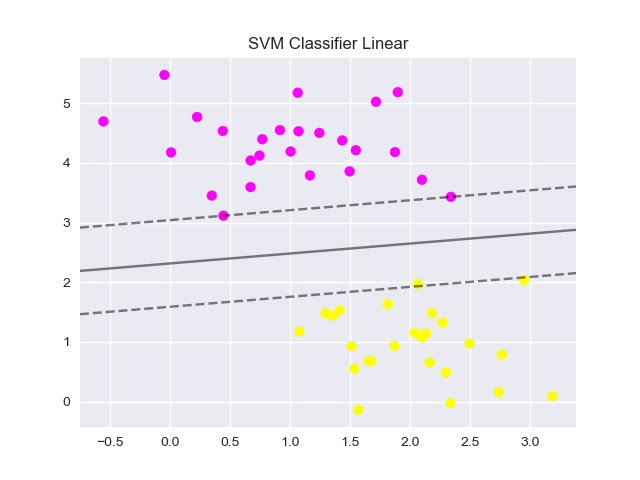
\includegraphics{assignment/svm/svc_lr.png}
\caption{}
\end{figure}

    \begin{figure}
\centering
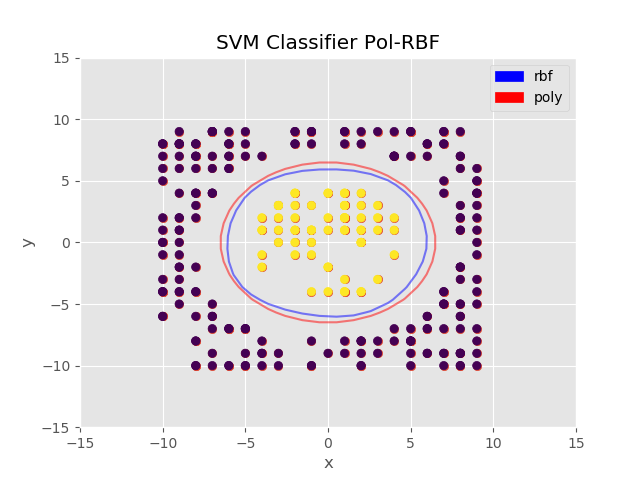
\includegraphics{assignment/svm/svc_pol.png}
\caption{}
\end{figure}

    \#

LR (Logisitic Regeression)

\begin{center}\rule{0.5\linewidth}{\linethickness}\end{center}

\textbf{任务} : 对线性/非线性可分不同类别的点进行多分类 ****
\textbf{类型} : 监督学习

\textbf{模型} : 3层fc nn, output layer(softmax) :
\({y_i} = \frac{{{e^{w{x_n} + b}}}}{{\sum\limits_{i = 1}^C {{e^{w{x_i} + b}}} }}\)

\textbf{评价方法} :
\(- \sum\limits_{i = 1}^N {{y_i}\log \frac{{{e^{w{x_i} + b}}}}{{\sum\limits_{j = 1}^C {{e^{w{x_j} + b}}} }}}\)

\textbf{优化方法} : Gradient Descent/SGD/ADAM/Adagrad/RMSprop

\begin{figure}
\centering
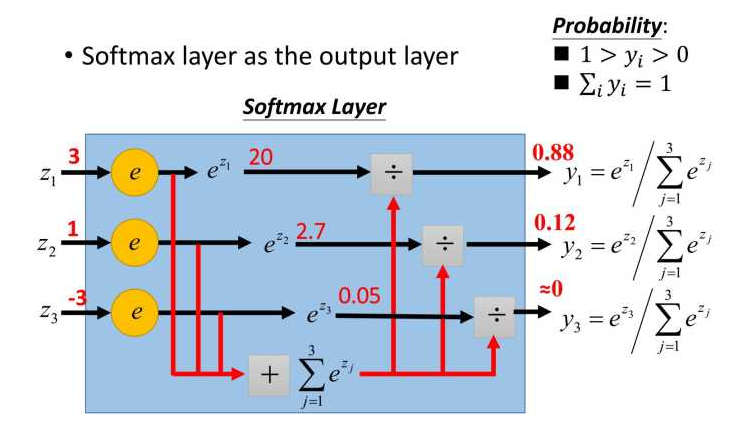
\includegraphics{softmax.png}
\caption{}
\end{figure}

    \begin{figure}
\centering
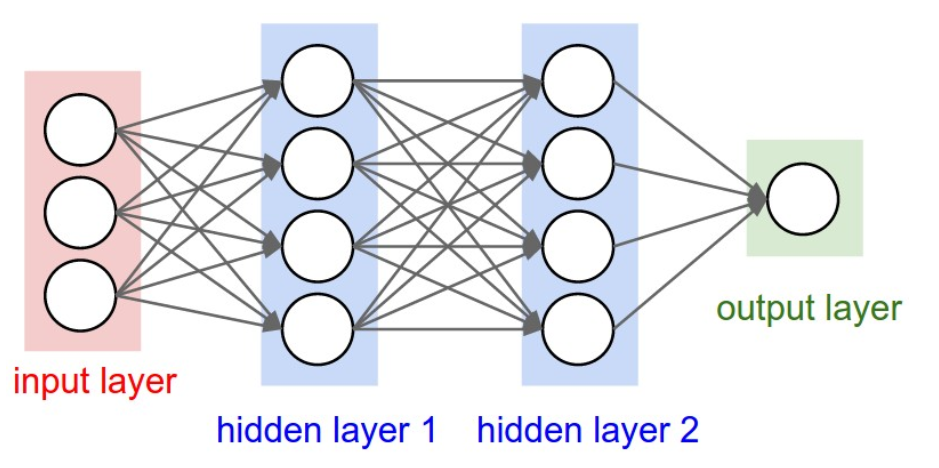
\includegraphics{bp.png}
\caption{}
\end{figure}

    \begin{figure}
\centering
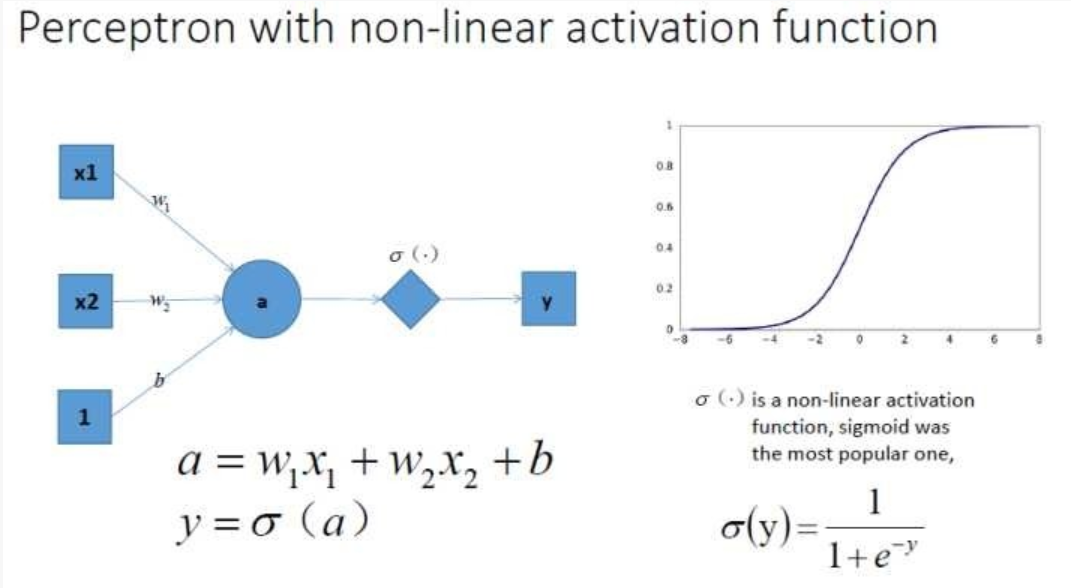
\includegraphics{node.png}
\caption{}
\end{figure}

    \begin{figure}
\centering
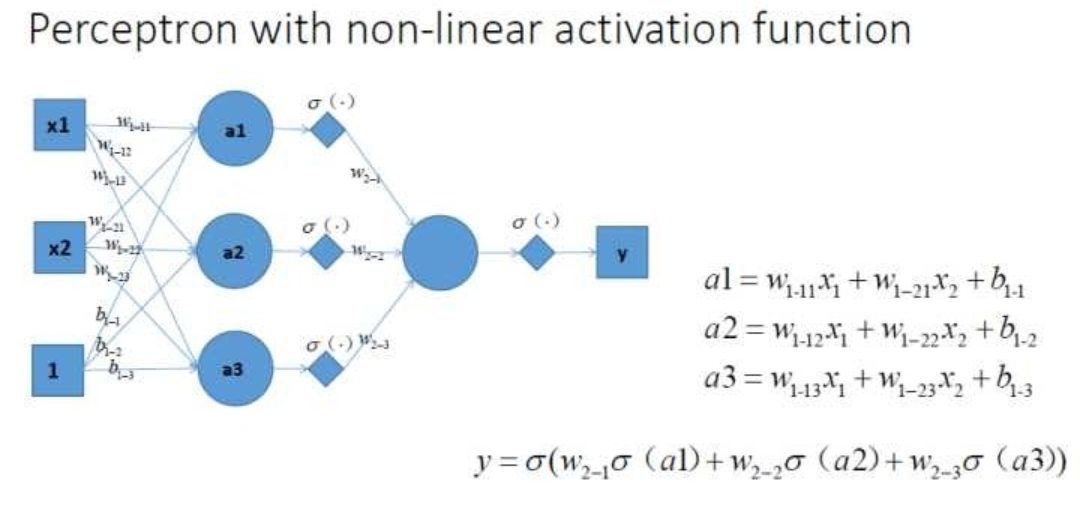
\includegraphics{multi-node.png}
\caption{}
\end{figure}

    \begin{figure}
\centering
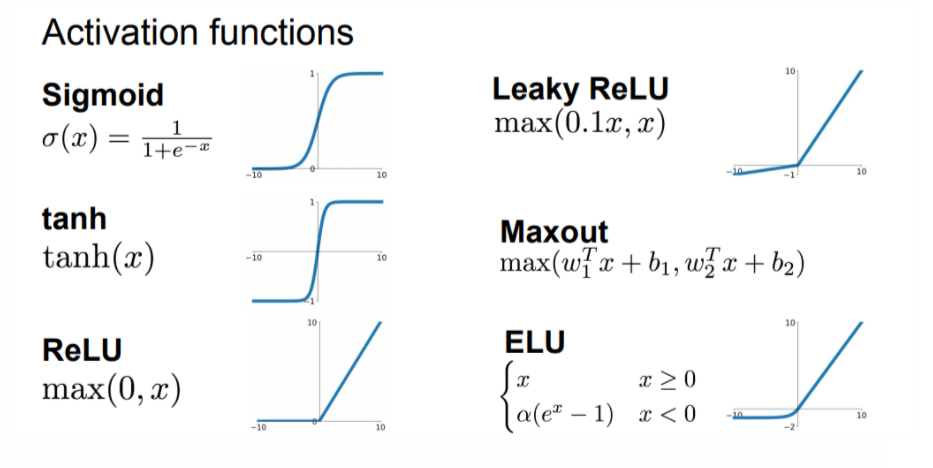
\includegraphics{active_function.png}
\caption{}
\end{figure}

    \begin{figure}
\centering
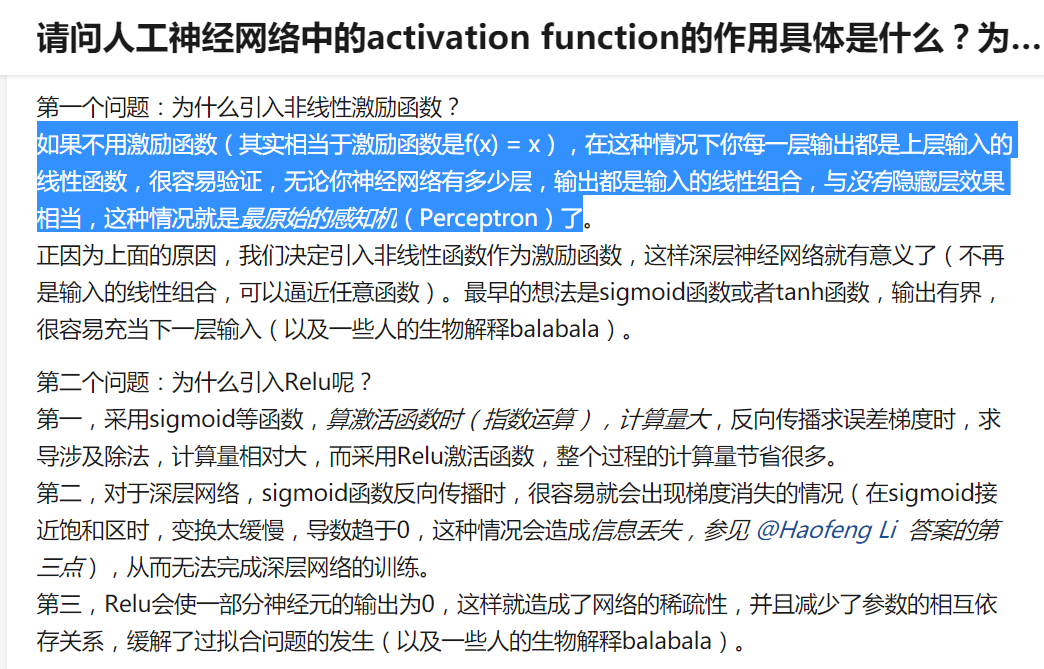
\includegraphics{activation.png}
\caption{}
\end{figure}

    \begin{figure}
\centering
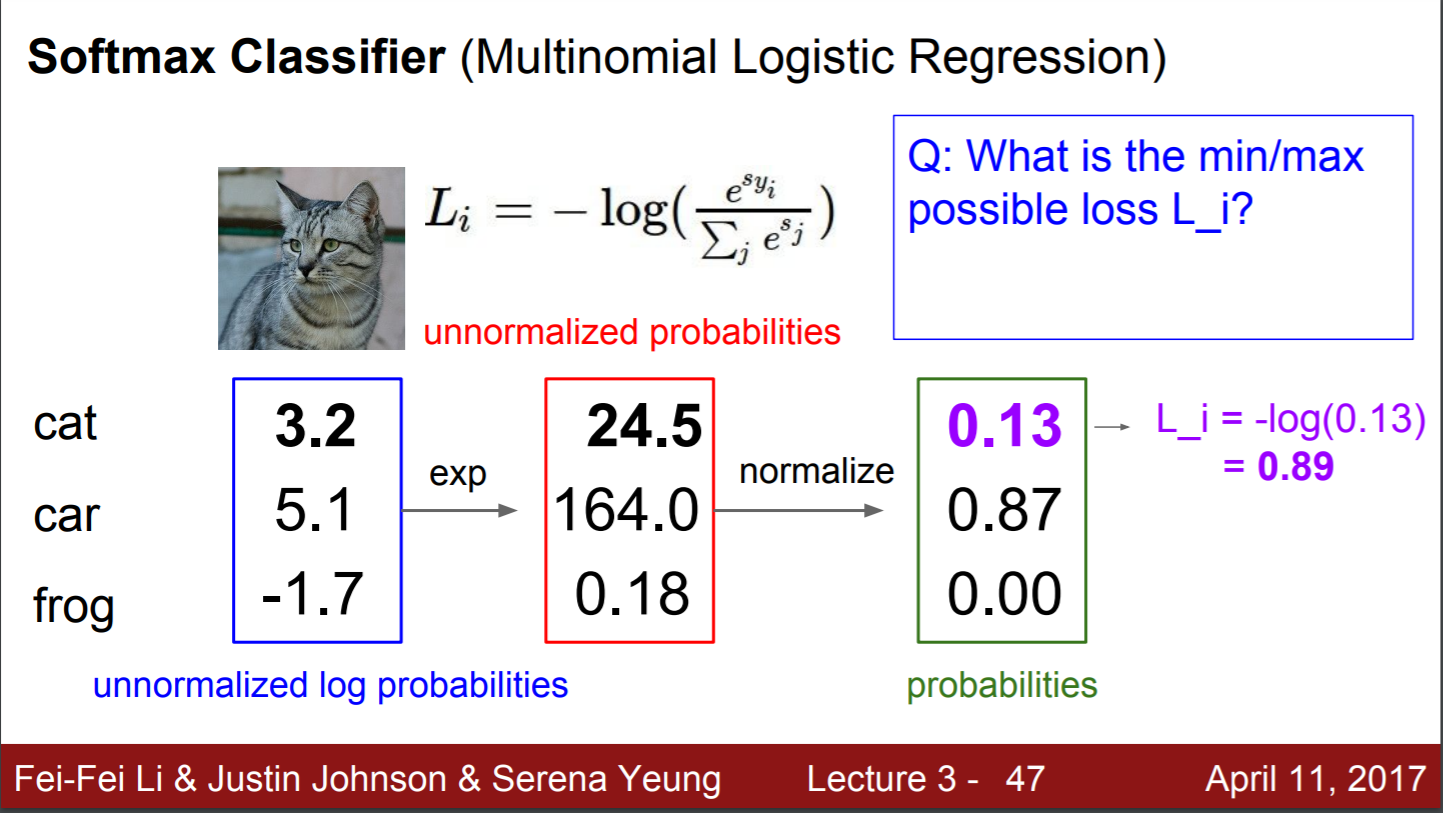
\includegraphics{loss.png}
\caption{}
\end{figure}

    \#

Gradient Descent

\begin{figure}
\centering
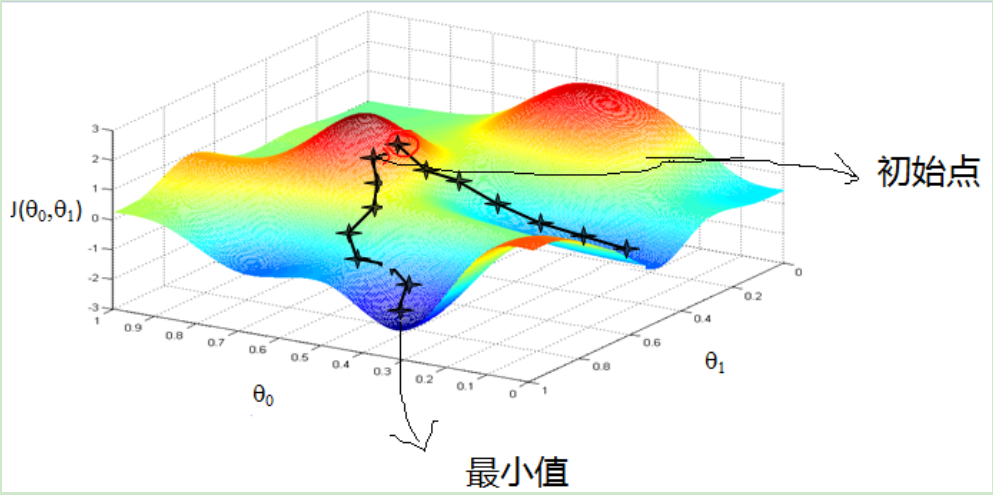
\includegraphics{gradient_descent.png}
\caption{}
\end{figure}

    \#

\({\theta _{\rm{j}}} = {\theta _j} - \alpha \frac{\partial }{{\partial {\theta _j}}}J(\theta )\)

\begin{figure}
\centering
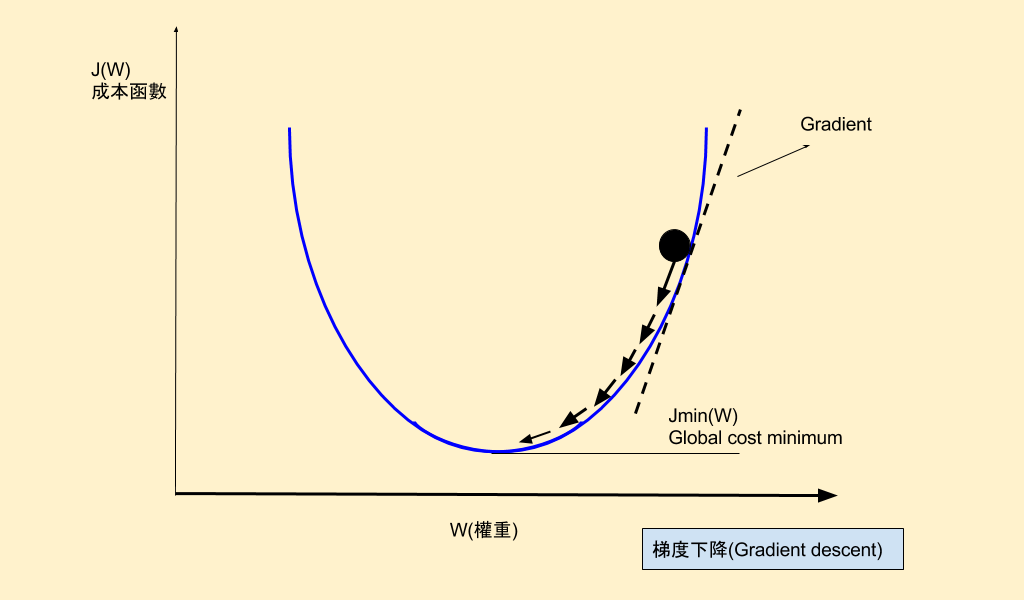
\includegraphics{_gradient_descent.png}
\caption{}
\end{figure}

    \#

Backpropagation

\begin{figure}
\centering
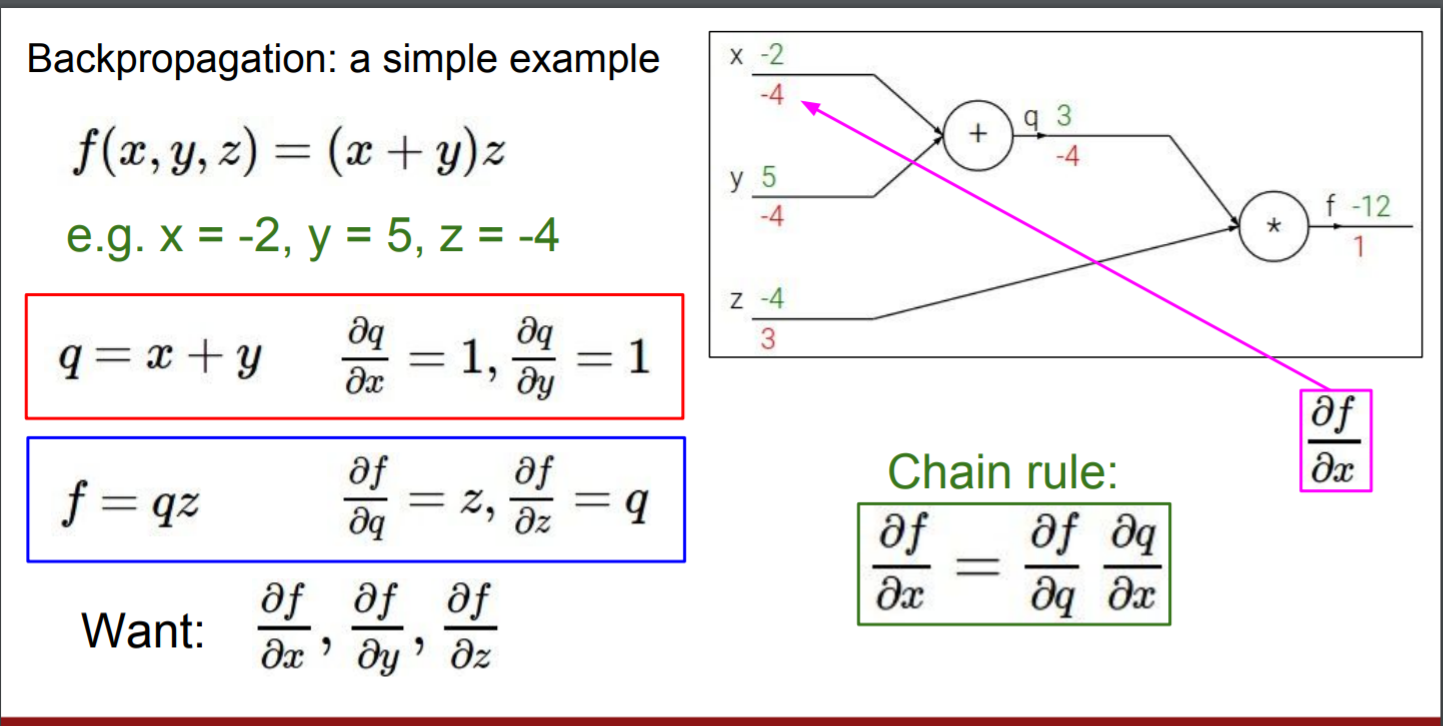
\includegraphics{backprop.png}
\caption{}
\end{figure}

    \begin{figure}
\centering
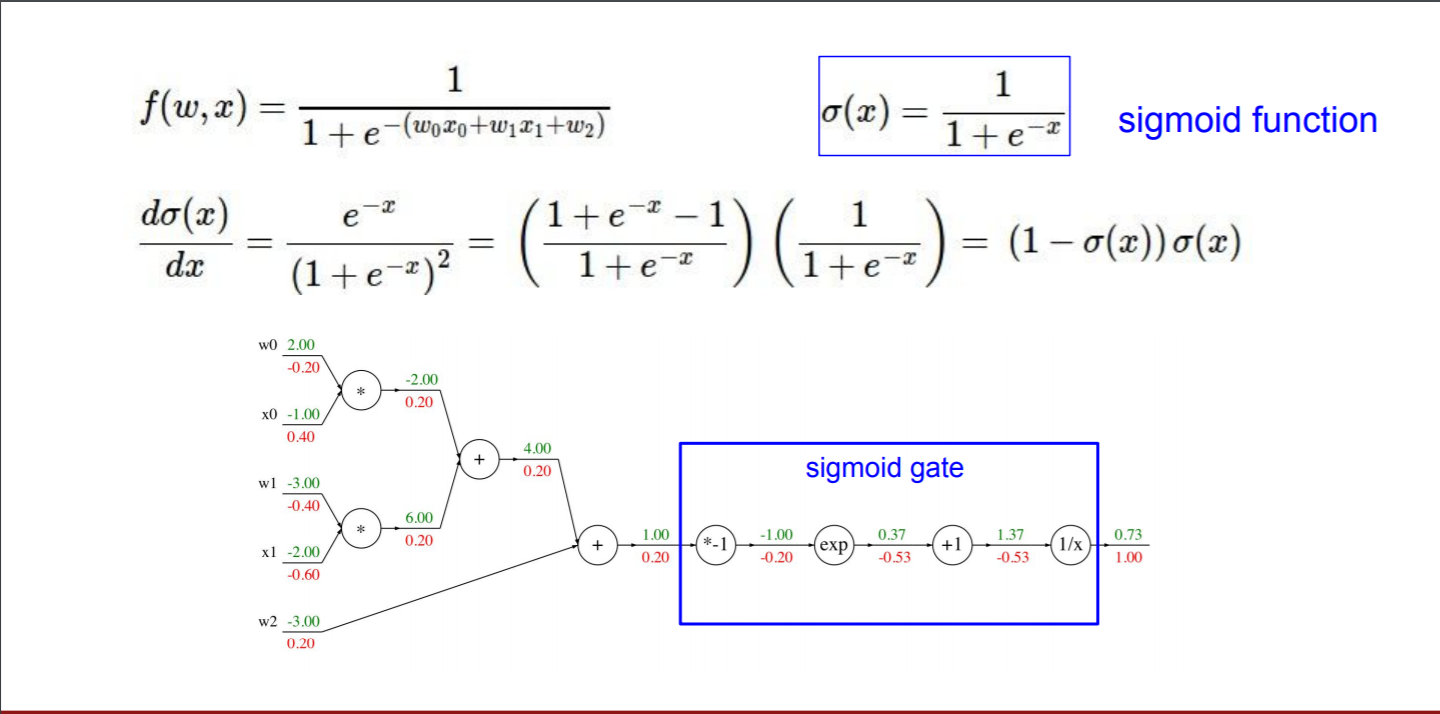
\includegraphics{sigmoid_backprop.png}
\caption{}
\end{figure}

    \#

Gradient Descent各算法对比

https://zhuanlan.zhihu.com/p/32230623

\begin{figure}
\centering
\includegraphics{_adag.gif}
\caption{}
\end{figure}

    \begin{Verbatim}[commandchars=\\\{\}]
{\color{incolor}In [{\color{incolor}1}]:} \PY{k+kn}{import} \PY{n+nn}{numpy} \PY{k}{as} \PY{n+nn}{np}
        \PY{k+kn}{import} \PY{n+nn}{tensorflow} \PY{k}{as} \PY{n+nn}{tf}
        \PY{k+kn}{import} \PY{n+nn}{matplotlib}\PY{n+nn}{.}\PY{n+nn}{pyplot} \PY{k}{as} \PY{n+nn}{plt}
        \PY{k+kn}{from} \PY{n+nn}{sklearn}\PY{n+nn}{.}\PY{n+nn}{datasets}\PY{n+nn}{.}\PY{n+nn}{samples\PYZus{}generator} \PY{k}{import} \PY{n}{make\PYZus{}blobs}
        \PY{k+kn}{import} \PY{n+nn}{time}
        \PY{k+kn}{import} \PY{n+nn}{os}
        \PY{n}{os}\PY{o}{.}\PY{n}{environ}\PY{p}{[}\PY{l+s+s1}{\PYZsq{}}\PY{l+s+s1}{TF\PYZus{}CPP\PYZus{}MIN\PYZus{}LOG\PYZus{}LEVEL}\PY{l+s+s1}{\PYZsq{}}\PY{p}{]}\PY{o}{=}\PY{l+s+s1}{\PYZsq{}}\PY{l+s+s1}{2}\PY{l+s+s1}{\PYZsq{}}
        
        \PY{n}{DIMENSION} \PY{o}{=} \PY{l+m+mi}{2}
        \PY{n}{KNUM} \PY{o}{=} \PY{l+m+mi}{4}
        \PY{n}{SAMPLE\PYZus{}CNT} \PY{o}{=} \PY{l+m+mi}{240}
        
        \PY{k}{def} \PY{n+nf}{init\PYZus{}variable}\PY{p}{(}\PY{n}{name}\PY{p}{,} \PY{n}{shape}\PY{p}{)}\PY{p}{:}
            \PY{k}{return}\PY{p}{(}\PY{n}{tf}\PY{o}{.}\PY{n}{get\PYZus{}variable}\PY{p}{(}\PY{n}{name}\PY{p}{,} \PY{n}{shape}\PY{o}{=}\PY{n}{shape}\PY{p}{,} \PY{n}{initializer}\PY{o}{=}\PY{n}{tf}\PY{o}{.}\PY{n}{contrib}\PY{o}{.}\PY{n}{layers}\PY{o}{.}\PY{n}{xavier\PYZus{}initializer}\PY{p}{(}\PY{p}{)}\PY{p}{)}\PY{p}{)}
                
        \PY{c+c1}{\PYZsh{} 测试数据生成}
        \PY{n}{x\PYZus{}data}\PY{p}{,} \PY{n}{y\PYZus{}data} \PY{o}{=} \PY{n}{make\PYZus{}blobs}\PY{p}{(}\PY{n}{n\PYZus{}samples}\PY{o}{=}\PY{n}{SAMPLE\PYZus{}CNT}\PY{p}{,} \PY{n}{n\PYZus{}features}\PY{o}{=}\PY{n}{DIMENSION}\PY{p}{,} \PY{n}{centers}\PY{o}{=}\PY{n}{KNUM}\PY{p}{,} \PY{n}{center\PYZus{}box}\PY{o}{=}\PY{p}{(}\PY{o}{\PYZhy{}}\PY{l+m+mi}{20}\PY{p}{,} \PY{l+m+mi}{20}\PY{p}{)}\PY{p}{,} \PY{n}{cluster\PYZus{}std}\PY{o}{=}\PY{l+m+mf}{1.5}\PY{p}{)}
        \PY{n}{x} \PY{o}{=} \PY{n}{x\PYZus{}data}\PY{o}{.}\PY{n}{tolist}\PY{p}{(}\PY{p}{)}
        \PY{n}{label}\PY{o}{=}\PY{n}{np}\PY{o}{.}\PY{n}{zeros}\PY{p}{(}\PY{p}{(}\PY{n}{SAMPLE\PYZus{}CNT}\PY{p}{,} \PY{n}{KNUM}\PY{p}{)}\PY{p}{)}
        
        \PY{n}{label}\PY{p}{[}\PY{n}{y\PYZus{}data}\PY{o}{==}\PY{l+m+mi}{0}\PY{p}{]} \PY{o}{=} \PY{p}{[}\PY{l+m+mi}{0}\PY{p}{,}\PY{l+m+mi}{0}\PY{p}{,}\PY{l+m+mi}{0}\PY{p}{,}\PY{l+m+mi}{1}\PY{p}{]}
        \PY{n}{label}\PY{p}{[}\PY{n}{y\PYZus{}data}\PY{o}{==}\PY{l+m+mi}{1}\PY{p}{]} \PY{o}{=} \PY{p}{[}\PY{l+m+mi}{0}\PY{p}{,}\PY{l+m+mi}{0}\PY{p}{,}\PY{l+m+mi}{1}\PY{p}{,}\PY{l+m+mi}{0}\PY{p}{]}
        \PY{n}{label}\PY{p}{[}\PY{n}{y\PYZus{}data}\PY{o}{==}\PY{l+m+mi}{2}\PY{p}{]} \PY{o}{=} \PY{p}{[}\PY{l+m+mi}{0}\PY{p}{,}\PY{l+m+mi}{1}\PY{p}{,}\PY{l+m+mi}{0}\PY{p}{,}\PY{l+m+mi}{0}\PY{p}{]}
        \PY{n}{label}\PY{p}{[}\PY{n}{y\PYZus{}data}\PY{o}{==}\PY{l+m+mi}{3}\PY{p}{]} \PY{o}{=} \PY{p}{[}\PY{l+m+mi}{1}\PY{p}{,}\PY{l+m+mi}{0}\PY{p}{,}\PY{l+m+mi}{0}\PY{p}{,}\PY{l+m+mi}{0}\PY{p}{]}
        
        \PY{n}{y} \PY{o}{=} \PY{n}{label}\PY{o}{.}\PY{n}{tolist}\PY{p}{(}\PY{p}{)}
        \PY{n}{keep\PYZus{}prob} \PY{o}{=} \PY{n}{tf}\PY{o}{.}\PY{n}{placeholder}\PY{p}{(}\PY{n}{tf}\PY{o}{.}\PY{n}{float32}\PY{p}{)}
        \PY{n}{prediction\PYZus{}value} \PY{o}{=} \PY{n}{y}\PY{o}{.}\PY{n}{copy}\PY{p}{(}\PY{p}{)}
        
        \PY{c+c1}{\PYZsh{} 生成学习网络}
        \PY{c+c1}{\PYZsh{} layer0: input}
        \PY{n}{xs} \PY{o}{=} \PY{n}{tf}\PY{o}{.}\PY{n}{placeholder}\PY{p}{(}\PY{l+s+s2}{\PYZdq{}}\PY{l+s+s2}{float}\PY{l+s+s2}{\PYZdq{}}\PY{p}{,} \PY{p}{[}\PY{k+kc}{None}\PY{p}{,} \PY{l+m+mi}{2}\PY{p}{]}\PY{p}{)}
        \PY{n}{ys} \PY{o}{=} \PY{n}{tf}\PY{o}{.}\PY{n}{placeholder}\PY{p}{(}\PY{l+s+s2}{\PYZdq{}}\PY{l+s+s2}{float}\PY{l+s+s2}{\PYZdq{}}\PY{p}{,} \PY{p}{[}\PY{k+kc}{None}\PY{p}{,} \PY{l+m+mi}{4}\PY{p}{]}\PY{p}{)}
        \PY{n}{keep\PYZus{}prob} \PY{o}{=} \PY{n}{tf}\PY{o}{.}\PY{n}{placeholder}\PY{p}{(}\PY{n}{tf}\PY{o}{.}\PY{n}{float32}\PY{p}{)}
         
        \PY{c+c1}{\PYZsh{} layer1:}
        \PY{n}{W1} \PY{o}{=} \PY{n}{init\PYZus{}variable}\PY{p}{(}\PY{l+s+s1}{\PYZsq{}}\PY{l+s+s1}{W1}\PY{l+s+s1}{\PYZsq{}}\PY{p}{,} \PY{p}{[}\PY{l+m+mi}{2}\PY{p}{,}\PY{l+m+mi}{20}\PY{p}{]}\PY{p}{)}
        \PY{n}{bias1} \PY{o}{=} \PY{n}{init\PYZus{}variable}\PY{p}{(}\PY{l+s+s1}{\PYZsq{}}\PY{l+s+s1}{b1}\PY{l+s+s1}{\PYZsq{}}\PY{p}{,} \PY{p}{[}\PY{l+m+mi}{1}\PY{p}{,}\PY{l+m+mi}{20}\PY{p}{]}\PY{p}{)}
        \PY{n}{o1} \PY{o}{=} \PY{n}{tf}\PY{o}{.}\PY{n}{nn}\PY{o}{.}\PY{n}{relu}\PY{p}{(}\PY{n}{tf}\PY{o}{.}\PY{n}{matmul}\PY{p}{(}\PY{n}{xs}\PY{p}{,} \PY{n}{W1}\PY{p}{)} \PY{o}{+} \PY{n}{bias1}\PY{p}{)}
        \PY{n}{o1\PYZus{}drop} \PY{o}{=} \PY{n}{tf}\PY{o}{.}\PY{n}{nn}\PY{o}{.}\PY{n}{dropout}\PY{p}{(}\PY{n}{o1}\PY{p}{,} \PY{n}{keep\PYZus{}prob}\PY{p}{)}
        
        \PY{c+c1}{\PYZsh{} layer2:}
        \PY{n}{W2} \PY{o}{=} \PY{n}{init\PYZus{}variable}\PY{p}{(}\PY{l+s+s1}{\PYZsq{}}\PY{l+s+s1}{W2}\PY{l+s+s1}{\PYZsq{}}\PY{p}{,} \PY{p}{[}\PY{l+m+mi}{20}\PY{p}{,}\PY{l+m+mi}{20}\PY{p}{]}\PY{p}{)}
        \PY{n}{bias2} \PY{o}{=} \PY{n}{init\PYZus{}variable}\PY{p}{(}\PY{l+s+s1}{\PYZsq{}}\PY{l+s+s1}{b2}\PY{l+s+s1}{\PYZsq{}}\PY{p}{,} \PY{p}{[}\PY{l+m+mi}{1}\PY{p}{,}\PY{l+m+mi}{20}\PY{p}{]}\PY{p}{)}
        \PY{n}{o2} \PY{o}{=} \PY{n}{tf}\PY{o}{.}\PY{n}{nn}\PY{o}{.}\PY{n}{relu}\PY{p}{(}\PY{n}{tf}\PY{o}{.}\PY{n}{matmul}\PY{p}{(}\PY{n}{o1\PYZus{}drop}\PY{p}{,} \PY{n}{W2}\PY{p}{)} \PY{o}{+} \PY{n}{bias2}\PY{p}{)}
        \PY{n}{o2\PYZus{}drop} \PY{o}{=} \PY{n}{tf}\PY{o}{.}\PY{n}{nn}\PY{o}{.}\PY{n}{dropout}\PY{p}{(}\PY{n}{o2}\PY{p}{,} \PY{n}{keep\PYZus{}prob}\PY{p}{)}
        
        \PY{c+c1}{\PYZsh{} layer3: output}
        \PY{n}{W3} \PY{o}{=} \PY{n}{init\PYZus{}variable}\PY{p}{(}\PY{l+s+s1}{\PYZsq{}}\PY{l+s+s1}{W3}\PY{l+s+s1}{\PYZsq{}}\PY{p}{,} \PY{p}{[}\PY{l+m+mi}{20}\PY{p}{,}\PY{l+m+mi}{4}\PY{p}{]}\PY{p}{)}
        \PY{n}{bias3} \PY{o}{=} \PY{n}{init\PYZus{}variable}\PY{p}{(}\PY{l+s+s1}{\PYZsq{}}\PY{l+s+s1}{b3}\PY{l+s+s1}{\PYZsq{}}\PY{p}{,} \PY{p}{[}\PY{l+m+mi}{1}\PY{p}{,}\PY{l+m+mi}{4}\PY{p}{]}\PY{p}{)}
        \PY{c+c1}{\PYZsh{}predict = tf.nn.softmax(tf.matmul(o2\PYZus{}drop, W3) + bias3)}
        \PY{n}{o3} \PY{o}{=} \PY{n}{tf}\PY{o}{.}\PY{n}{matmul}\PY{p}{(}\PY{n}{o2\PYZus{}drop}\PY{p}{,} \PY{n}{W3}\PY{p}{)} \PY{o}{+} \PY{n}{bias3}
        \PY{n}{predict} \PY{o}{=} \PY{n}{tf}\PY{o}{.}\PY{n}{nn}\PY{o}{.}\PY{n}{softmax}\PY{p}{(}\PY{n}{o3}\PY{p}{)}
\end{Verbatim}


    \begin{Verbatim}[commandchars=\\\{\}]
D:\textbackslash{}cloud\textbackslash{}anaconda\textbackslash{}lib\textbackslash{}site-packages\textbackslash{}h5py\textbackslash{}\_\_init\_\_.py:34: FutureWarning: Conversion of the second argument of issubdtype from `float` to `np.floating` is deprecated. In future, it will be treated as `np.float64 == np.dtype(float).type`.
  from .\_conv import register\_converters as \_register\_converters

    \end{Verbatim}

    \begin{Verbatim}[commandchars=\\\{\}]
{\color{incolor}In [{\color{incolor}2}]:} \PY{c+c1}{\PYZsh{} loss  sum( y*log(predict) )}
        \PY{n}{loss} \PY{o}{=} \PY{n}{tf}\PY{o}{.}\PY{n}{reduce\PYZus{}mean}\PY{p}{(}\PY{n}{tf}\PY{o}{.}\PY{n}{nn}\PY{o}{.}\PY{n}{softmax\PYZus{}cross\PYZus{}entropy\PYZus{}with\PYZus{}logits}\PY{p}{(}\PY{n}{logits}\PY{o}{=}\PY{n}{o3}\PY{p}{,} \PY{n}{labels}\PY{o}{=}\PY{n}{ys}\PY{p}{)}\PY{p}{)}
        \PY{c+c1}{\PYZsh{}loss = tf.reduce\PYZus{}mean(\PYZhy{}tf.reduce\PYZus{}sum(ys*tf.log(predict), reduction\PYZus{}indices=[1]))}
        
        \PY{c+c1}{\PYZsh{} train method}
        \PY{c+c1}{\PYZsh{}train = tf.train.GradientDescentOptimizer(0.1).minimize(loss)}
        \PY{n}{train} \PY{o}{=} \PY{n}{tf}\PY{o}{.}\PY{n}{train}\PY{o}{.}\PY{n}{AdamOptimizer}\PY{p}{(}\PY{l+m+mf}{1e\PYZhy{}3}\PY{p}{)}\PY{o}{.}\PY{n}{minimize}\PY{p}{(}\PY{n}{loss}\PY{p}{)}
        
        \PY{c+c1}{\PYZsh{}init all variables, it will be activated by use sess.run(init)}
        \PY{n}{init} \PY{o}{=} \PY{n}{tf}\PY{o}{.}\PY{n}{global\PYZus{}variables\PYZus{}initializer}\PY{p}{(}\PY{p}{)}
        
        \PY{k}{with} \PY{n}{tf}\PY{o}{.}\PY{n}{Session}\PY{p}{(}\PY{p}{)} \PY{k}{as} \PY{n}{sess}\PY{p}{:}
            \PY{n}{sess}\PY{o}{.}\PY{n}{run}\PY{p}{(}\PY{n}{init}\PY{p}{)}
            \PY{k}{for} \PY{n}{i} \PY{o+ow}{in} \PY{n+nb}{range}\PY{p}{(}\PY{l+m+mi}{200}\PY{p}{)}\PY{p}{:}
                \PY{n}{sess}\PY{o}{.}\PY{n}{run}\PY{p}{(}\PY{n}{train}\PY{p}{,} \PY{n}{feed\PYZus{}dict}\PY{o}{=}\PY{p}{\PYZob{}}\PY{n}{xs}\PY{p}{:}\PY{n}{x}\PY{p}{,} \PY{n}{ys}\PY{p}{:}\PY{n}{y}\PY{p}{,} \PY{n}{keep\PYZus{}prob}\PY{p}{:} \PY{l+m+mf}{0.5}\PY{p}{\PYZcb{}}\PY{p}{)}
                \PY{k}{if} \PY{n}{i} \PY{o}{\PYZpc{}} \PY{l+m+mi}{10} \PY{o}{==} \PY{l+m+mi}{0}\PY{p}{:}
                    \PY{n}{prediction\PYZus{}value} \PY{o}{=} \PY{n}{sess}\PY{o}{.}\PY{n}{run}\PY{p}{(}\PY{n}{predict}\PY{p}{,} \PY{n}{feed\PYZus{}dict}\PY{o}{=}\PY{p}{\PYZob{}}\PY{n}{xs}\PY{p}{:}\PY{n}{x}\PY{p}{,} \PY{n}{keep\PYZus{}prob}\PY{p}{:} \PY{l+m+mi}{1}\PY{p}{\PYZcb{}}\PY{p}{)}
                    \PY{n+nb}{print}\PY{p}{(}\PY{n}{sess}\PY{o}{.}\PY{n}{run}\PY{p}{(}\PY{n}{loss}\PY{p}{,} \PY{n}{feed\PYZus{}dict}\PY{o}{=}\PY{p}{\PYZob{}}\PY{n}{xs}\PY{p}{:}\PY{n}{x}\PY{p}{,} \PY{n}{ys}\PY{p}{:}\PY{n}{y}\PY{p}{,} \PY{n}{keep\PYZus{}prob}\PY{p}{:} \PY{l+m+mi}{1}\PY{p}{\PYZcb{}}\PY{p}{)}\PY{p}{)}
\end{Verbatim}


    \begin{Verbatim}[commandchars=\\\{\}]
WARNING:tensorflow:From <ipython-input-2-cd5c0946c093>:2: softmax\_cross\_entropy\_with\_logits (from tensorflow.python.ops.nn\_ops) is deprecated and will be removed in a future version.
Instructions for updating:

Future major versions of TensorFlow will allow gradients to flow
into the labels input on backprop by default.

See tf.nn.softmax\_cross\_entropy\_with\_logits\_v2.

2.0771701
1.4298545
1.2080476
1.062615
0.9569904
0.8710387
0.8117963
0.7671517
0.7361572
0.71022105
0.6842088
0.6632282
0.6432349
0.63005894
0.6273728
0.6227281
0.6168578
0.61016667
0.60824126
0.60349876

    \end{Verbatim}

    \begin{figure}
\centering
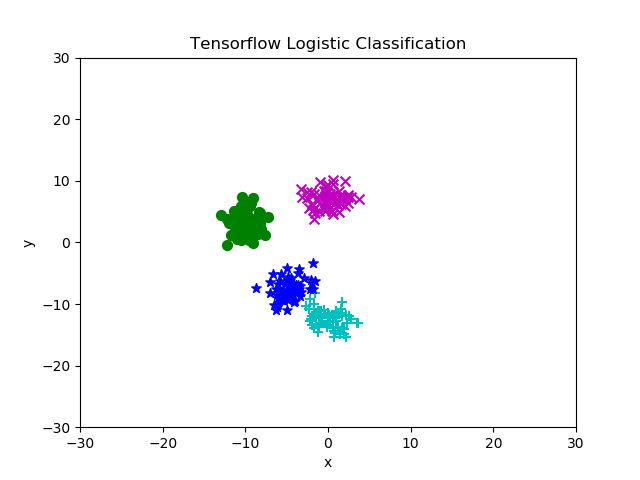
\includegraphics{assignment/lr/tf_mul_lc.gif}
\caption{}
\end{figure}

    \#

LR (Linear Regeression)

\begin{center}\rule{0.5\linewidth}{\linethickness}\end{center}

\textbf{任务} : 对一组数据进行曲线拟合 **** \textbf{类型} : 监督学习

\textbf{模型} : 2层fc nn, output layer : \({y_i} = w{x_i} + b\)

\textbf{评价方法} :
\(\sum\limits_{i = 1}^N {{{\left( {{{\rm{y}}_i} - (w{x_i} + b)} \right)}^2}}\)

\textbf{优化方法} : Gradient Descent/SGD/ADAM/Adagrad/RMSprop

    \begin{Verbatim}[commandchars=\\\{\}]
{\color{incolor}In [{\color{incolor}6}]:} \PY{k+kn}{import} \PY{n+nn}{numpy} \PY{k}{as} \PY{n+nn}{np}
        \PY{k+kn}{import} \PY{n+nn}{tensorflow} \PY{k}{as} \PY{n+nn}{tf}
        \PY{k+kn}{import} \PY{n+nn}{matplotlib}\PY{n+nn}{.}\PY{n+nn}{pyplot} \PY{k}{as} \PY{n+nn}{plt}
        \PY{k+kn}{import} \PY{n+nn}{time}
        \PY{k+kn}{import} \PY{n+nn}{os}
        \PY{n}{os}\PY{o}{.}\PY{n}{environ}\PY{p}{[}\PY{l+s+s1}{\PYZsq{}}\PY{l+s+s1}{TF\PYZus{}CPP\PYZus{}MIN\PYZus{}LOG\PYZus{}LEVEL}\PY{l+s+s1}{\PYZsq{}}\PY{p}{]}\PY{o}{=}\PY{l+s+s1}{\PYZsq{}}\PY{l+s+s1}{2}\PY{l+s+s1}{\PYZsq{}}
        
        \PY{c+c1}{\PYZsh{} 测试数据生成}
        \PY{n}{x\PYZus{}data} \PY{o}{=} \PY{n}{np}\PY{o}{.}\PY{n}{linspace}\PY{p}{(}\PY{o}{\PYZhy{}}\PY{l+m+mi}{1}\PY{p}{,} \PY{l+m+mi}{1}\PY{p}{,} \PY{l+m+mi}{300}\PY{p}{)}\PY{p}{[}\PY{p}{:}\PY{p}{,} \PY{n}{np}\PY{o}{.}\PY{n}{newaxis}\PY{p}{]}
        \PY{n}{noise} \PY{o}{=} \PY{n}{np}\PY{o}{.}\PY{n}{random}\PY{o}{.}\PY{n}{normal}\PY{p}{(}\PY{l+m+mi}{0}\PY{p}{,} \PY{l+m+mf}{0.05}\PY{p}{,} \PY{n}{x\PYZus{}data}\PY{o}{.}\PY{n}{shape}\PY{p}{)}
        \PY{n}{y\PYZus{}data} \PY{o}{=} \PY{n}{np}\PY{o}{.}\PY{n}{square}\PY{p}{(}\PY{n}{x\PYZus{}data}\PY{p}{)} \PY{o}{\PYZhy{}} \PY{l+m+mf}{0.5} \PY{o}{+} \PY{n}{noise}
        
        \PY{c+c1}{\PYZsh{} 生成学习网络}
        \PY{c+c1}{\PYZsh{} layer0: input}
        \PY{n}{xs} \PY{o}{=} \PY{n}{tf}\PY{o}{.}\PY{n}{placeholder}\PY{p}{(}\PY{n}{tf}\PY{o}{.}\PY{n}{float32}\PY{p}{,} \PY{p}{[}\PY{k+kc}{None}\PY{p}{,} \PY{l+m+mi}{1}\PY{p}{]}\PY{p}{)}
        \PY{n}{ys} \PY{o}{=} \PY{n}{tf}\PY{o}{.}\PY{n}{placeholder}\PY{p}{(}\PY{n}{tf}\PY{o}{.}\PY{n}{float32}\PY{p}{,} \PY{p}{[}\PY{k+kc}{None}\PY{p}{,} \PY{l+m+mi}{1}\PY{p}{]}\PY{p}{)}
        
        \PY{c+c1}{\PYZsh{} layer1:}
        \PY{n}{W1} \PY{o}{=} \PY{n}{tf}\PY{o}{.}\PY{n}{Variable}\PY{p}{(}\PY{n}{tf}\PY{o}{.}\PY{n}{random\PYZus{}normal}\PY{p}{(}\PY{p}{[}\PY{l+m+mi}{1}\PY{p}{,}\PY{l+m+mi}{10}\PY{p}{]}\PY{p}{)}\PY{p}{)}
        \PY{n}{bias1} \PY{o}{=} \PY{n}{tf}\PY{o}{.}\PY{n}{Variable}\PY{p}{(}\PY{n}{tf}\PY{o}{.}\PY{n}{zeros}\PY{p}{(}\PY{p}{[}\PY{l+m+mi}{1}\PY{p}{,} \PY{l+m+mi}{10}\PY{p}{]}\PY{p}{)} \PY{o}{+} \PY{l+m+mf}{0.1}\PY{p}{)}
        \PY{n}{o1} \PY{o}{=} \PY{n}{tf}\PY{o}{.}\PY{n}{nn}\PY{o}{.}\PY{n}{relu}\PY{p}{(}\PY{n}{tf}\PY{o}{.}\PY{n}{matmul}\PY{p}{(}\PY{n}{xs}\PY{p}{,} \PY{n}{W1}\PY{p}{)} \PY{o}{+} \PY{n}{bias1}\PY{p}{)}
        
        \PY{c+c1}{\PYZsh{} layer2: output}
        \PY{n}{W2} \PY{o}{=} \PY{n}{tf}\PY{o}{.}\PY{n}{Variable}\PY{p}{(}\PY{n}{tf}\PY{o}{.}\PY{n}{random\PYZus{}normal}\PY{p}{(}\PY{p}{[}\PY{l+m+mi}{10}\PY{p}{,}\PY{l+m+mi}{1}\PY{p}{]}\PY{p}{)}\PY{p}{)}
        \PY{n}{bias2} \PY{o}{=} \PY{n}{tf}\PY{o}{.}\PY{n}{Variable}\PY{p}{(}\PY{l+m+mf}{0.1}\PY{p}{)}
        \PY{n}{predict} \PY{o}{=} \PY{n}{tf}\PY{o}{.}\PY{n}{matmul}\PY{p}{(}\PY{n}{o1}\PY{p}{,} \PY{n}{W2}\PY{p}{)} \PY{o}{+} \PY{n}{bias2}
        
        \PY{c+c1}{\PYZsh{} loss}
        \PY{n}{loss} \PY{o}{=} \PY{n}{tf}\PY{o}{.}\PY{n}{reduce\PYZus{}mean}\PY{p}{(}\PY{n}{tf}\PY{o}{.}\PY{n}{reduce\PYZus{}sum}\PY{p}{(}\PY{n}{tf}\PY{o}{.}\PY{n}{square}\PY{p}{(}\PY{n}{ys} \PY{o}{\PYZhy{}} \PY{n}{predict}\PY{p}{)}\PY{p}{,}
                             \PY{n}{reduction\PYZus{}indices}\PY{o}{=}\PY{p}{[}\PY{l+m+mi}{1}\PY{p}{]}\PY{p}{)}\PY{p}{)}
        
        \PY{c+c1}{\PYZsh{} train method}
        \PY{n}{train} \PY{o}{=} \PY{n}{tf}\PY{o}{.}\PY{n}{train}\PY{o}{.}\PY{n}{GradientDescentOptimizer}\PY{p}{(}\PY{l+m+mf}{0.1}\PY{p}{)}\PY{o}{.}\PY{n}{minimize}\PY{p}{(}\PY{n}{loss}\PY{p}{)}
        
        \PY{c+c1}{\PYZsh{}init all variables, it will be activated by use sess.run(init)}
        \PY{n}{init} \PY{o}{=} \PY{n}{tf}\PY{o}{.}\PY{n}{global\PYZus{}variables\PYZus{}initializer}\PY{p}{(}\PY{p}{)}
        
        
        \PY{k}{with} \PY{n}{tf}\PY{o}{.}\PY{n}{Session}\PY{p}{(}\PY{p}{)} \PY{k}{as} \PY{n}{sess}\PY{p}{:}
            \PY{n}{sess}\PY{o}{.}\PY{n}{run}\PY{p}{(}\PY{n}{init}\PY{p}{)}
            \PY{k}{for} \PY{n}{i} \PY{o+ow}{in} \PY{n+nb}{range}\PY{p}{(}\PY{l+m+mi}{1000}\PY{p}{)}\PY{p}{:}
                \PY{n}{sess}\PY{o}{.}\PY{n}{run}\PY{p}{(}\PY{n}{train}\PY{p}{,} \PY{n}{feed\PYZus{}dict}\PY{o}{=}\PY{p}{\PYZob{}}\PY{n}{xs}\PY{p}{:}\PY{n}{x\PYZus{}data}\PY{p}{,} \PY{n}{ys}\PY{p}{:}\PY{n}{y\PYZus{}data}\PY{p}{\PYZcb{}}\PY{p}{)}
                \PY{k}{if} \PY{n}{i} \PY{o}{\PYZpc{}} \PY{l+m+mi}{100} \PY{o}{==} \PY{l+m+mi}{0}\PY{p}{:}
                    \PY{n}{prediction\PYZus{}value} \PY{o}{=} \PY{n}{sess}\PY{o}{.}\PY{n}{run}\PY{p}{(}\PY{n}{predict}\PY{p}{,} \PY{n}{feed\PYZus{}dict}\PY{o}{=}\PY{p}{\PYZob{}}\PY{n}{xs}\PY{p}{:}\PY{n}{x\PYZus{}data}\PY{p}{\PYZcb{}}\PY{p}{)}
                    \PY{n+nb}{print}\PY{p}{(}\PY{n}{sess}\PY{o}{.}\PY{n}{run}\PY{p}{(}\PY{n}{loss}\PY{p}{,} \PY{n}{feed\PYZus{}dict}\PY{o}{=}\PY{p}{\PYZob{}}\PY{n}{xs}\PY{p}{:}\PY{n}{x\PYZus{}data}\PY{p}{,} \PY{n}{ys}\PY{p}{:}\PY{n}{y\PYZus{}data}\PY{p}{\PYZcb{}}\PY{p}{)}\PY{p}{)}
\end{Verbatim}


    \begin{Verbatim}[commandchars=\\\{\}]
0.21007633
0.009326225
0.0065052332
0.0041997177
0.0037967209
0.003648324
0.0035490533
0.0034687535
0.003410836
0.0033446297

    \end{Verbatim}

    \begin{figure}
\centering
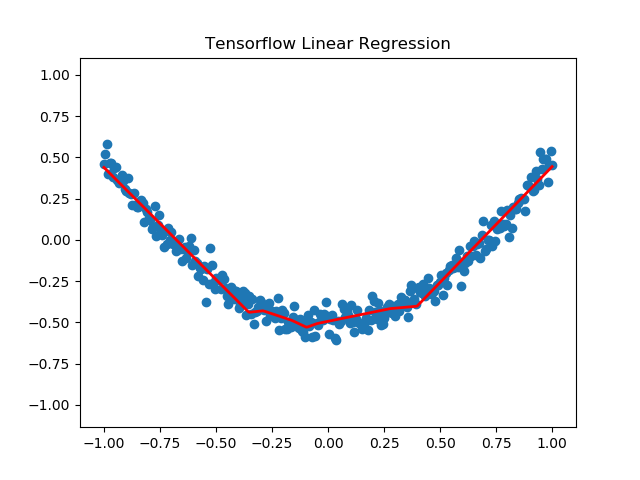
\includegraphics{assignment/lr/tf_lr.gif}
\caption{}
\end{figure}

    \#

KMEANS

\begin{center}\rule{0.5\linewidth}{\linethickness}\end{center}

\textbf{任务} : 对未标记的点进行多分类 **** \textbf{类型} : 非监督学习

\textbf{模型} :
\({y_j} - > \min \sum\limits_{i = 1}^K {{{({x_j} - {k_i})}^2}}\)

\textbf{评价方法} :
\(\sum\limits_{i = 1}^K {\sum\limits_{j = 1}^N {{{({x_j} - {k_i})}^2}} }\)

\textbf{优化方法} :
\({k_j} - > \frac{1}{N}\sum\limits_{i = 1}^N {{x_i} \bullet ({y_i} = = j)}\)

    \begin{center}\rule{0.5\linewidth}{\linethickness}\end{center}

\#

KMEANS Algorithm

\begin{longtable}[]{@{}l@{}}
\toprule
- \textbf{Input}: data
(\(T = \{x_{0}, x_{1}, ..., x_{i}\}\))\tabularnewline
- \textbf{Output}: \(\{y_{0}, y_{1}, ..., y_{i}\}\)\tabularnewline
- init \(\{k_{0}, k_{1}, ..., k_{K}\} \rightarrow x_{random}\) (s.t.
kmeans cluster cnt: K)\tabularnewline
- update \(y_{i} \rightarrow minarg\{(x_{i} - k)^2\}\)\tabularnewline
-
\(loss_{min}, loss_{cur}, loss_{pre} \leftarrow \sum\limits_i^K {\sum\limits_j^{y = = i} {{{({x_j} - {k_i})}^2}} }\)\tabularnewline
- for \(i= 0\rightarrow1000\) do\tabularnewline
- init \((w, b)\rightarrow random\) and
\(j\rightarrow 0\)\tabularnewline
- Save error label data to
\(T_{error} = \{(x_{0}, y_{0}), (x_{1}, y_{1}), ..., (x_{err}, y_{err})\}\)\tabularnewline
- while \(j != len(T_{error})\) do\tabularnewline
- \((\bar{w}, \bar{b}) \rightarrow (w, b) + y_{j}x_{j}\)\tabularnewline
- \(loss \leftarrow sum(sign(\bar{w}x + \bar{b}) != y)\)\tabularnewline
- if \(loss < loss_{min}\) then\tabularnewline
- break\tabularnewline
- end if\tabularnewline
- \(j=j+1\)\tabularnewline
- end while\tabularnewline
- if \(j != len(y_{err})\)\tabularnewline
- \((w_{best}, b_{best}) \leftarrow (\bar{w}, \bar{b})\)\tabularnewline
- \(loss_{min} \leftarrow loss\)\tabularnewline
- end if\tabularnewline
- j = 0\tabularnewline
- end for\tabularnewline
\bottomrule
\end{longtable}

    \begin{Verbatim}[commandchars=\\\{\}]
{\color{incolor}In [{\color{incolor}12}]:} \PY{k+kn}{import} \PY{n+nn}{numpy} \PY{k}{as} \PY{n+nn}{np}
         \PY{k+kn}{import} \PY{n+nn}{matplotlib}
         \PY{k+kn}{import} \PY{n+nn}{matplotlib}\PY{n+nn}{.}\PY{n+nn}{pyplot} \PY{k}{as} \PY{n+nn}{plt}
         \PY{k+kn}{from} \PY{n+nn}{sklearn}\PY{n+nn}{.}\PY{n+nn}{datasets}\PY{n+nn}{.}\PY{n+nn}{samples\PYZus{}generator} \PY{k}{import} \PY{n}{make\PYZus{}blobs}
         
         \PY{n}{DIMENSION} \PY{o}{=} \PY{l+m+mi}{2}
         \PY{n}{KNUM} \PY{o}{=} \PY{l+m+mi}{4}
         \PY{n}{SAMPLE\PYZus{}CNT} \PY{o}{=} \PY{l+m+mi}{240}
         \PY{n}{train\PYZus{}step} \PY{o}{=} \PY{l+m+mi}{100}
         
         
         \PY{k}{def} \PY{n+nf}{label\PYZus{}reset}\PY{p}{(}\PY{n}{x}\PY{p}{,} \PY{n}{kpoint}\PY{p}{)}\PY{p}{:}
             \PY{n}{\PYZus{}label} \PY{o}{=} \PY{n}{np}\PY{o}{.}\PY{n}{zeros}\PY{p}{(}\PY{p}{(}\PY{n}{x}\PY{o}{.}\PY{n}{shape}\PY{p}{[}\PY{l+m+mi}{0}\PY{p}{]}\PY{p}{,} \PY{l+m+mi}{1}\PY{p}{)}\PY{p}{)}
             \PY{k}{for} \PY{n}{i} \PY{o+ow}{in} \PY{n+nb}{range}\PY{p}{(}\PY{l+m+mi}{0}\PY{p}{,} \PY{n}{x}\PY{o}{.}\PY{n}{shape}\PY{p}{[}\PY{l+m+mi}{0}\PY{p}{]}\PY{p}{)}\PY{p}{:}
                 \PY{n}{\PYZus{}} \PY{o}{=} \PY{n}{np}\PY{o}{.}\PY{n}{linalg}\PY{o}{.}\PY{n}{norm}\PY{p}{(}\PY{n}{x}\PY{p}{[}\PY{n}{i}\PY{p}{,}\PY{p}{:}\PY{p}{]} \PY{o}{\PYZhy{}} \PY{n}{kpoint}\PY{p}{,} \PY{n}{axis}\PY{o}{=}\PY{l+m+mi}{1}\PY{p}{)}
                 \PY{n}{\PYZus{}label}\PY{p}{[}\PY{n}{i}\PY{p}{]} \PY{o}{=} \PY{n}{np}\PY{o}{.}\PY{n}{argmin}\PY{p}{(}\PY{n}{\PYZus{}}\PY{p}{,} \PY{l+m+mi}{0}\PY{p}{)}
          
             \PY{k}{return} \PY{n}{\PYZus{}label}
             
         
         \PY{k}{def} \PY{n+nf}{kpoint\PYZus{}reset}\PY{p}{(}\PY{n}{x}\PY{p}{,} \PY{n}{label}\PY{p}{)}\PY{p}{:}
             \PY{n}{\PYZus{}kpoint} \PY{o}{=} \PY{n}{np}\PY{o}{.}\PY{n}{zeros}\PY{p}{(}\PY{p}{(}\PY{n}{KNUM}\PY{p}{,} \PY{n}{DIMENSION}\PY{p}{)}\PY{p}{)}
             \PY{n}{idx} \PY{o}{=} \PY{l+m+mi}{0}
             \PY{k}{for} \PY{n}{i} \PY{o+ow}{in} \PY{n+nb}{range}\PY{p}{(}\PY{l+m+mi}{0}\PY{p}{,} \PY{n}{KNUM}\PY{p}{)}\PY{p}{:}
                 \PY{n}{idx} \PY{o}{=} \PY{n}{np}\PY{o}{.}\PY{n}{where}\PY{p}{(}\PY{n}{label}\PY{p}{[}\PY{p}{:}\PY{p}{,} \PY{l+m+mi}{0}\PY{p}{]} \PY{o}{==} \PY{n}{i}\PY{p}{)}
                 \PY{n}{\PYZus{}kpoint}\PY{p}{[}\PY{n}{i}\PY{p}{]} \PY{o}{=} \PY{n}{np}\PY{o}{.}\PY{n}{mean}\PY{p}{(}\PY{n}{x}\PY{p}{[}\PY{n}{idx}\PY{p}{]}\PY{p}{,} \PY{n}{axis}\PY{o}{=}\PY{l+m+mi}{0}\PY{p}{)}
             \PY{k}{return} \PY{n}{\PYZus{}kpoint}
         
         \PY{k}{def} \PY{n+nf}{cal\PYZus{}total}\PY{p}{(}\PY{n}{x}\PY{p}{,} \PY{n}{kpoint}\PY{p}{,} \PY{n}{label}\PY{p}{)}\PY{p}{:}
             \PY{n}{\PYZus{}sum} \PY{o}{=} \PY{l+m+mi}{0}
             \PY{k}{for} \PY{n}{i} \PY{o+ow}{in} \PY{n+nb}{range}\PY{p}{(}\PY{l+m+mi}{0}\PY{p}{,} \PY{n}{KNUM}\PY{p}{)}\PY{p}{:}
                 \PY{n}{idx} \PY{o}{=} \PY{n}{np}\PY{o}{.}\PY{n}{where}\PY{p}{(}\PY{n}{label}\PY{p}{[}\PY{p}{:}\PY{p}{,} \PY{l+m+mi}{0}\PY{p}{]} \PY{o}{==} \PY{n}{i}\PY{p}{)}
                 \PY{n}{\PYZus{}linalg} \PY{o}{=} \PY{n}{np}\PY{o}{.}\PY{n}{linalg}\PY{o}{.}\PY{n}{norm}\PY{p}{(}\PY{n}{x}\PY{p}{[}\PY{n}{idx}\PY{p}{]} \PY{o}{\PYZhy{}} \PY{n}{kpoint}\PY{p}{[}\PY{n}{i}\PY{p}{]}\PY{p}{,} \PY{n}{axis}\PY{o}{=}\PY{l+m+mi}{1}\PY{p}{)}
                 \PY{n}{\PYZus{}sum} \PY{o}{+}\PY{o}{=} \PY{n}{np}\PY{o}{.}\PY{n}{sum}\PY{p}{(}\PY{n}{\PYZus{}linalg}\PY{p}{)}
             \PY{n}{\PYZus{}sum} \PY{o}{/}\PY{o}{=} \PY{n}{SAMPLE\PYZus{}CNT}
             \PY{k}{return} \PY{n}{\PYZus{}sum}
         
         \PY{l+s+sd}{\PYZsq{}\PYZsq{}\PYZsq{}}
         \PY{l+s+sd}{\PYZsh{} x, y, label}
         \PY{l+s+sd}{x = np.zeros((SAMPLE\PYZus{}CNT, DIMENSION))}
         \PY{l+s+sd}{x = np.random.randint(\PYZhy{}20, 20, (SAMPLE\PYZus{}CNT, DIMENSION))}
         \PY{l+s+sd}{\PYZsq{}\PYZsq{}\PYZsq{}}
         \PY{n}{x}\PY{p}{,} \PY{n}{\PYZus{}} \PY{o}{=} \PY{n}{make\PYZus{}blobs}\PY{p}{(}\PY{n}{n\PYZus{}samples}\PY{o}{=}\PY{n}{SAMPLE\PYZus{}CNT}\PY{p}{,} \PY{n}{n\PYZus{}features}\PY{o}{=}\PY{n}{DIMENSION}\PY{p}{,} \PY{n}{centers}\PY{o}{=}\PY{n}{KNUM}\PY{p}{,} \PY{n}{center\PYZus{}box}\PY{o}{=}\PY{p}{(}\PY{o}{\PYZhy{}}\PY{l+m+mi}{20}\PY{p}{,} \PY{l+m+mi}{20}\PY{p}{)}\PY{p}{,} \PY{n}{cluster\PYZus{}std}\PY{o}{=}\PY{l+m+mf}{1.5}\PY{p}{)}
         
         \PY{n}{label} \PY{o}{=} \PY{n}{np}\PY{o}{.}\PY{n}{zeros}\PY{p}{(}\PY{p}{(}\PY{n}{SAMPLE\PYZus{}CNT}\PY{p}{,} \PY{l+m+mi}{1}\PY{p}{)}\PY{p}{)}
         
         \PY{c+c1}{\PYZsh{}kmeans init}
         \PY{n}{kpoint} \PY{o}{=} \PY{n}{np}\PY{o}{.}\PY{n}{random}\PY{o}{.}\PY{n}{randint}\PY{p}{(}\PY{o}{\PYZhy{}}\PY{l+m+mi}{20}\PY{p}{,} \PY{l+m+mi}{20}\PY{p}{,} \PY{p}{(}\PY{n}{KNUM}\PY{p}{,} \PY{n}{DIMENSION}\PY{p}{)}\PY{p}{)}
         \PY{n}{kpoint\PYZus{}min} \PY{o}{=} \PY{n}{kpoint}\PY{o}{.}\PY{n}{copy}\PY{p}{(}\PY{p}{)}
         
         \PY{n}{label} \PY{o}{=} \PY{n}{label\PYZus{}reset}\PY{p}{(}\PY{n}{x}\PY{p}{,} \PY{n}{kpoint}\PY{p}{)}
         \PY{n}{label\PYZus{}min} \PY{o}{=} \PY{n}{label}\PY{o}{.}\PY{n}{copy}\PY{p}{(}\PY{p}{)}
         
         \PY{n+nb}{sum} \PY{o}{=} \PY{n}{cal\PYZus{}total}\PY{p}{(}\PY{n}{x}\PY{p}{,} \PY{n}{kpoint}\PY{p}{,} \PY{n}{label}\PY{p}{)}
         \PY{n}{sum\PYZus{}min} \PY{o}{=} \PY{n+nb}{sum}
         \PY{n}{delta} \PY{o}{=} \PY{n+nb}{sum}
\end{Verbatim}


    \begin{Verbatim}[commandchars=\\\{\}]
{\color{incolor}In [{\color{incolor}13}]:} \PY{k}{for} \PY{n}{i} \PY{o+ow}{in} \PY{n+nb}{range}\PY{p}{(}\PY{n}{train\PYZus{}step}\PY{p}{)}\PY{p}{:}
             \PY{n}{kpoint} \PY{o}{=} \PY{n}{np}\PY{o}{.}\PY{n}{random}\PY{o}{.}\PY{n}{randint}\PY{p}{(}\PY{o}{\PYZhy{}}\PY{l+m+mi}{20}\PY{p}{,} \PY{l+m+mi}{20}\PY{p}{,} \PY{p}{(}\PY{n}{KNUM}\PY{p}{,} \PY{n}{DIMENSION}\PY{p}{)}\PY{p}{)}
             \PY{n}{label} \PY{o}{=} \PY{n}{label\PYZus{}reset}\PY{p}{(}\PY{n}{x}\PY{p}{,} \PY{n}{kpoint}\PY{p}{)}
             \PY{n+nb}{sum} \PY{o}{=} \PY{n}{cal\PYZus{}total}\PY{p}{(}\PY{n}{x}\PY{p}{,} \PY{n}{kpoint}\PY{p}{,} \PY{n}{label}\PY{p}{)}
             \PY{n}{delta} \PY{o}{=} \PY{n+nb}{sum}
             \PY{k}{while} \PY{n}{delta} \PY{o}{\PYZgt{}} \PY{l+m+mf}{0.001}\PY{p}{:}
                 \PY{n}{kpoint} \PY{o}{=} \PY{n}{kpoint\PYZus{}reset}\PY{p}{(}\PY{n}{x}\PY{p}{,} \PY{n}{label}\PY{p}{)}
                 \PY{n}{label} \PY{o}{=} \PY{n}{label\PYZus{}reset}\PY{p}{(}\PY{n}{x}\PY{p}{,} \PY{n}{kpoint}\PY{p}{)}
                 \PY{n}{\PYZus{}sum} \PY{o}{=} \PY{n}{cal\PYZus{}total}\PY{p}{(}\PY{n}{x}\PY{p}{,} \PY{n}{kpoint}\PY{p}{,} \PY{n}{label}\PY{p}{)}
                 \PY{n}{delta} \PY{o}{=} \PY{n+nb}{sum} \PY{o}{\PYZhy{}} \PY{n}{\PYZus{}sum}
                 \PY{n+nb}{sum} \PY{o}{=} \PY{n}{\PYZus{}sum}
                 \PY{c+c1}{\PYZsh{}print(\PYZdq{}sum: \PYZpc{}f\PYZdq{} \PYZpc{}sum)}
             \PY{k}{if} \PY{n+nb}{sum} \PY{o}{\PYZlt{}} \PY{n}{sum\PYZus{}min}\PY{p}{:}
                 \PY{n+nb}{print}\PY{p}{(}\PY{l+s+s2}{\PYZdq{}}\PY{l+s+s2}{Update sum\PYZus{}min: }\PY{l+s+si}{\PYZpc{}f}\PY{l+s+s2}{\PYZdq{}} \PY{o}{\PYZpc{}}\PY{k}{sum})
                 \PY{n}{sum\PYZus{}min} \PY{o}{=} \PY{n+nb}{sum}
                 \PY{n}{kpoint\PYZus{}min} \PY{o}{=} \PY{n}{kpoint}\PY{o}{.}\PY{n}{copy}\PY{p}{(}\PY{p}{)}
                 \PY{n}{label\PYZus{}min} \PY{o}{=} \PY{n}{label}\PY{o}{.}\PY{n}{copy}\PY{p}{(}\PY{p}{)}
         \PY{n+nb}{print}\PY{p}{(}\PY{n+nb}{sum}\PY{p}{)}
\end{Verbatim}


    \begin{Verbatim}[commandchars=\\\{\}]
Update sum\_min: 1.833920
Update sum\_min: 1.833920

    \end{Verbatim}

    \begin{Verbatim}[commandchars=\\\{\}]
D:\textbackslash{}cloud\textbackslash{}anaconda\textbackslash{}lib\textbackslash{}site-packages\textbackslash{}numpy\textbackslash{}core\textbackslash{}fromnumeric.py:2957: RuntimeWarning: Mean of empty slice.
  out=out, **kwargs)
D:\textbackslash{}cloud\textbackslash{}anaconda\textbackslash{}lib\textbackslash{}site-packages\textbackslash{}numpy\textbackslash{}core\textbackslash{}\_methods.py:73: RuntimeWarning: invalid value encountered in true\_divide
  ret, rcount, out=ret, casting='unsafe', subok=False)

    \end{Verbatim}

    \begin{Verbatim}[commandchars=\\\{\}]
1.8339197144463897

    \end{Verbatim}

    \begin{figure}
\centering
\includegraphics{assignment/kmeans/kmeans.gif}
\caption{}
\end{figure}

    \#

CNN

\begin{center}\rule{0.5\linewidth}{\linethickness}\end{center}

\textbf{任务} : OCR end-to-end 识别 **** \textbf{类型} : 监督学习

\textbf{模型} : 3层cnn + 3层relu + 2层fc, output layer(softmax) :
\({y_i} = \frac{{{e^{w{x_n} + b}}}}{{\sum\limits_{i = 1}^C {{e^{w{x_i} + b}}} }}\)

\textbf{评价方法} :
\(- \sum\limits_{i = 1}^N {{y_i}\log \frac{{{e^{w{x_i} + b}}}}{{\sum\limits_{j = 1}^C {{e^{w{x_j} + b}}} }}}\)

\textbf{优化方法} : Gradient Descent/SGD/ADAM/Adagrad/RMSprop

\begin{figure}
\centering
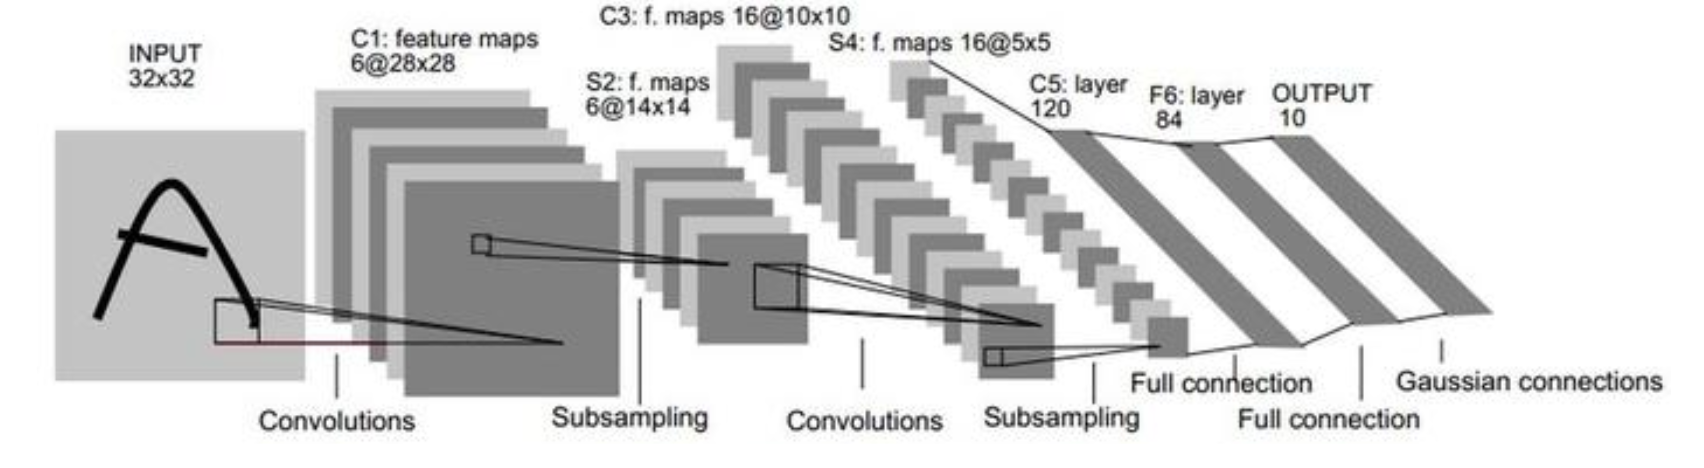
\includegraphics{lenet.png}
\caption{}
\end{figure}

    \#

Convolution

翻转-\textgreater{}移动-\textgreater{}乘积-\textgreater{}求和

\(f[x,y]*g[x,y] = \sum\limits_{{n_1} = - \infty }^\infty {\sum\limits_{{n_2} = - \infty }^\infty {f[{n_1},{n_2}]\bullet g[x - {n_1},y - {n_2}]} }\)
\includegraphics{conv.gif}

    \begin{Verbatim}[commandchars=\\\{\}]
{\color{incolor}In [{\color{incolor}22}]:} \PY{k+kn}{import} \PY{n+nn}{cv2}
         \PY{k+kn}{import} \PY{n+nn}{matplotlib}\PY{n+nn}{.}\PY{n+nn}{pyplot} \PY{k}{as} \PY{n+nn}{plt}
         \PY{k+kn}{import} \PY{n+nn}{numpy} \PY{k}{as} \PY{n+nn}{np}
         \PY{k+kn}{import} \PY{n+nn}{sys}
         \PY{o}{\PYZpc{}}\PY{k}{matplotlib} inline
         
         \PY{n}{img} \PY{o}{=} \PY{n}{np}\PY{o}{.}\PY{n}{ones}\PY{p}{(}\PY{p}{(}\PY{l+m+mi}{100}\PY{p}{,}\PY{l+m+mi}{100}\PY{p}{,}\PY{l+m+mi}{3}\PY{p}{)}\PY{p}{)}
         \PY{n}{img}\PY{p}{[}\PY{l+m+mi}{0}\PY{p}{:}\PY{l+m+mi}{20}\PY{p}{,}\PY{p}{:}\PY{p}{,}\PY{l+m+mi}{1}\PY{p}{]} \PY{o}{=} \PY{l+m+mi}{255}
         \PY{n}{img}\PY{p}{[}\PY{l+m+mi}{20}\PY{p}{:}\PY{l+m+mi}{40}\PY{p}{,}\PY{p}{:}\PY{p}{,}\PY{l+m+mi}{2}\PY{p}{]} \PY{o}{=} \PY{l+m+mi}{255}
         \PY{n}{img}\PY{p}{[}\PY{l+m+mi}{40}\PY{p}{:}\PY{l+m+mi}{100}\PY{p}{,}\PY{p}{:}\PY{p}{,}\PY{l+m+mi}{0}\PY{p}{]} \PY{o}{=} \PY{l+m+mi}{255}
         \PY{n}{img}\PY{p}{[}\PY{l+m+mi}{60}\PY{p}{:}\PY{l+m+mi}{80}\PY{p}{,}\PY{p}{:}\PY{p}{,}\PY{l+m+mi}{2}\PY{p}{]} \PY{o}{=} \PY{l+m+mi}{255}
         \PY{n}{img}\PY{p}{[}\PY{l+m+mi}{80}\PY{p}{:}\PY{l+m+mi}{100}\PY{p}{,}\PY{p}{:}\PY{p}{,}\PY{l+m+mi}{1}\PY{p}{]} \PY{o}{=} \PY{l+m+mi}{255}
         
         \PY{n}{prewitt} \PY{o}{=} \PY{n}{np}\PY{o}{.}\PY{n}{array}\PY{p}{(}\PY{p}{[}\PY{p}{[}\PY{o}{\PYZhy{}}\PY{l+m+mi}{1}\PY{p}{,}\PY{o}{\PYZhy{}}\PY{l+m+mi}{1}\PY{p}{,}\PY{o}{\PYZhy{}}\PY{l+m+mi}{1}\PY{p}{]}\PY{p}{,}
                   \PY{p}{[}\PY{l+m+mi}{0}\PY{p}{,}\PY{l+m+mi}{0}\PY{p}{,}\PY{l+m+mi}{0}\PY{p}{]}\PY{p}{,}
                   \PY{p}{[}\PY{l+m+mi}{1}\PY{p}{,}\PY{l+m+mi}{1}\PY{p}{,}\PY{l+m+mi}{1}\PY{p}{]}\PY{p}{]}\PY{p}{)}
         \PY{n}{res} \PY{o}{=} \PY{n}{cv2}\PY{o}{.}\PY{n}{filter2D}\PY{p}{(}\PY{n}{img}\PY{p}{,}\PY{o}{\PYZhy{}}\PY{l+m+mi}{1}\PY{p}{,}\PY{n}{prewitt}\PY{p}{)}
         \PY{n}{regular} \PY{o}{=} \PY{n}{np}\PY{o}{.}\PY{n}{uint8}\PY{p}{(}\PY{n}{res}\PY{p}{)}
         \PY{n+nb}{print}\PY{p}{(}\PY{n}{img}\PY{p}{[}\PY{l+m+mi}{19}\PY{p}{:}\PY{l+m+mi}{22}\PY{p}{,}\PY{l+m+mi}{19}\PY{p}{:}\PY{l+m+mi}{22}\PY{p}{,}\PY{l+m+mi}{1}\PY{p}{]}\PY{p}{)}
         \PY{n+nb}{print}\PY{p}{(}\PY{n}{res}\PY{p}{[}\PY{l+m+mi}{20}\PY{p}{,}\PY{l+m+mi}{20}\PY{p}{,}\PY{l+m+mi}{1}\PY{p}{]}\PY{p}{)}
         
         \PY{n}{plt}\PY{o}{.}\PY{n}{figure}\PY{p}{(}\PY{p}{)}
         \PY{n}{plt}\PY{o}{.}\PY{n}{subplot}\PY{p}{(}\PY{l+m+mi}{1}\PY{p}{,}\PY{l+m+mi}{2}\PY{p}{,}\PY{l+m+mi}{1}\PY{p}{)}
         \PY{n}{plt}\PY{o}{.}\PY{n}{imshow}\PY{p}{(}\PY{n}{img}\PY{p}{)}
         \PY{n}{plt}\PY{o}{.}\PY{n}{subplot}\PY{p}{(}\PY{l+m+mi}{1}\PY{p}{,}\PY{l+m+mi}{2}\PY{p}{,}\PY{l+m+mi}{2}\PY{p}{)}
         \PY{n}{plt}\PY{o}{.}\PY{n}{imshow}\PY{p}{(}\PY{n}{regular}\PY{p}{)}
         \PY{n}{plt}\PY{o}{.}\PY{n}{show}\PY{p}{(}\PY{p}{)}
\end{Verbatim}


    \begin{Verbatim}[commandchars=\\\{\}]
[[255. 255. 255.]
 [  1.   1.   1.]
 [  1.   1.   1.]]
-762.0

    \end{Verbatim}

    \begin{center}
    \adjustimage{max size={0.9\linewidth}{0.9\paperheight}}{ml_files/ml_46_1.png}
    \end{center}
    { \hspace*{\fill} \\}
    
    \#

LeNet、AlexNet、GoogLeNet、VGG、ResNet

\begin{figure}
\centering
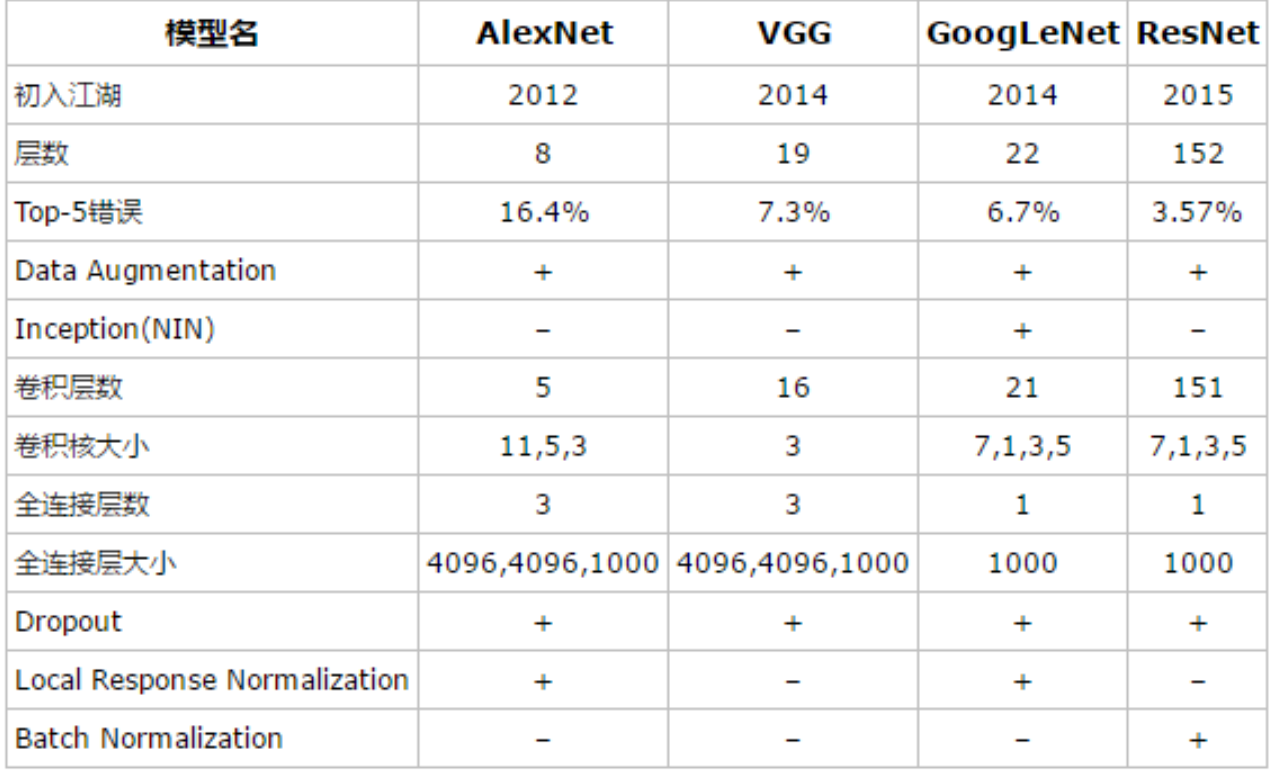
\includegraphics{net比较.png}
\caption{}
\end{figure}

    \begin{figure}
\centering
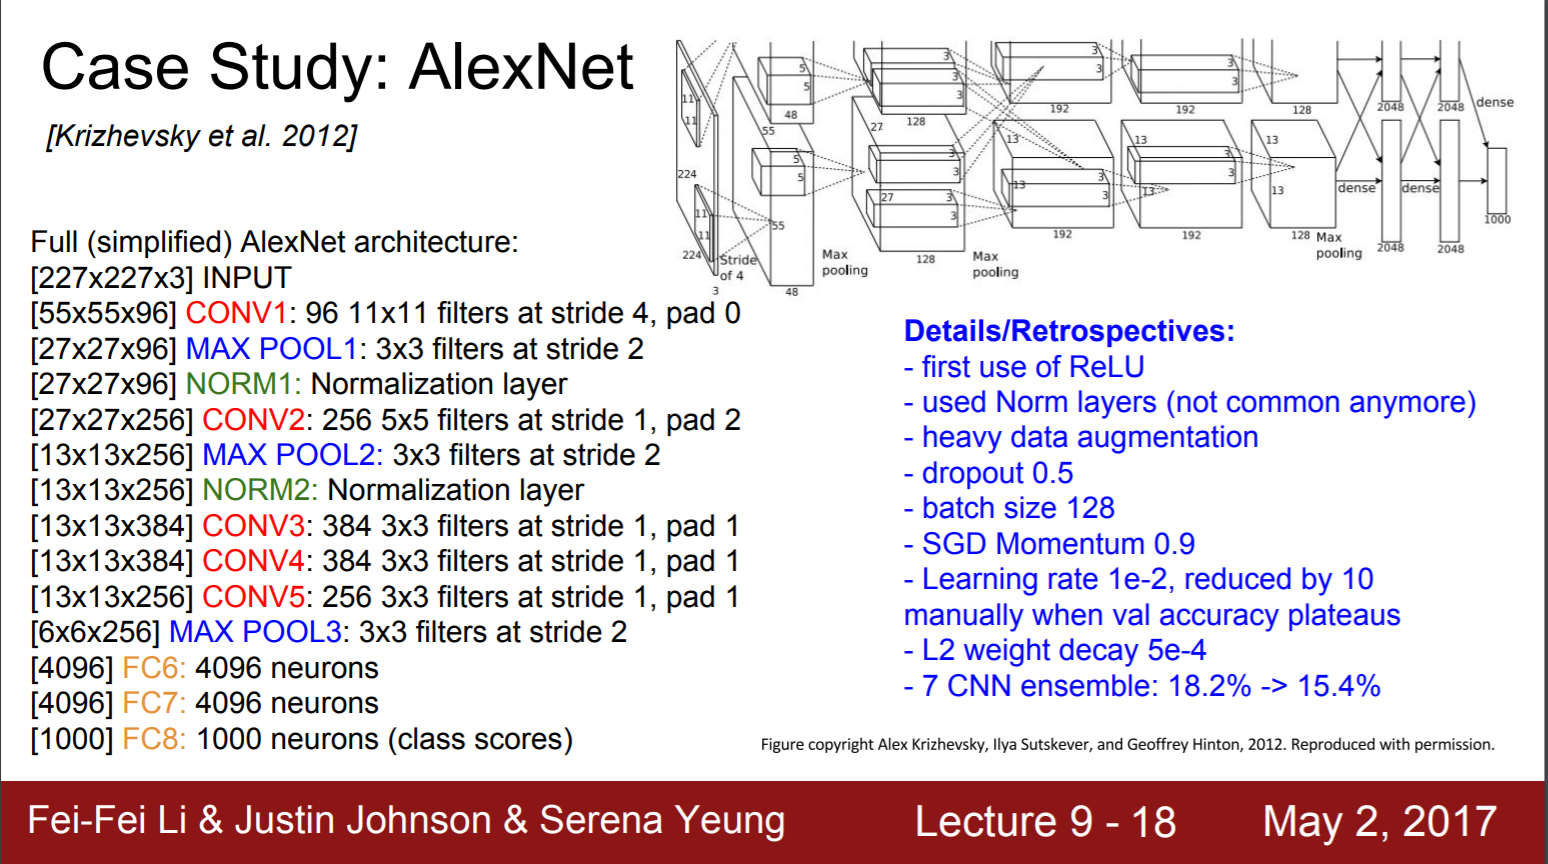
\includegraphics{alex_net.png}
\caption{}
\end{figure}

    \begin{figure}
\centering
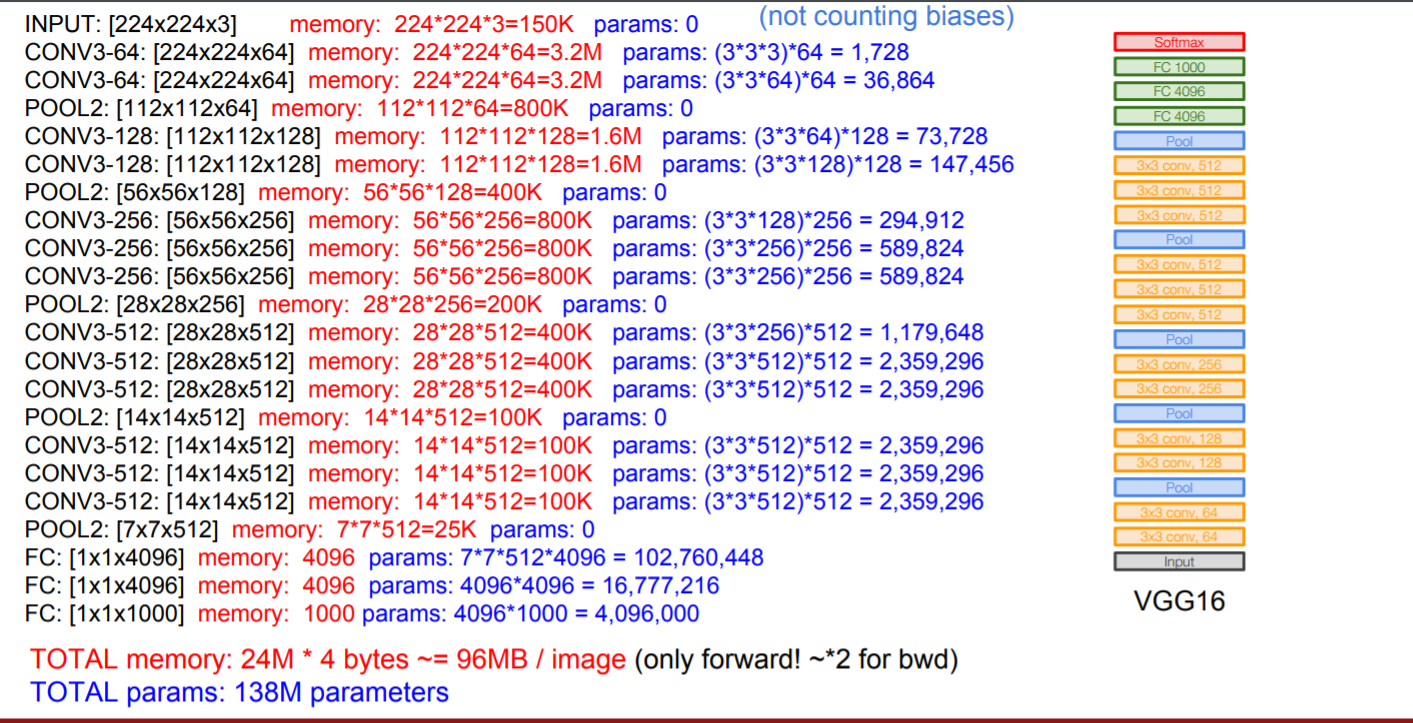
\includegraphics{vgg16_para.png}
\caption{}
\end{figure}

    \includegraphics{asamples.gif} \includegraphics{a384.gif}

    \#

Mask R-CNN Segment

\begin{figure}
\centering
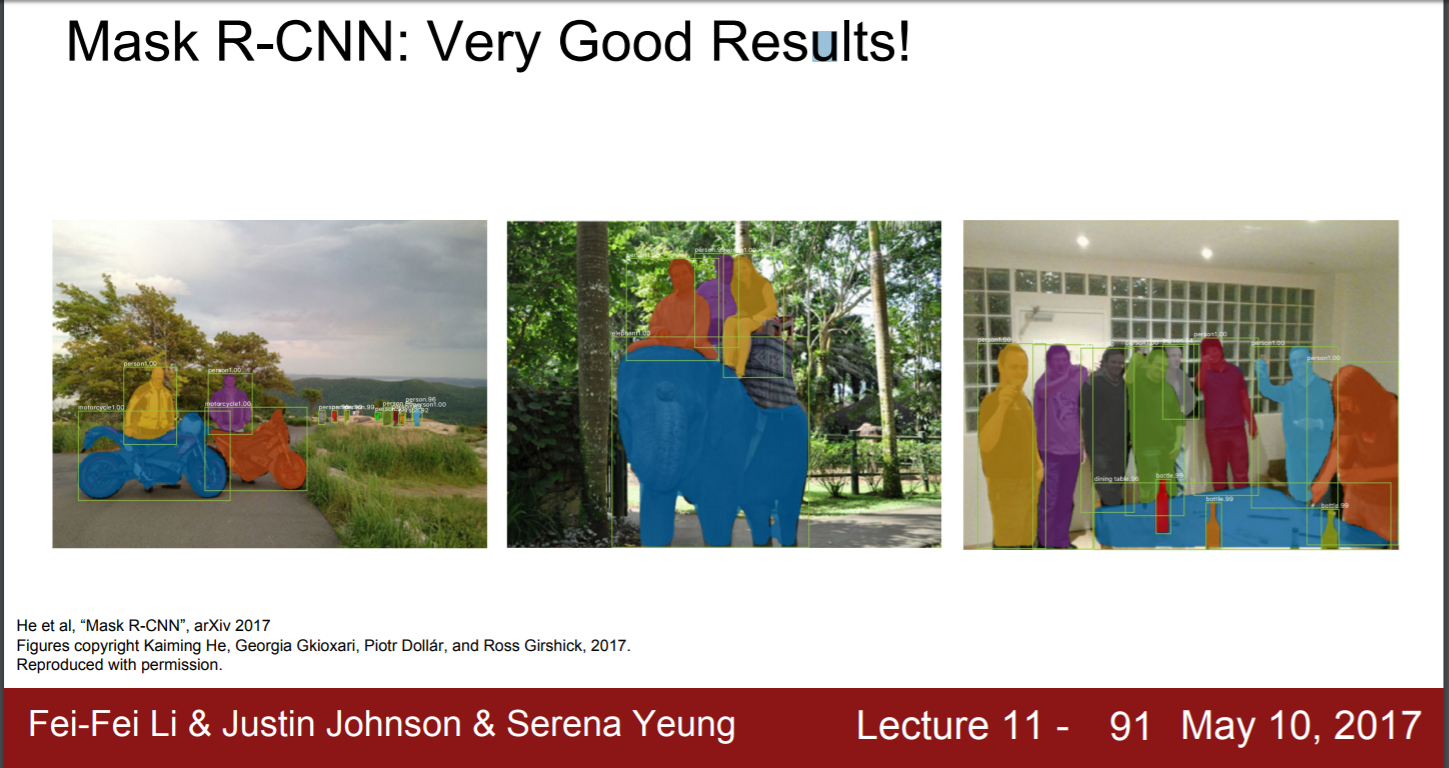
\includegraphics{r-cnn-segment.png}
\caption{}
\end{figure}

    \#

Mask R-CNN Post

\begin{figure}
\centering
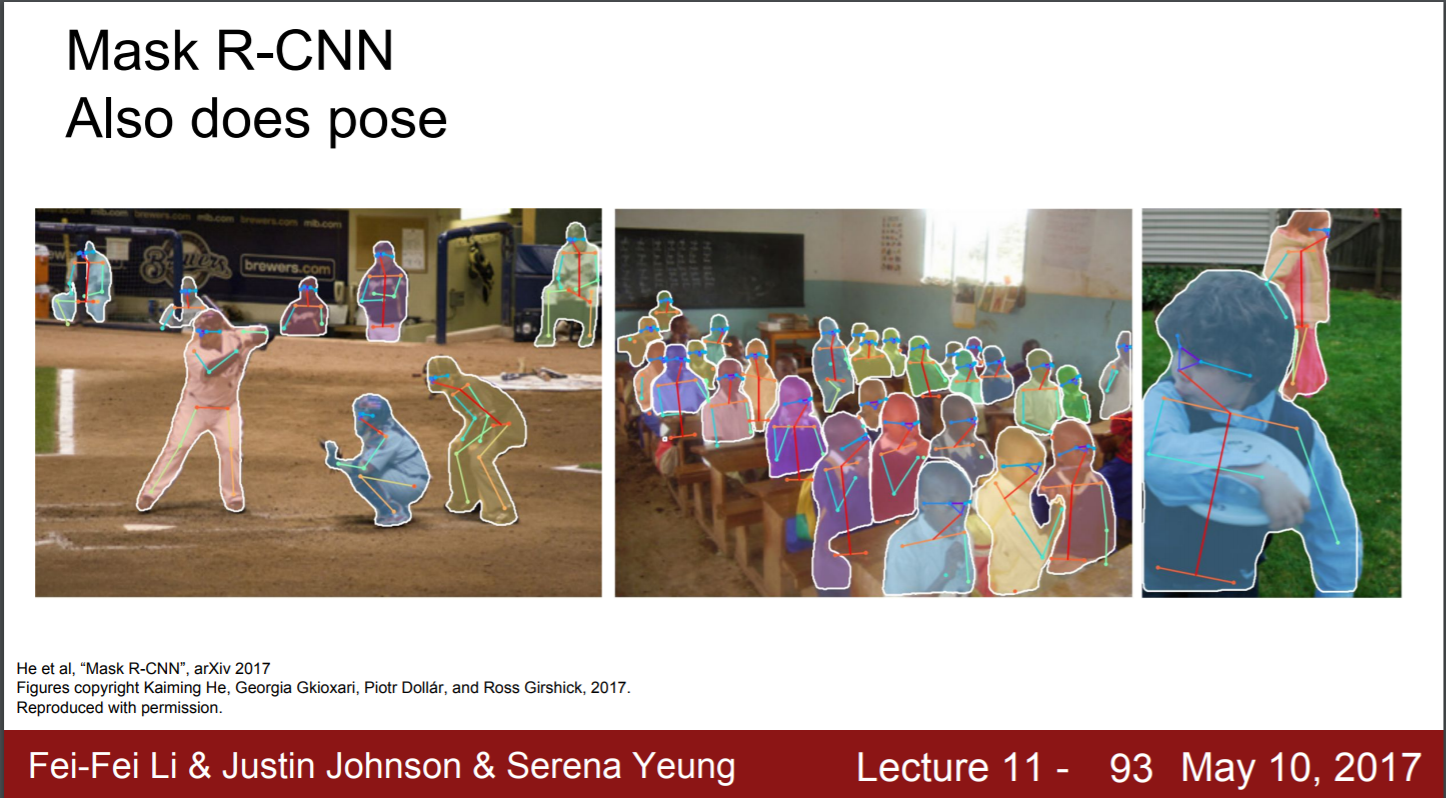
\includegraphics{r-cnn-pose.png}
\caption{}
\end{figure}

    \#

DeepDream

\begin{figure}
\centering
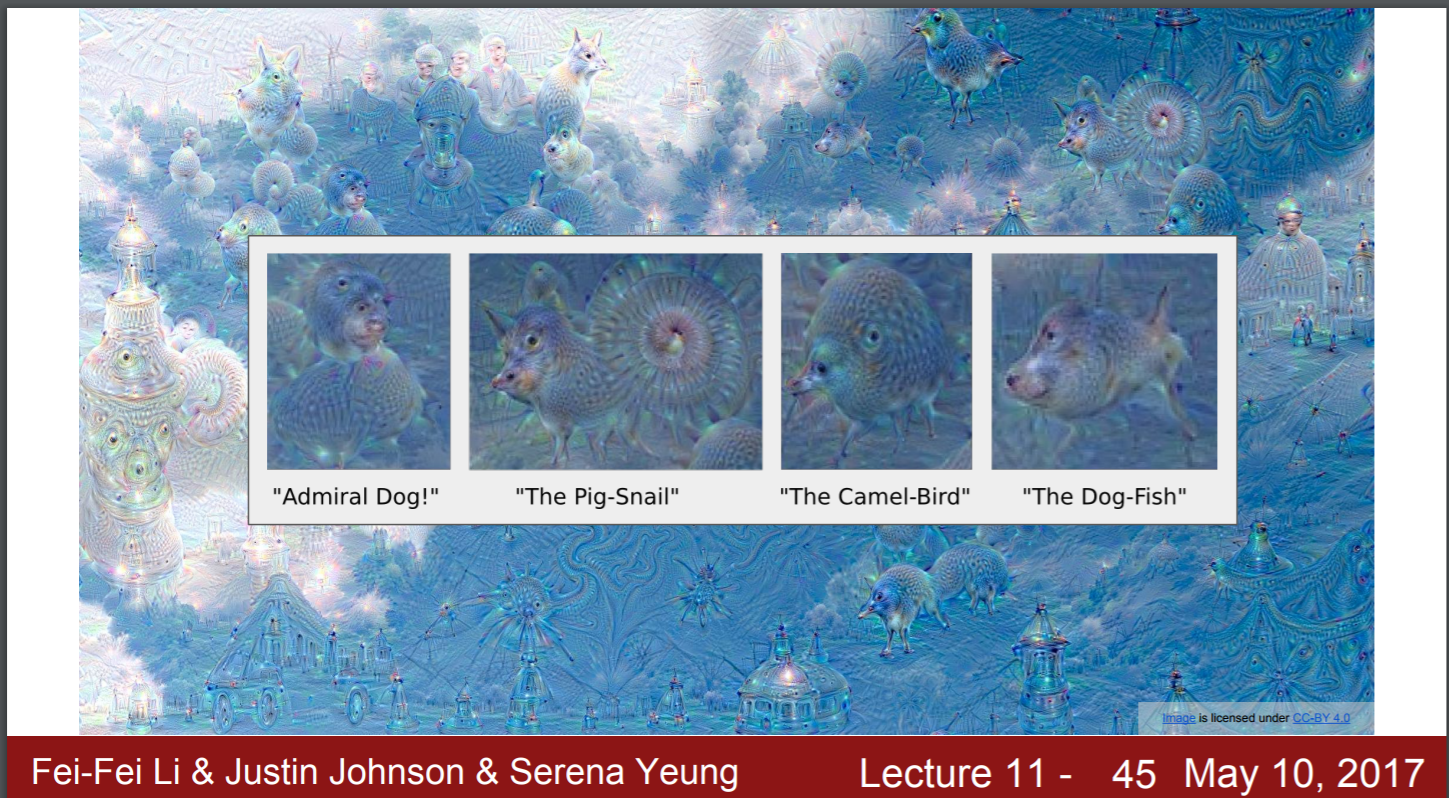
\includegraphics{deepdream.png}
\caption{}
\end{figure}

    \#

Style-transfer

\begin{figure}
\centering
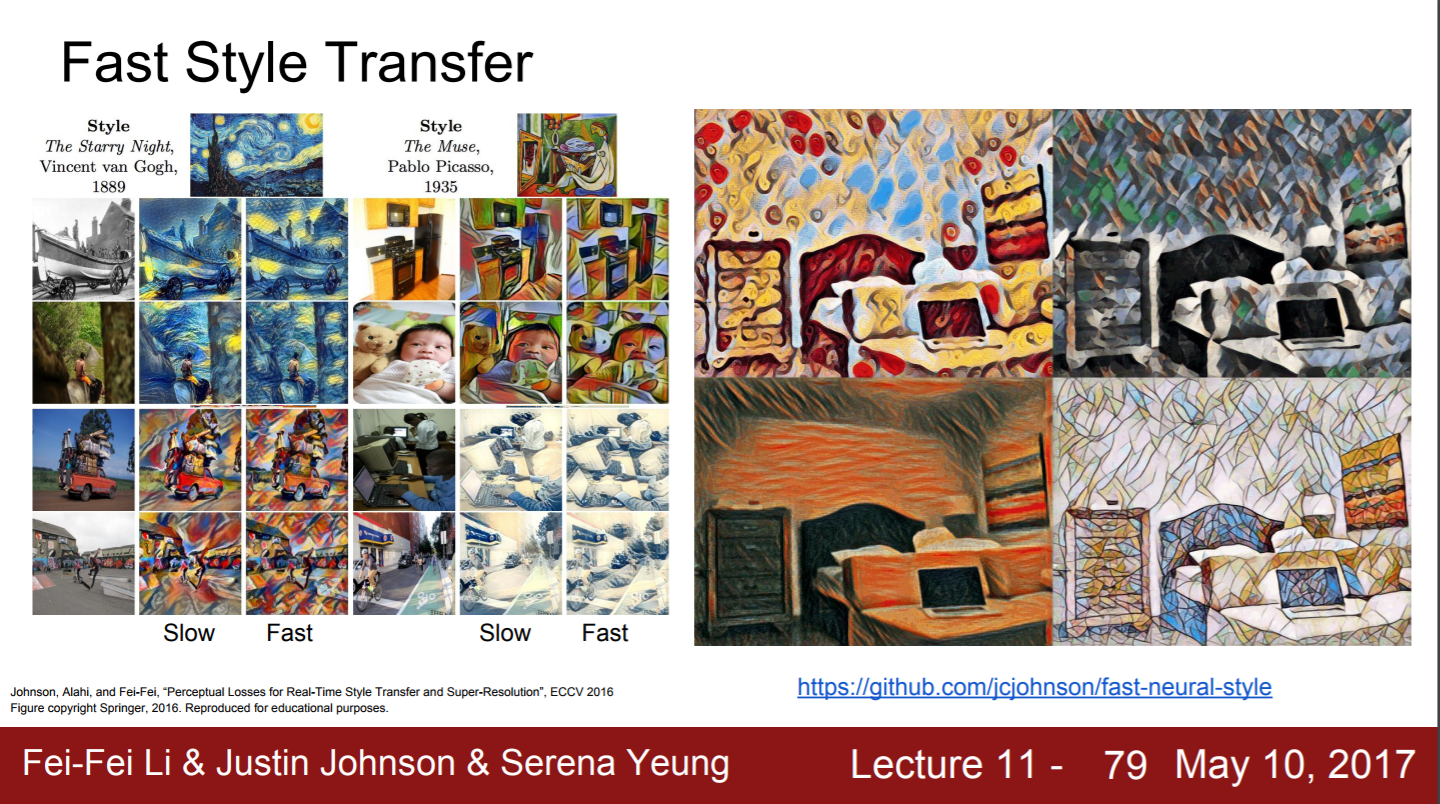
\includegraphics{style-transfer.png}
\caption{}
\end{figure}

    \#

Gramian 矩陣

設 \(A\) 為一個 \(m\times n\) 階實矩陣,\(n\) 階方陣 \(G=[g_{ij}]=A^TA\)
稱為 Gramian 或 Gram 矩陣,也有人稱之為交互乘積 (cross-product)
矩陣。考慮 \(A\) 的行向量表達式
\(A=\begin{bmatrix} \mathbf{a}_1&\mathbf{a}_2&\cdots&\mathbf{a}_n \end{bmatrix}\),\(\mathbf{a}_i\in\mathbb{R}^m\),則:
\[G=A^TA=\begin{bmatrix}  \mathbf{a}_1^T\\    \mathbf{a}_2^T\\    \vdots\\    \mathbf{a}_n^T    \end{bmatrix}\begin{bmatrix}    \mathbf{a}_1&\mathbf{a}_2&\cdots&\mathbf{a}_n    \end{bmatrix}=\begin{bmatrix}    \mathbf{a}_1^T\mathbf{a}_1&\mathbf{a}_1^T\mathbf{a}_2&\cdots&\mathbf{a}_1^T\mathbf{a}_n\\    \mathbf{a}_2^T\mathbf{a}_1&\mathbf{a}_2^T\mathbf{a}_2&\cdots&\mathbf{a}_2^T\mathbf{a}_n\\    ~&~&~&~\\    \mathbf{a}_n^T\mathbf{a}_1&\mathbf{a}_n^T\mathbf{a}_2&\cdots&\mathbf{a}_n^T\mathbf{a}_n    \end{bmatrix}\]

    \begin{Verbatim}[commandchars=\\\{\}]
{\color{incolor}In [{\color{incolor}23}]:} \PY{k+kn}{import} \PY{n+nn}{numpy} \PY{k}{as} \PY{n+nn}{np}
         
         \PY{n}{A} \PY{o}{=} \PY{n}{np}\PY{o}{.}\PY{n}{random}\PY{o}{.}\PY{n}{randint}\PY{p}{(}\PY{l+m+mi}{0}\PY{p}{,}\PY{l+m+mi}{5}\PY{p}{,} \PY{p}{(}\PY{l+m+mi}{2}\PY{p}{,}\PY{l+m+mi}{2}\PY{p}{)}\PY{p}{)}
         
         \PY{n}{B} \PY{o}{=} \PY{n}{np}\PY{o}{.}\PY{n}{dot}\PY{p}{(}\PY{n}{A}\PY{o}{.}\PY{n}{T}\PY{p}{,} \PY{n}{A}\PY{p}{)}
         \PY{n+nb}{print}\PY{p}{(}\PY{n}{A}\PY{p}{)}
         \PY{n+nb}{print}\PY{p}{(}\PY{n}{B}\PY{p}{)}
\end{Verbatim}


    \begin{Verbatim}[commandchars=\\\{\}]
[[1 1]
 [3 4]]
[[10 13]
 [13 17]]

    \end{Verbatim}

    \begin{Verbatim}[commandchars=\\\{\}]
{\color{incolor}In [{\color{incolor}2}]:}         \PY{n}{parser}\PY{o}{.}\PY{n}{add\PYZus{}argument}\PY{p}{(}\PY{l+s+s1}{\PYZsq{}}\PY{l+s+s1}{\PYZhy{}\PYZhy{}content\PYZus{}layers}\PY{l+s+s1}{\PYZsq{}}\PY{p}{,} \PY{n}{nargs}\PY{o}{=}\PY{l+s+s1}{\PYZsq{}}\PY{l+s+s1}{+}\PY{l+s+s1}{\PYZsq{}}\PY{p}{,} \PY{n+nb}{type}\PY{o}{=}\PY{n+nb}{str}\PY{p}{,} \PY{n}{default}\PY{o}{=}\PY{p}{[}\PY{l+s+s1}{\PYZsq{}}\PY{l+s+s1}{conv4\PYZus{}2}\PY{l+s+s1}{\PYZsq{}}\PY{p}{]}\PY{p}{,} \PY{n}{help}\PY{o}{=}\PY{l+s+s1}{\PYZsq{}}\PY{l+s+s1}{VGG19 layers used for content loss}\PY{l+s+s1}{\PYZsq{}}\PY{p}{)}
                \PY{n}{parser}\PY{o}{.}\PY{n}{add\PYZus{}argument}\PY{p}{(}\PY{l+s+s1}{\PYZsq{}}\PY{l+s+s1}{\PYZhy{}\PYZhy{}style\PYZus{}layers}\PY{l+s+s1}{\PYZsq{}}\PY{p}{,} \PY{n}{nargs}\PY{o}{=}\PY{l+s+s1}{\PYZsq{}}\PY{l+s+s1}{+}\PY{l+s+s1}{\PYZsq{}}\PY{p}{,} \PY{n+nb}{type}\PY{o}{=}\PY{n+nb}{str}\PY{p}{,} \PY{n}{default}\PY{o}{=}\PY{p}{[}\PY{l+s+s1}{\PYZsq{}}\PY{l+s+s1}{relu1\PYZus{}1}\PY{l+s+s1}{\PYZsq{}}\PY{p}{,} \PY{l+s+s1}{\PYZsq{}}\PY{l+s+s1}{relu2\PYZus{}1}\PY{l+s+s1}{\PYZsq{}}\PY{p}{,} \PY{l+s+s1}{\PYZsq{}}\PY{l+s+s1}{relu3\PYZus{}1}\PY{l+s+s1}{\PYZsq{}}\PY{p}{,} \PY{l+s+s1}{\PYZsq{}}\PY{l+s+s1}{relu4\PYZus{}1}\PY{l+s+s1}{\PYZsq{}}\PY{p}{,} \PY{l+s+s1}{\PYZsq{}}\PY{l+s+s1}{relu5\PYZus{}1}\PY{l+s+s1}{\PYZsq{}}\PY{p}{]}\PY{p}{,}
                                \PY{n}{help}\PY{o}{=}\PY{l+s+s1}{\PYZsq{}}\PY{l+s+s1}{VGG19 layers used for style loss}\PY{l+s+s1}{\PYZsq{}}\PY{p}{)}
            
                \PY{l+s+sd}{\PYZdq{}\PYZdq{}\PYZdq{}https://github.com/hwalsuklee/tensorflow\PYZhy{}style\PYZhy{}transfer/blob/master/style\PYZus{}transfer.py\PYZdq{}\PYZdq{}\PYZdq{}}
                \PY{l+s+sd}{\PYZdq{}\PYZdq{}\PYZdq{} compute loss \PYZdq{}\PYZdq{}\PYZdq{}}
                \PY{n}{L\PYZus{}content} \PY{o}{=} \PY{l+m+mi}{0}
                \PY{n}{L\PYZus{}style} \PY{o}{=} \PY{l+m+mi}{0}
                \PY{k}{for} \PY{n+nb}{id} \PY{o+ow}{in} \PY{n+nb+bp}{self}\PY{o}{.}\PY{n}{Fs}\PY{p}{:}
                    \PY{k}{if} \PY{n+nb}{id} \PY{o+ow}{in} \PY{n+nb+bp}{self}\PY{o}{.}\PY{n}{CONTENT\PYZus{}LAYERS}\PY{p}{:}
                        \PY{c+c1}{\PYZsh{}\PYZsh{} content loss \PYZsh{}\PYZsh{}}
        
                        \PY{n}{F} \PY{o}{=} \PY{n+nb+bp}{self}\PY{o}{.}\PY{n}{Fs}\PY{p}{[}\PY{n+nb}{id}\PY{p}{]}            \PY{c+c1}{\PYZsh{} content feature of x}
                        \PY{n}{P} \PY{o}{=} \PY{n+nb+bp}{self}\PY{o}{.}\PY{n}{Ps}\PY{p}{[}\PY{n+nb}{id}\PY{p}{]}            \PY{c+c1}{\PYZsh{} content feature of p}
        
                        \PY{n}{\PYZus{}}\PY{p}{,} \PY{n}{h}\PY{p}{,} \PY{n}{w}\PY{p}{,} \PY{n}{d} \PY{o}{=} \PY{n}{F}\PY{o}{.}\PY{n}{get\PYZus{}shape}\PY{p}{(}\PY{p}{)} \PY{c+c1}{\PYZsh{} first return value is batch size (must be one)}
                        \PY{n}{N} \PY{o}{=} \PY{n}{h}\PY{o}{.}\PY{n}{value}\PY{o}{*}\PY{n}{w}\PY{o}{.}\PY{n}{value}        \PY{c+c1}{\PYZsh{} product of width and height}
                        \PY{n}{M} \PY{o}{=} \PY{n}{d}\PY{o}{.}\PY{n}{value}                \PY{c+c1}{\PYZsh{} number of filters}
        
                        \PY{n}{w} \PY{o}{=} \PY{n+nb+bp}{self}\PY{o}{.}\PY{n}{CONTENT\PYZus{}LAYERS}\PY{p}{[}\PY{n+nb}{id}\PY{p}{]}\PY{c+c1}{\PYZsh{} weight for this layer}
        
                        \PY{c+c1}{\PYZsh{} You may choose different normalization constant}
                        \PY{k}{if} \PY{n+nb+bp}{self}\PY{o}{.}\PY{n}{content\PYZus{}loss\PYZus{}norm\PYZus{}type}\PY{o}{==}\PY{l+m+mi}{1}\PY{p}{:}
                            \PY{n}{L\PYZus{}content} \PY{o}{+}\PY{o}{=} \PY{n}{w} \PY{o}{*} \PY{n}{tf}\PY{o}{.}\PY{n}{reduce\PYZus{}sum}\PY{p}{(}\PY{n}{tf}\PY{o}{.}\PY{n}{pow}\PY{p}{(}\PY{p}{(}\PY{n}{F}\PY{o}{\PYZhy{}}\PY{n}{P}\PY{p}{)}\PY{p}{,} \PY{l+m+mi}{2}\PY{p}{)}\PY{p}{)} \PY{o}{/} \PY{l+m+mi}{2} \PY{c+c1}{\PYZsh{} original paper}
                        \PY{k}{elif} \PY{n+nb+bp}{self}\PY{o}{.}\PY{n}{content\PYZus{}loss\PYZus{}norm\PYZus{}type} \PY{o}{==} \PY{l+m+mi}{2}\PY{p}{:}
                            \PY{n}{L\PYZus{}content} \PY{o}{+}\PY{o}{=} \PY{n}{w} \PY{o}{*} \PY{n}{tf}\PY{o}{.}\PY{n}{reduce\PYZus{}sum}\PY{p}{(}\PY{n}{tf}\PY{o}{.}\PY{n}{pow}\PY{p}{(}\PY{p}{(}\PY{n}{F}\PY{o}{\PYZhy{}}\PY{n}{P}\PY{p}{)}\PY{p}{,} \PY{l+m+mi}{2}\PY{p}{)}\PY{p}{)} \PY{o}{/} \PY{p}{(}\PY{n}{N}\PY{o}{*}\PY{n}{M}\PY{p}{)} \PY{c+c1}{\PYZsh{}artistic style transfer for videos}
                        \PY{k}{elif} \PY{n+nb+bp}{self}\PY{o}{.}\PY{n}{content\PYZus{}loss\PYZus{}norm\PYZus{}type} \PY{o}{==} \PY{l+m+mi}{3}\PY{p}{:} \PY{c+c1}{\PYZsh{} this is from https://github.com/cysmith/neural\PYZhy{}style\PYZhy{}tf/blob/master/neural\PYZus{}style.py}
                            \PY{n}{L\PYZus{}content} \PY{o}{+}\PY{o}{=} \PY{n}{w} \PY{o}{*} \PY{p}{(}\PY{l+m+mf}{1.} \PY{o}{/} \PY{p}{(}\PY{l+m+mf}{2.} \PY{o}{*} \PY{n}{np}\PY{o}{.}\PY{n}{sqrt}\PY{p}{(}\PY{n}{M}\PY{p}{)} \PY{o}{*} \PY{n}{np}\PY{o}{.}\PY{n}{sqrt}\PY{p}{(}\PY{n}{N}\PY{p}{)}\PY{p}{)}\PY{p}{)} \PY{o}{*} \PY{n}{tf}\PY{o}{.}\PY{n}{reduce\PYZus{}sum}\PY{p}{(}\PY{n}{tf}\PY{o}{.}\PY{n}{pow}\PY{p}{(}\PY{p}{(}\PY{n}{F} \PY{o}{\PYZhy{}} \PY{n}{P}\PY{p}{)}\PY{p}{,} \PY{l+m+mi}{2}\PY{p}{)}\PY{p}{)}
        
                    \PY{k}{elif} \PY{n+nb}{id} \PY{o+ow}{in} \PY{n+nb+bp}{self}\PY{o}{.}\PY{n}{STYLE\PYZus{}LAYERS}\PY{p}{:}
                        \PY{c+c1}{\PYZsh{}\PYZsh{} style loss \PYZsh{}\PYZsh{}}
        
                        \PY{n}{F} \PY{o}{=} \PY{n+nb+bp}{self}\PY{o}{.}\PY{n}{Fs}\PY{p}{[}\PY{n+nb}{id}\PY{p}{]}
        
                        \PY{n}{\PYZus{}}\PY{p}{,} \PY{n}{h}\PY{p}{,} \PY{n}{w}\PY{p}{,} \PY{n}{d} \PY{o}{=} \PY{n}{F}\PY{o}{.}\PY{n}{get\PYZus{}shape}\PY{p}{(}\PY{p}{)}  \PY{c+c1}{\PYZsh{} first return value is batch size (must be one)}
                        \PY{n}{N} \PY{o}{=} \PY{n}{h}\PY{o}{.}\PY{n}{value} \PY{o}{*} \PY{n}{w}\PY{o}{.}\PY{n}{value}       \PY{c+c1}{\PYZsh{} product of width and height}
                        \PY{n}{M} \PY{o}{=} \PY{n}{d}\PY{o}{.}\PY{n}{value}                 \PY{c+c1}{\PYZsh{} number of filters}
        
                        \PY{n}{w} \PY{o}{=} \PY{n+nb+bp}{self}\PY{o}{.}\PY{n}{STYLE\PYZus{}LAYERS}\PY{p}{[}\PY{n+nb}{id}\PY{p}{]}   \PY{c+c1}{\PYZsh{} weight for this layer}
        
                        \PY{n}{G} \PY{o}{=} \PY{n+nb+bp}{self}\PY{o}{.}\PY{n}{\PYZus{}gram\PYZus{}matrix}\PY{p}{(}\PY{n}{F}\PY{p}{)}    \PY{c+c1}{\PYZsh{} style feature of x}
                        \PY{n}{A} \PY{o}{=} \PY{n+nb+bp}{self}\PY{o}{.}\PY{n}{As}\PY{p}{[}\PY{n+nb}{id}\PY{p}{]}             \PY{c+c1}{\PYZsh{} style feature of a}
        
                        \PY{n}{L\PYZus{}style} \PY{o}{+}\PY{o}{=} \PY{n}{w} \PY{o}{*} \PY{p}{(}\PY{l+m+mf}{1.} \PY{o}{/} \PY{p}{(}\PY{l+m+mi}{4} \PY{o}{*} \PY{n}{N} \PY{o}{*}\PY{o}{*} \PY{l+m+mi}{2} \PY{o}{*} \PY{n}{M} \PY{o}{*}\PY{o}{*} \PY{l+m+mi}{2}\PY{p}{)}\PY{p}{)} \PY{o}{*} \PY{n}{tf}\PY{o}{.}\PY{n}{reduce\PYZus{}sum}\PY{p}{(}\PY{n}{tf}\PY{o}{.}\PY{n}{pow}\PY{p}{(}\PY{p}{(}\PY{n}{G}\PY{o}{\PYZhy{}}\PY{n}{A}\PY{p}{)}\PY{p}{,} \PY{l+m+mi}{2}\PY{p}{)}\PY{p}{)}
\end{Verbatim}


    \begin{Verbatim}[commandchars=\\\{\}]

          File "<ipython-input-2-e8223f7ccc10>", line 2
        L\_content = 0
        \^{}
    IndentationError: unexpected indent
    

    \end{Verbatim}

    \#

CNN GAN

\begin{figure}
\centering
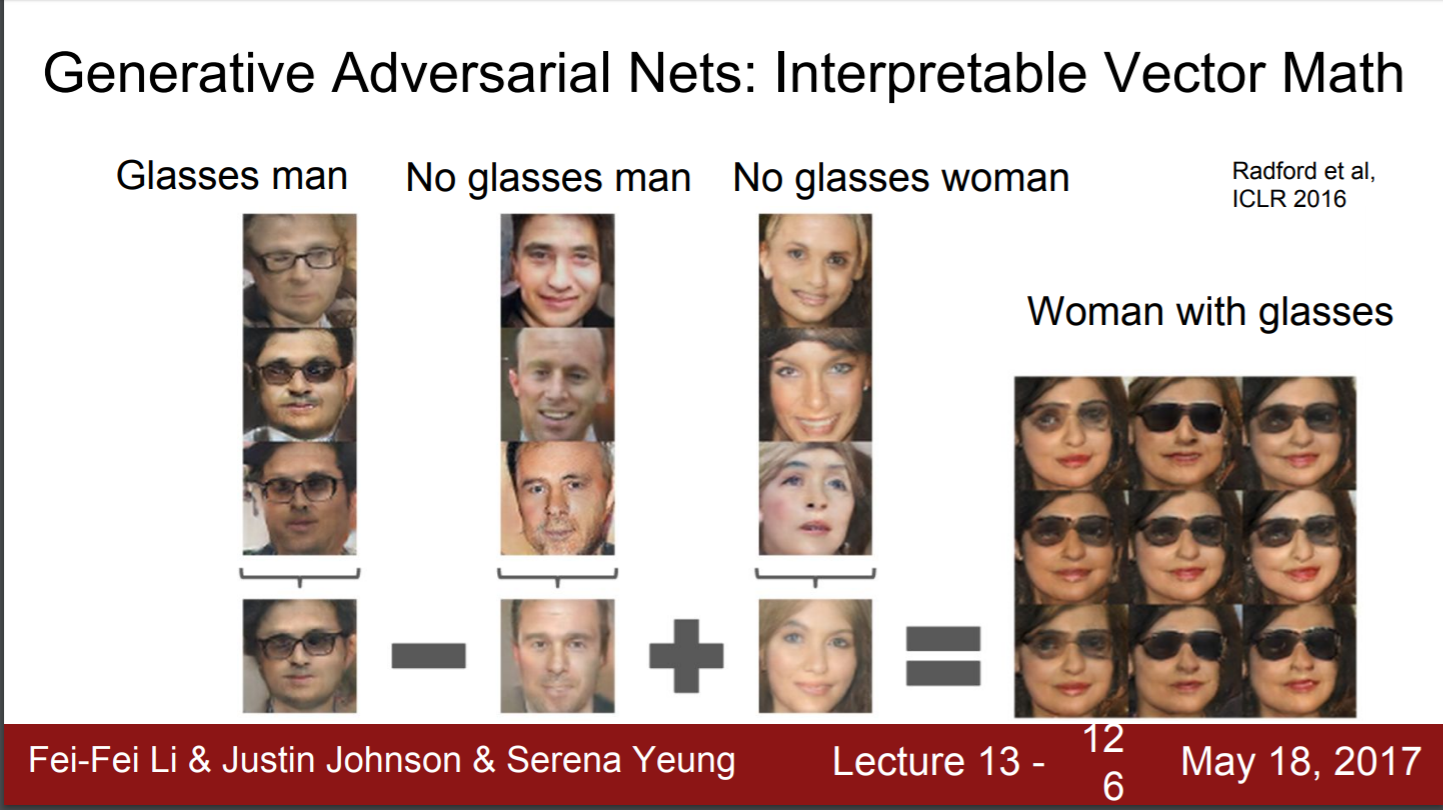
\includegraphics{gan.png}
\caption{}
\end{figure}

    \#

GAN Training

\begin{figure}
\centering
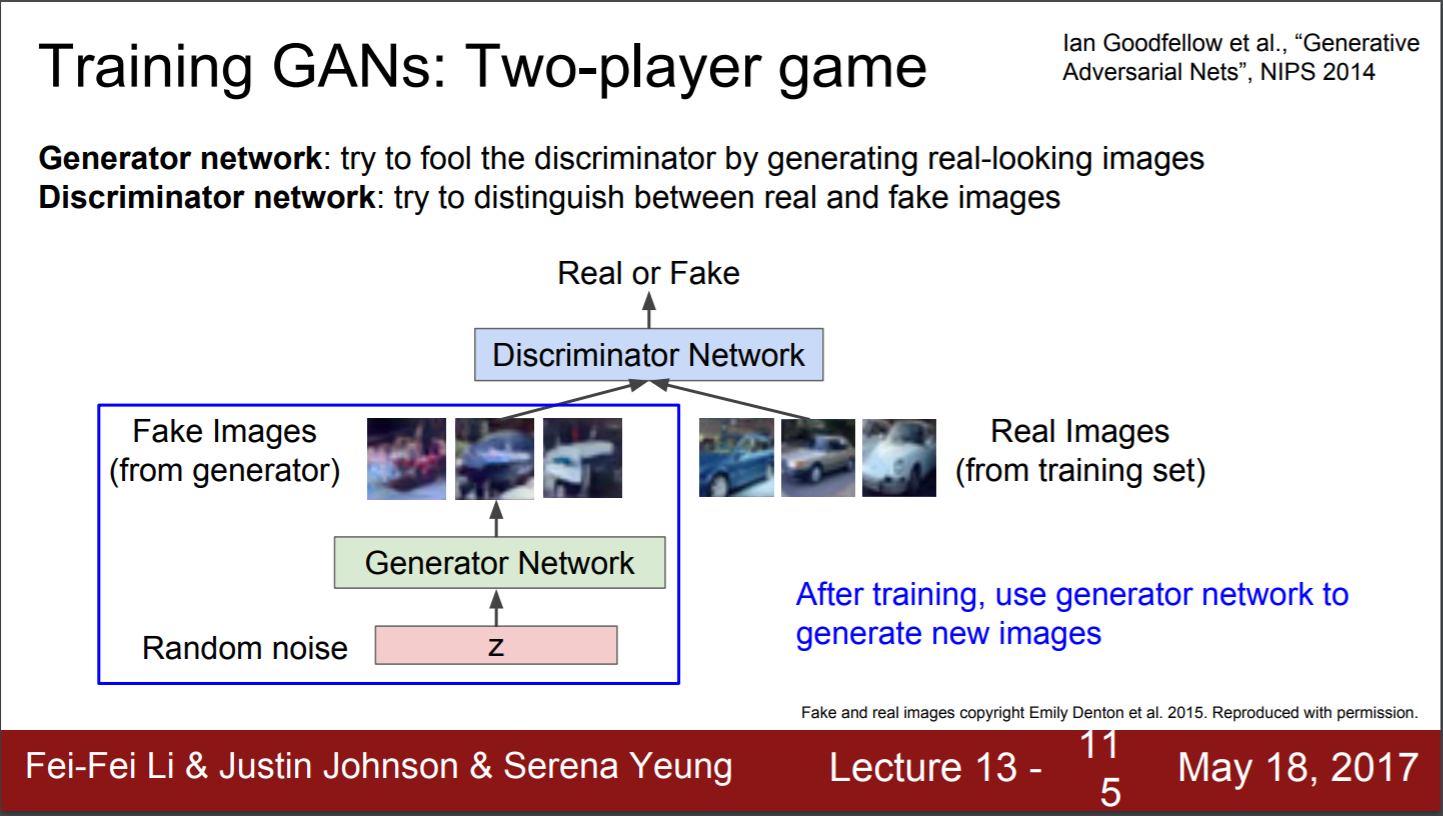
\includegraphics{gan-training.png}
\caption{}
\end{figure}

    \#

Sequential Model

\begin{figure}
\centering
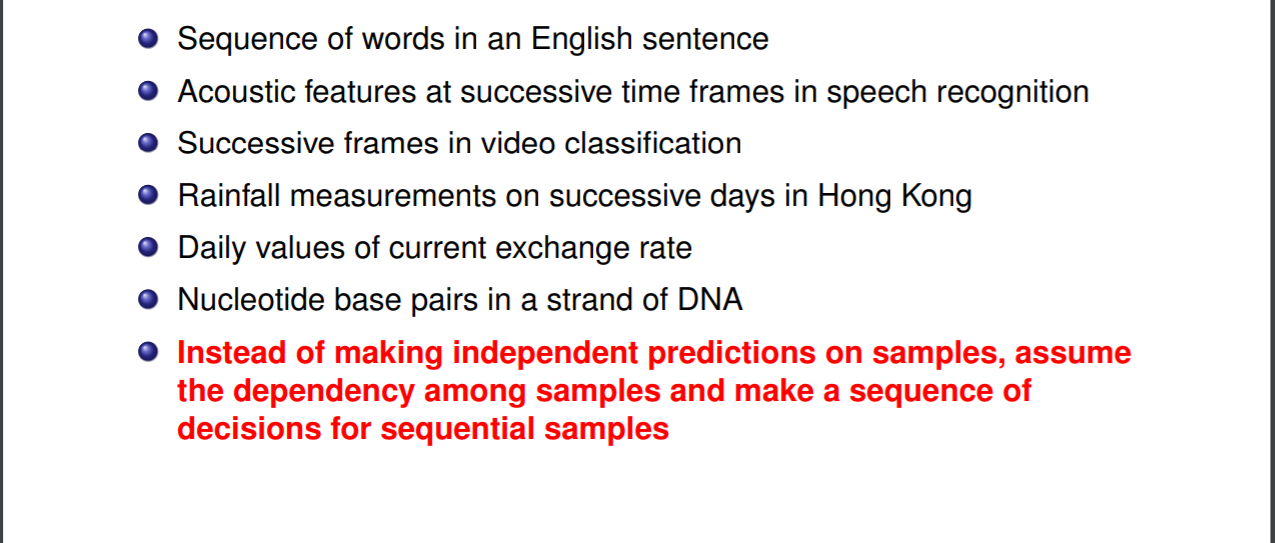
\includegraphics{sequence.png}
\caption{}
\end{figure}

    \begin{figure}
\centering
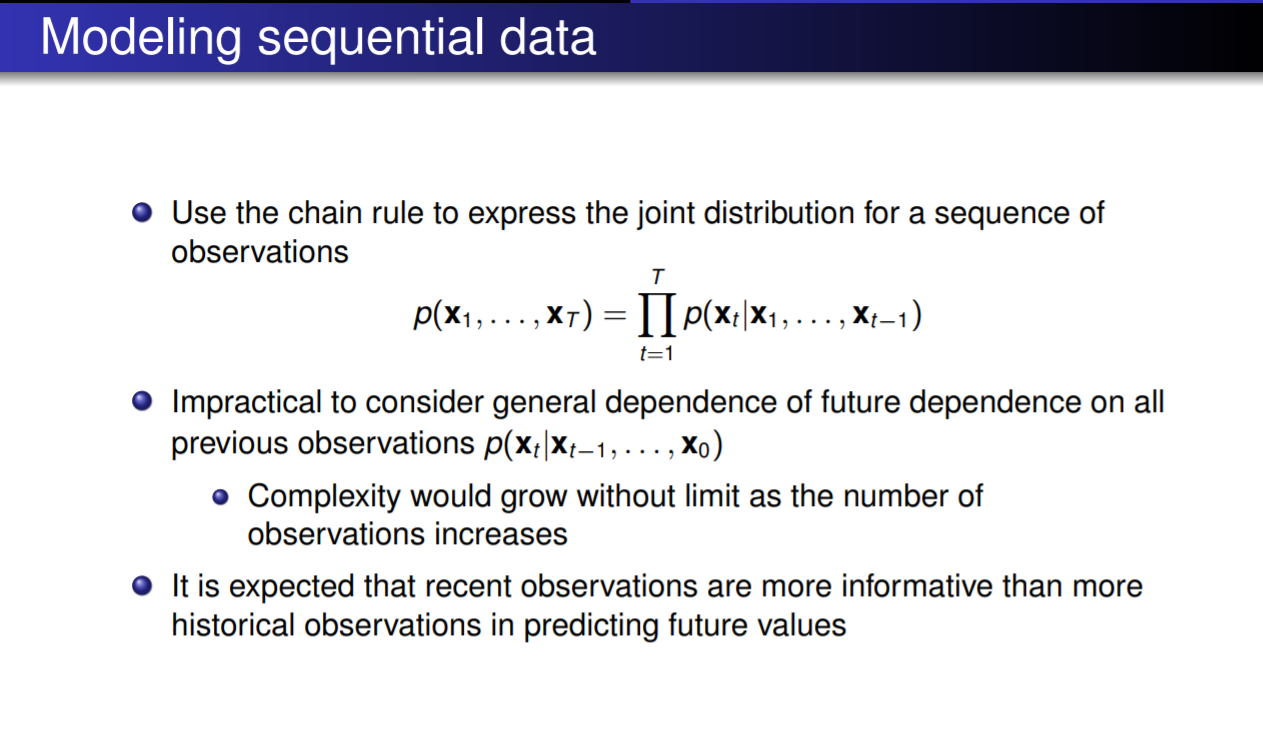
\includegraphics{model_sequence.png}
\caption{}
\end{figure}

    \#

Markov model

\begin{figure}
\centering
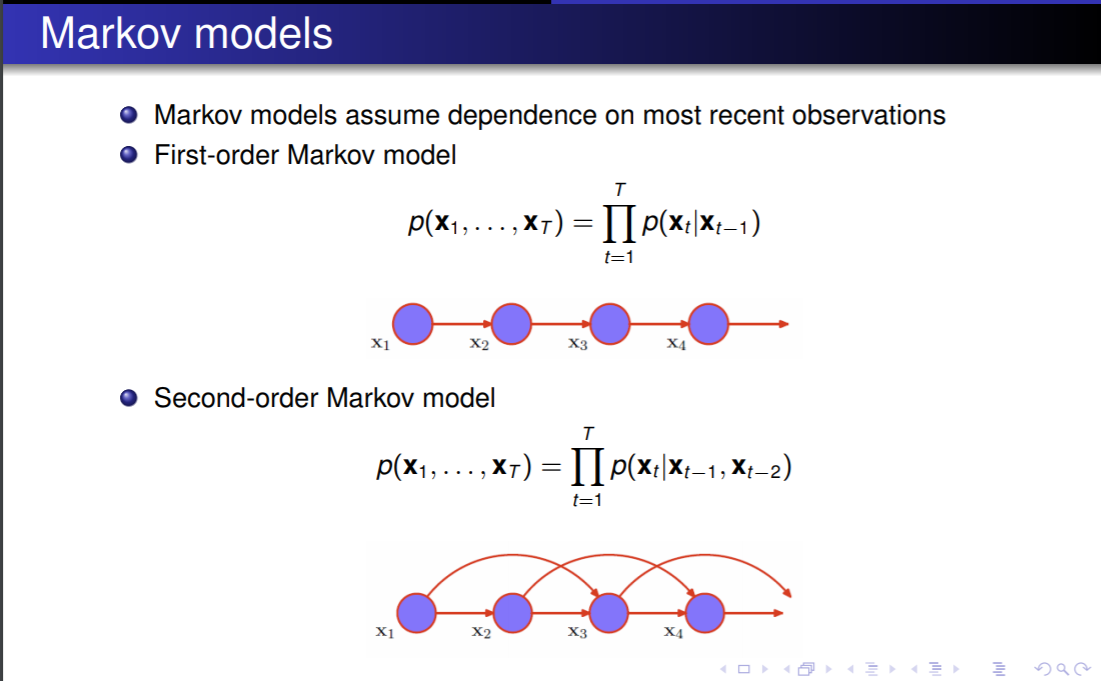
\includegraphics{markov.png}
\caption{}
\end{figure}

    \#

Markov model

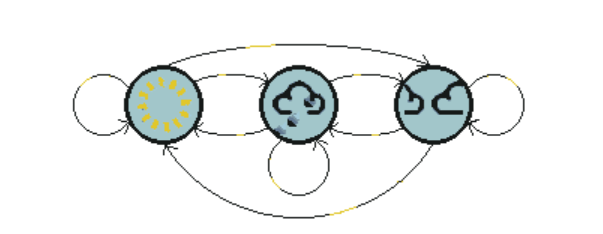
\includegraphics{weather.png} \#

Hidden Markov model

\begin{figure}
\centering
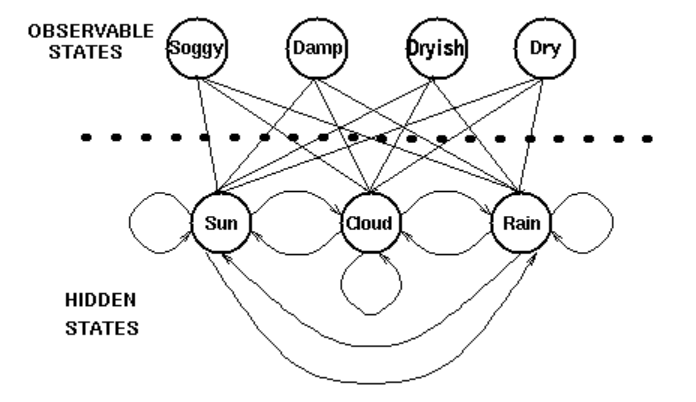
\includegraphics{weather1.png}
\caption{}
\end{figure}

    \#

Hidden Markov model

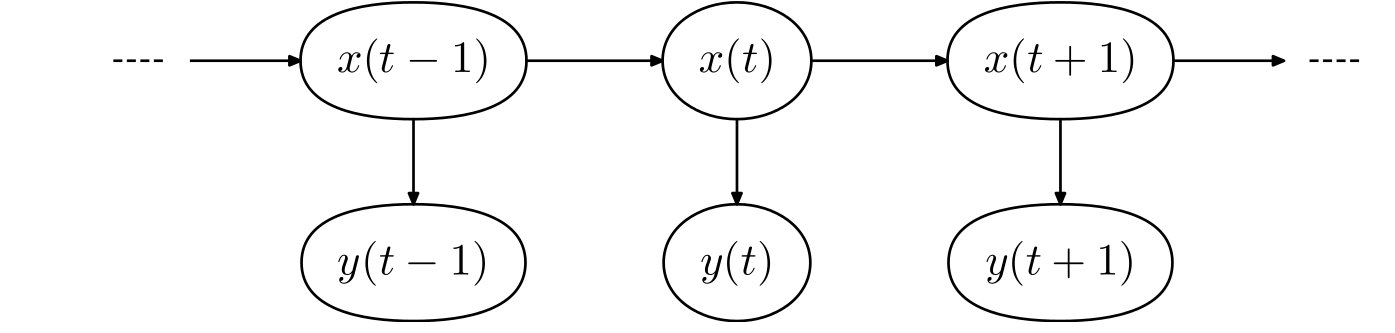
\includegraphics{HMM.png} \#

HMM 输入法应用

\begin{figure}
\centering
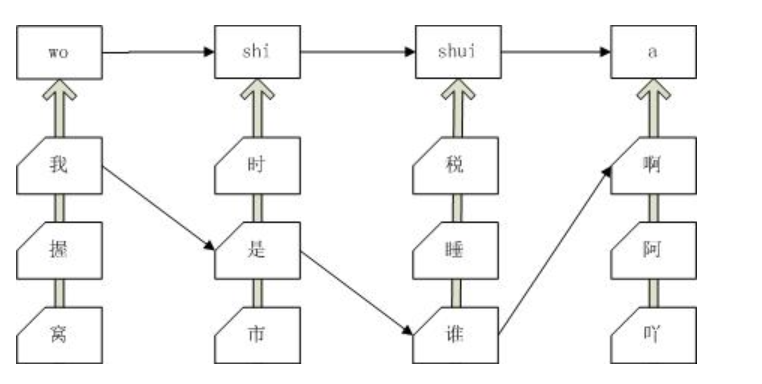
\includegraphics{输入法.png}
\caption{}
\end{figure}

    \#

RNN

\begin{center}\rule{0.5\linewidth}{\linethickness}\end{center}

\begin{itemize}
\tightlist
\item
  image captioning
\item
  sentiment classification
\item
  machine translation
\item
  video classification on frame level
\end{itemize}

\begin{figure}
\centering
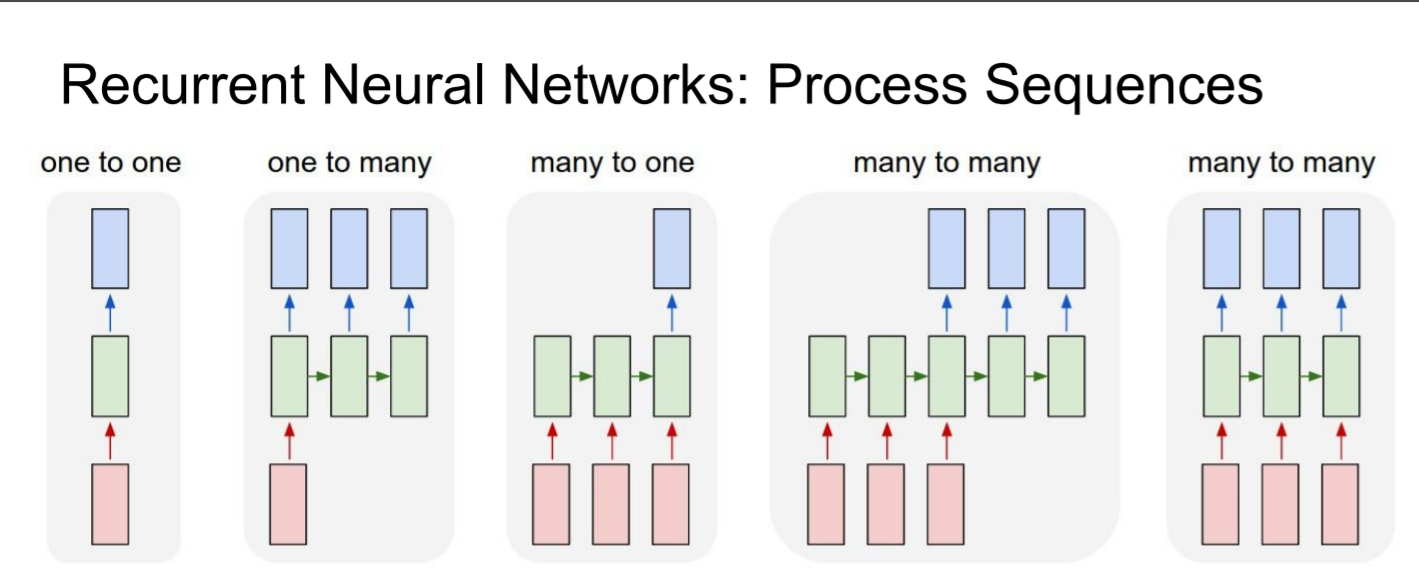
\includegraphics{rnn-model.png}
\caption{}
\end{figure}

    \#

RNN

\subsection{\texorpdfstring{\({h_t} = \tan ({W_{{\rm{x}}h}}{x_{_t}} + {W_{hh}}{h_{t - 1}} + b)\)}{\{h\_t\} = \textbackslash{}tan (\{W\_\{\{\textbackslash{}rm\{x\}\}h\}\}\{x\_\{\_t\}\} + \{W\_\{hh\}\}\{h\_\{t - 1\}\} + b)}}\label{h_t-tan-w_rmxhx__t-w_hhh_t---1-b}

\begin{figure}
\centering
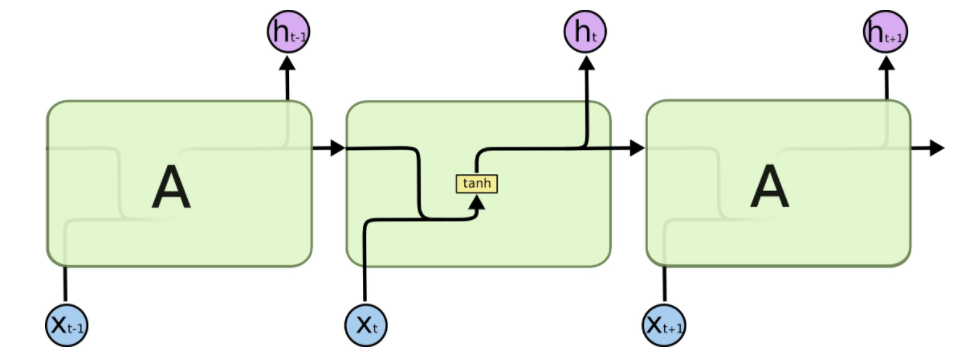
\includegraphics{rnn.png}
\caption{}
\end{figure}

    \#

LSTM

Colah LSTM:http://colah.github.io/posts/2015-08-Understanding-LSTMs/

Colah中文版: https://www.yunaitong.cn/understanding-lstm-networks.html
\includegraphics{lstm.png}

    \#

Image Captioning

\begin{figure}
\centering
\includegraphics{rnn_straw.png}
\caption{}
\end{figure}

    \begin{figure}
\centering
\includegraphics{image_caption.png}
\caption{}
\end{figure}

    \begin{figure}
\centering
\includegraphics{rnn-code.png}
\caption{}
\end{figure}

    \begin{figure}
\centering
\includegraphics{rnn-answer.png}
\caption{}
\end{figure}

    \begin{figure}
\centering
\includegraphics{rnn-hard.png}
\caption{}
\end{figure}

    \#

Reinforcement Learning

\begin{center}\rule{0.5\linewidth}{\linethickness}\end{center}

\begin{figure}
\centering
\includegraphics{reinforcement.png}
\caption{}
\end{figure}

    \begin{figure}
\centering
\includegraphics{alphago.png}
\caption{}
\end{figure}

    \#

Q-learning

Q-learning demo
英文版:http://mnemstudio.org/path-finding-q-learning-tutorial.htm

Q-learning demo 中文版: http://www.cnblogs.com/stevenbush/p/3359603.html

\begin{figure}
\centering
\includegraphics{Q-learning.png}
\caption{}
\end{figure}

    \begin{figure}
\centering
\includegraphics{door.png}
\caption{}
\end{figure}

    \begin{figure}
\centering
\includegraphics{door-state.png}
\caption{}
\end{figure}

    \begin{figure}
\centering
\includegraphics{R.png}
\caption{}
\end{figure}

\(\begin{array}{l} Q\left( {1,5} \right) = R\left( {1,5} \right) + 0.8 * \max \{ Q(5,1),Q(5,4),Q(5,5)\} = 100 + 0.8*\max \{ 0,0,0\} = 100 \end{array}\)
\includegraphics{Q.png}

    \includegraphics{Q-end.png} \includegraphics{q-result.png}

    \begin{figure}
\centering
\includegraphics{Q-para.png}
\caption{}
\end{figure}

    \begin{Verbatim}[commandchars=\\\{\}]
{\color{incolor}In [{\color{incolor}2}]:} \PY{k+kn}{from} \PY{n+nn}{IPython}\PY{n+nn}{.}\PY{n+nn}{display} \PY{k}{import} \PY{n}{HTML}
        
        \PY{c+c1}{\PYZsh{} Youtube}
        \PY{n}{HTML}\PY{p}{(}\PY{l+s+s1}{\PYZsq{}}\PY{l+s+s1}{\PYZlt{}iframe width=}\PY{l+s+s1}{\PYZdq{}}\PY{l+s+s1}{720}\PY{l+s+s1}{\PYZdq{}}\PY{l+s+s1}{ height=}\PY{l+s+s1}{\PYZdq{}}\PY{l+s+s1}{480}\PY{l+s+s1}{\PYZdq{}}\PY{l+s+s1}{ src=}\PY{l+s+s1}{\PYZdq{}}\PY{l+s+s1}{Bidirectionally\PYZhy{}Coordinated Nets (BiCNet) for Playing StarCraft Combats.mp4?rel=0\PYZam{}amp;controls=0\PYZam{}amp;showinfo=0}\PY{l+s+s1}{\PYZdq{}}\PY{l+s+s1}{ frameborder=}\PY{l+s+s1}{\PYZdq{}}\PY{l+s+s1}{0}\PY{l+s+s1}{\PYZdq{}}\PY{l+s+s1}{ allowfullscreen\PYZgt{}\PYZlt{}/iframe\PYZgt{}}\PY{l+s+s1}{\PYZsq{}}\PY{p}{)}
\end{Verbatim}


\begin{Verbatim}[commandchars=\\\{\}]
{\color{outcolor}Out[{\color{outcolor}2}]:} <IPython.core.display.HTML object>
\end{Verbatim}
            
    \#

Mastering StarCraft with AI

Researchers from Alibaba and University College London developed a deep
learning-based system that learned how to execute a number of strategies
for the popular real-time strategy game StarCraft.

\begin{figure}
\centering
\includegraphics{STARCRAFT.png}
\caption{}
\end{figure}

    \#

ML问题点

\begin{itemize}
\tightlist
\item
  size
\item
  time
\item
  energy
\end{itemize}

    \begin{figure}
\centering
\includegraphics{ml_problem1.png}
\caption{}
\end{figure}

    \begin{figure}
\centering
\includegraphics{ml_problem2.png}
\caption{}
\end{figure}

    \begin{figure}
\centering
\includegraphics{ml_problem3.png}
\caption{}
\end{figure}


    % Add a bibliography block to the postdoc
    
    
    
    \end{document}
